\documentclass[../main.tex]{subfiles}
\graphicspath{{\subfix{..}}}

\begin{document}
\chapter{The JUNO experiment}
\label{sec:juno}

\epigraph{``Ave Juno, rosae rosam, et spiritus rex''. It means nothing but I found it in tone.}

\minitoc

The first idea of a medium baseline ($\sim$52 km) experiment, was explored in 2008 \cite{zhan_determination_2008} where it was demonstrated that the Neutrino Mass Ordering (NMO) could be determined by a medium baseline experiment if $\sin^2(2\theta_{13}) > 0.005$ without the requirements of accurate knowledge of the reactor antineutrino spectra and the value of $\Delta m_{32}^2$. From this idea is born the Jiangmen Underground Neutrino Observatory (JUNO) experiment.

JUNO is a neutrino detection experiment under construction located in China, in Guangdong proving, near the city of Kaiping. Its main objectives are the determination of the mass ordering at the 3-4$\sigma$ level in 6 years of data taking and the measurement at the sub-percent precision of the oscillation parameters $\Delta m_{21}^2$, $\sin^2 \theta_{12}$, $\Delta m_{32}^2$ and with less precision $\sin^2\theta_{13}$\cite{an_neutrino_2016}.

\begin{figure}[ht]
  \centering
  \begin{subfigure}[b]{0.48\textwidth}
    \centering
    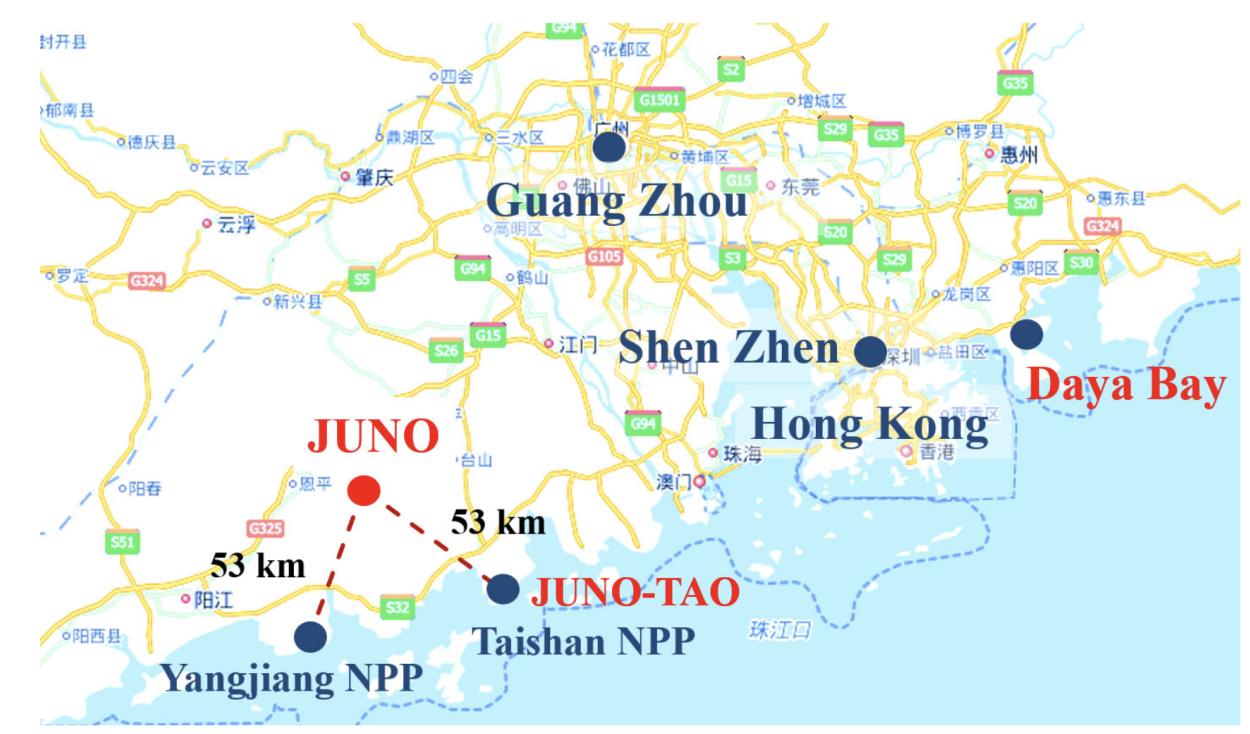
\includegraphics[width=\textwidth]{images/juno/juno_location.png}
  \end{subfigure}
  \hfill
  \begin{subfigure}[b]{0.48\textwidth}
    \centering
    \includegraphics[width=\textwidth]{images/juno/juno_outside.jpg}
  \end{subfigure}
  \caption{\textbf{On the left:} Location of the JUNO experiment and its reactor sources in southern china. \textbf{On the right:} Aerial view of the experimental site}
\end{figure}

For this JUNO will measure the electronic anti-neutrinos ($\bar{\nu}_e$) flux coming from the nuclear reactors of Taishan, Yangjiang, for a total power of 26.6 GW$_{th}$, and the Daya Bay power plant to a lesser extent. All of those cores are the second-generation pressurized water reactors CPR1000, which is a derivative of Framatome M310. Details about the power plants characteristics and their expected flux of $\bar{\nu}_e$ can be found in the table \ref{tab:juno:power_plants}.
The distance of 53 km has been specifically chosen to maximize the disappearance probability of the $\bar{\nu}_e$. The data taking is scheduled to start early 2025.

\section{Reactor Neutrinos physics in JUNO}

JUNO will try to determine the NMO and to bring at the few per mille level our knowledge of $\Delta m^2_{31}$,  $\Delta m^2_{21}$ and $\sin^2(2\theta_{12})$  via the precision analysis of the spectrum of the visible energy left by reactor antineutrinos in its detector.

\begin{figure}
  \centering
  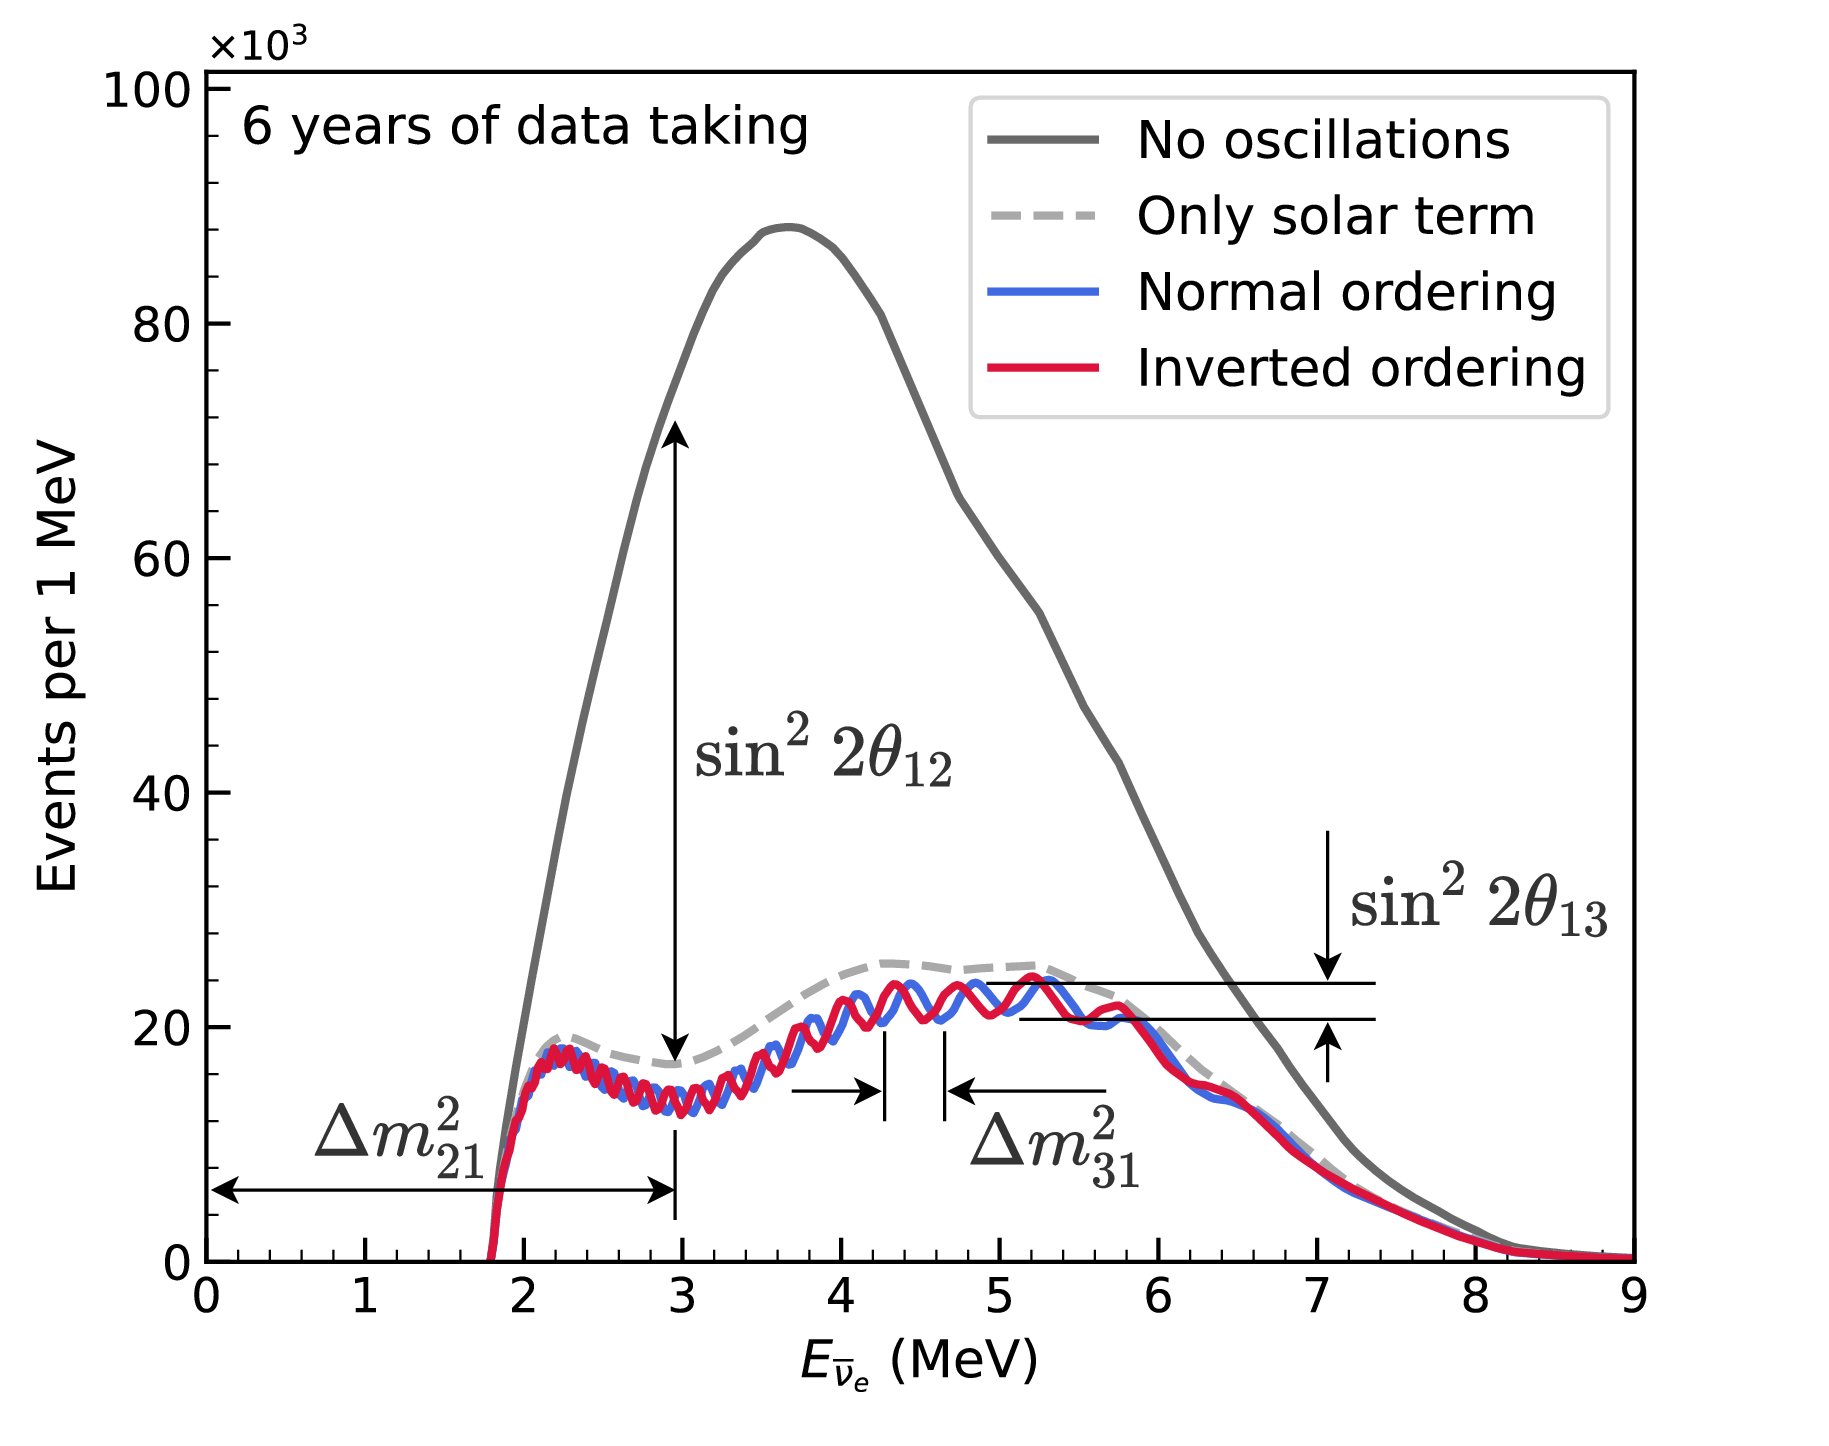
\includegraphics[height=8cm]{images/juno/Spectrum-OscillationsOnly_dm2_31.png}
  \caption{Expected number of neutrinos event per MeV in JUNO after 6 years of data taking. The black curve shows the flux if there was no oscillation. The light gray curve shows the oscillation if only the solar terms are taken in account ($\theta_{12}$, $\Delta m_{21}^2$). The blue and red curve shows the spectrum in the case of, respectively, NO and IO. The dependency of the oscillation to the different parameters are schematized by the double sided arrows. We can see the NMO sensitivity by looking at the fine phase shift between the red and the blue curve.}
  \label{fig:juno:juno-spectrum-oscillation}
\end{figure}

\subsection{Antineutrino spectrum measured in JUNO}
\label{sec:juno:nom_precise_measurement}
To some extent, this analysis is equivalent to to extracting from this spectrum the oscillation probability \cite{an_neutrino_2016} :
\begin{equation*}
  \label{eq:juno:oscillation_prob}
  P(\bnue \rightarrow \bnue) = 1 - \sin^2 2\theta_{12} c^4_{13} \sin^2 \frac{\Delta m^2_{21}L}{4E} - \sin^2 2\theta_{13} \bigg[ c_{12}^2 \sin^2 \frac{\Delta m_{31}^2 L}{4E} + s^2_{12} \sin^2 \frac{\Delta m_{32}^2 L}{4E} \bigg]
\end{equation*}
Where $s_{ij} = \sin \theta_{ij}$, $c_{ij} = \cos \theta_{ij}$, $E$ is the $\bnue$ energy and $L$ is the baseline.
We can see the sensitivity to the NMO in the dependency to $\Delta m_{32}^2$ and $\Delta m^2_{31}$ causing a phase shift of the spectrum as we can see in the Figure \ref{fig:juno:juno-spectrum-oscillation}.

In practice, a fit to the grey distribution of Figure \ref{fig:juno:spectrum_with_background} will be performed. It is the sum of two components :signal (black) and bacgrounds (colored). Reactor antineutrinos are detected by JUNO via Inverse Beta Decays (IBD) : $\bar{nu}_e + p -> e^{+} + n$.
The energy spectrum under investigation is therefore that of the reconstructed $e^+$ visible energy. The black signal spectrum is therefore the sum of the antineutrino differential fluxes from all reactors and reaching the detecteur, weighted by the oscillation probability of Eq \ref{eq:juno:oscillation_prob} and the IBD differential cross section and convoluted with detection effects.
These various ingredients are theoretically modelled in order to provide the probability density function (PDF) to be used in the fit.

\begin{figure}[ht]
  \centering
  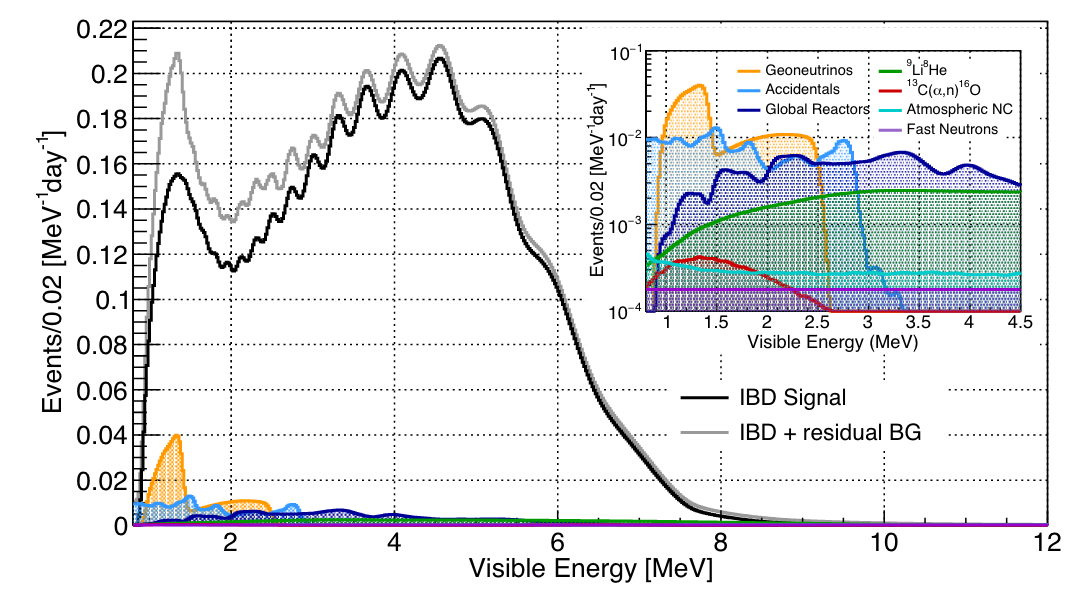
\includegraphics[height=6cm]{images/juno/spectrum_with_background.png}
  \caption{Expected visible energy spectrum measured with the LPMT system with (grey) and without (black) backgrounds. The background amount for about 7\% of the IBD candidate and are mostly localized below 3 MeV \cite{juno_collaboration_sub-percent_2022}}
  \label{fig:juno:spectrum_with_background}
\end{figure}

To reach JUNO's goals, it takes that this experimental spectrum still bears sizeable traces of the very small phase shift mentioned above. Most notably, the
following requirements must be fulfilled :
\begin{enumerate}
  \item An energy resolution of $3\%/\sqrt{E\mathrm{(MeV)}}$ to be able to distinguish the fine structure of the fast oscillation.
  \item An energy scale known at the better than the 1\% level.
  \item A baseline between 40 and 65 km to maximise the $\bar{\nu}_e$ oscillation probability. The optimal baseline would be 58 km and JUNO baseline is 53 km.
  \item At least $\approx$ 100,000 events.This is the necessary statistics to reach JUNO's canonical sensitivity after 6 years of data taking.
\end{enumerate}

\subsubsection{$\bar{\nu}_e$ flux coming from nuclear power plants}
\label{sec:juno:nu_e_flux}

To get such high measurements precision, it is necessary to have a very good understanding of the sources characteristics. For its NMO and precise measurement studies, JUNO will observe the energy spectrum of neutrinos coming from the nuclear power plants Taishan and Yangjiang's cores, located at 53 km of the detector to maximise the disappearance probability of the $\bar{\nu}_e$.

\begin{table}[ht]
  \centering
  \begin{tabular}{l c c}
    \hline
    Reactor & Power (GW$_{th}$) & Baseline (km) \\
    \hline
    Taishan    & 9.2  & 52.71 \\
    $~$ Core 1 & 4.6  & 52.77 \\
    $~$ Core 2 & 4.6  & 52.64 \\
    Yangjiang  & 17.4 & 52.46 \\
    $~$ Core 1 & 2.9  & 52.74 \\
    $~$ Core 2 & 2.9  & 52.82 \\
    $~$ Core 3 & 2.9  & 52.41 \\
    $~$ Core 4 & 2.9  & 52.49 \\
    $~$ Core 5 & 2.9  & 52.11 \\
    $~$ Core 6 & 2.9  & 52.19 \\
    Daya Bay   & 17.4 & 215   \\
    Huizhou    & 17.4 & 265   \\
    \hline
  \end{tabular}
  \caption{Characteristics of the nuclear power plants observed by JUNO.}
  \label{tab:juno:power_plants}
\end{table}

The $\bar{\nu}_e$ coming from reactors are emitted from $\beta$-decay of unstable fission fragments. The Taishan and Yangjiang reactors are Pressurised Water Reactor (PWR), the same type as Daya Bay. In those type of reactor more the 99.7 \% and $\bar{\nu}_e$ are produced by the fissions of four fuel isotopes $^{235}$U, $^{238}$U, $^{239}$Pu and $^{241}$Pu. The neutrino flux per fission of each isotope is determined by the inversion of the measured $\beta$ spectra of fission product \cite{hahn_antineutrino_1989, mueller_improved_2011, von_feilitzsch_experimental_1982, schreckenbach_determination_1985, huber_determination_2011} or by calculation using the nuclear databases \cite{vogel_reactor_1981, dwyer_spectral_2015}.

The neutrino flux coming from a reactor at a time $t$ can be predicted using
\begin{equation}
  \phi(E_\nu, t)_r = \frac{W_{th}(t)}{\sum_i f_i(t) e_i} \sum_i f_i(t) S_i(E_\nu)
\end{equation}
where $W_{th}(t)$ is the thermal power of the reactor, $f_i(t)$ is the fraction fission of the $i$th isotope, $e_i$ its thermal energy released in each fission and $S_i(e_\nu)$ the neutrino flux per fission for this isotope.

The latter flux is difficult to predict. To evaluate JUNO's sensitivity and to serve as a starting point in the spectrum PDF, the Huber-Mueller model is used \cite{mueller_improved_2011}, corrected
using Daya Bays data \cite{daya_bay_collaboration_measurement_2016} to account for a $\sim$5\% deficit with respect to models, referred to as the reactor antineutrino anomaly \cite{mention_reactor_2011}, and for a discrepancy between models and data in the spectral shape (the so  call 5 MeV bump).

In addition to those prediction, a satellite experiment named TAO\cite{juno_collaboration_tao_2020} will be setup near the reactor core Taishan-1 to measure with an energy resolution of 2\% at 1 MeV the neutrino flux coming from the core, more details can be found in Section \ref{sec:juno:tao}. It will help identifying unknown fine structure and give more insight on the $\bar{\nu}_e$ flux coming from this reactor.

\subsection{Background spectra}

Considering the close reactor neutrinos flux as the main signal, the signals that are considered as background are:
\begin{itemize}
  \item The geoneutrinos producing background in the 0.511 $\sim$ 2.7 MeV region.
  \item The neutrinos coming from the other nuclear reactors around Earth.
\end{itemize}
In addition to all those physics signal, non-neutrinos signal that would mimic an IBD will also be present. It is composed of:
\begin{itemize}
  \item The signal coming from radioactive decay ($\alpha, ~ \gamma, ~ \beta$) from natural radioactive isotopes in the material of the detector.
  \item Cosmogenic event such as fast neutrons and activated isotopes induced by muons passing through the detector, most notably the spallation on $^{12}$C.
\end{itemize}
All those events represent a non-negligeable part of the spectrum as shown in Figure \ref{fig:juno:spectrum_with_background}.


\section{Other physics}

While the design of JUNO is tailored to measure $\bar{\nu}_e$ coming from nuclear reactor, JUNO will be able to detect neutrinos coming from other sources thus allowing for a wide range of physics studies as detailed in the table \ref{tab:juno:signal} and in the following sub-sections.

\begin{table}[ht]
\begin{center}
  \begin{tabular}{|c|c|c|c|}
    \hline Research & Expected signal & Energy region & Major backgrounds \\
    \hline Reactor antineutrino & 60 IBDs/day & 0–12 MeV  & Radioactivity, cosmic muon \\
    Supernova burst & 5000 IBDs at 10 kpc & 0–80 MeV & Negligible \\
                    & 2300 elastic scattering  & &  \\
    DSNB (w/o PSD) & 2–4 IBDs/year & 10–40 MeV & Atmospheric $\nu$ \\
    Solar neutrino & hundreds per year for $^8$B & 0–16 MeV & Radioactivity \\
    Atmospheric neutrino & hundreds per year & 0.1–100 GeV  & Negligible \\
    Geoneutrino &  $\approx 400$ per year & 0–3 MeV & Reactor $\nu$ \\
    \hline
  \end{tabular}
  \caption{Detectable neutrino signal in JUNO and the expected signal rates and major background sources}
  \label{tab:juno:signal}
\end{center}
\end{table}


\subsubsection{Geoneutrinos}

Geoneutrinos designate the antineutrinos coming from the decay of long-lived radioactive elements inside the Earth. The 1.8 MeV threshold necessary for the IBD makes it possible to measure geoneutrinos from $^{238}$U and $^{232}$Th decay chains. The studies of geoneutrinos can help refine the Earth crust models but is also necessary to characterise their signal, as they are a background to the mass ordering and oscillations parameters studies.

\subsubsection{Atmospheric neutrinos}

Atmospheric neutrinos are neutrinos originating from the decay of $\pi$ and $K$ particles that are produced in extensive air showers initiated by the interactions of cosmic rays with the Earth atmosphere. Earth is mostly transparent to neutrinos below the PeV energy, thus JUNO will be able to see neutrinos coming from all directions. Their baseline range is large (15km $\sim$ 13000km), they can have energy between 0.1 GeV and 10 TeV and will contain all neutrino and antineutrinos flavour. Their studies is complementary to the reactor antineutrinos and can help refine the constraints on the NMO \cite{an_neutrino_2016}.

\subsubsection{Supernovae burst neutrinos}

Neutrinos are crucial component during all stages of stellar collapse and explosion. Detection of neutrinos coming for core collapse supernovae will provide us important informations on the mechanisms at play in those events.
Thanks to its 20 kt sensible volume, JUNO has excellent capabilities to detect all flavour of the $\mathcal{O}$(10 MeV) postshock neutrinos, and using neutrinos of the $\mathcal{O}$(1 MeV) will give informations about the pre-supernovae neutrinos. All those informations will allow to disentangle between the multiple hydro-dynamic models that are currently used to describe the different stage of core-collapse supernovae.

\subsubsection{Diffuse supernovae neutrinos background}

Core-collapse supernovae in our galaxy are rare events, but they frequently occur throughout the visible Universe sending burst of neutrinos in direction of the Earth. All those events contributes to a low background flux of low-energy neutrinos called the Diffuse Supernovae Neutrino Background (DSNB). Its flux and spectrum contains informations about the red-shift dependent supernovae rate, the average supernovae neutrino energy and the fraction of black-hole formation in core-collapse supernovae. Depending of the DSNB model, we can expect 2-4 IBD events per year in the energy range above the reactor $\bar{\nu}_e$ signal, which is competitive with the current Super-Kamiokande+Gadolinium phase \cite{collaboration_diffuse_2021}.

\subsubsection{Beyond standard model neutrinos interactions}

JUNO will also be able to probe for beyond standard model neutrinos interactions. After the main physics topics have been accomplished, JUNO could be upgraded to probe for neutrinoless beta decay ($0\nu\beta\beta$). The detection of such event would give critical informations about the nature of neutrinos, is it a majorana or a dirac particle. JUNO will also be able to probe for neutrinos that would come for the decay or annihilation of Dark Matter inside the sun and neutrinos from putative primordial black hole.
Through the unitary test of the mixing matrix, JUNO will be able to search for light sterile neutrinos.
Thanks to JUNO sensitivity, multiple other exotic research can be performed on neutrino related beyond standard model interactions.

\subsubsection{Proton decay}

Proton decay is a potential unobserved event where the proton decay by violating the baryon number. This violation is necessary to explain the baryon asymmetry in the universe and is predicted by multiple Grand Unified Theories which unify the  strong, weak and electromagnetic interactions.
Thanks to its large active volume, JUNO will be able to take measurement of the potential proton decay channel $p \rightarrow \bar{\nu}K^+$ \cite{juno_collaboration_juno_2023} thanks to the timing resolution of the SPMT system. Studies show that JUNO should be competitive with the current best limit at $5.9 \times 10^{33}$ years from Super-K. This studies show that JUNO, considering no proton decay events observed, would be be able to rules a limit of $9.6 \times 10^{33}$ years at 90 \% C.L.


\section{The JUNO detector}
\label{sec:juno:juno_detector}

The JUNO detector is a scintillator detector buried 693.35 meters under the ground (1800 meters water equivalent). It consist of Central Detector (CD), a water pool and a Top Tracker (TT) as showed in Figure \ref{fig:juno:juno-schema}.
The CD is an acrylic vessel containing the 20 ktons of Liquid Scintillator (LS). It is supported by a stainless steel structure and is immersed in that water pool that is used as shielding from external radiation and as a cherenkov detector for the background. The top of the experiment is partially covered by the Top Tracker (TT), a plastic scintillator detector which is use to detect the atmospheric muons background and is acting as a veto detector.


The top of the experiment also host the LS purification system, a water purification system, a ventilation system to get rid of the potential radon in the air.
The CD is observed by two system of Photo-Multipliers Tubes (PMT). They are attached to the steel structure and their electronic readout is submersed near them. A third system of PMT is also installed on the structure but are facing outward of the CD, instrumenting the water to be cherenkov detector. The CD and the cherenkov detector are optically separated by Tyvek sheet. A chimney for LS filling and purification and for calibration operations connects the CD to the experimental hall from the top.

The CD has been dimensioned to meet the requirements presented in Section \ref{sec:juno:nom_precise_measurement}:
\begin{itemize}
  \item Its 20 ktons monolithic LS provide a volume sizeable enough, in combination with the expected $\bar{\nu}_e$ flux, to reach the desired statistic in 6 years. Its monolithic nature also allow for a full containment of most of the events, preventing the energy loss in non-instrumented parts that would arise from a segmented detector.
  \item Its large overburden shield it from most of the atmospheric background that would pollute the signal.
  \item The localization of the experiment, chosen to maximize the disappearance with a 53km baseline and in a region that allow two nuclear power plant to be used as sources.
\end{itemize}

\begin{figure}[ht]
  \centering
  \begin{subfigure}[b]{0.45\textwidth}
    \centering
    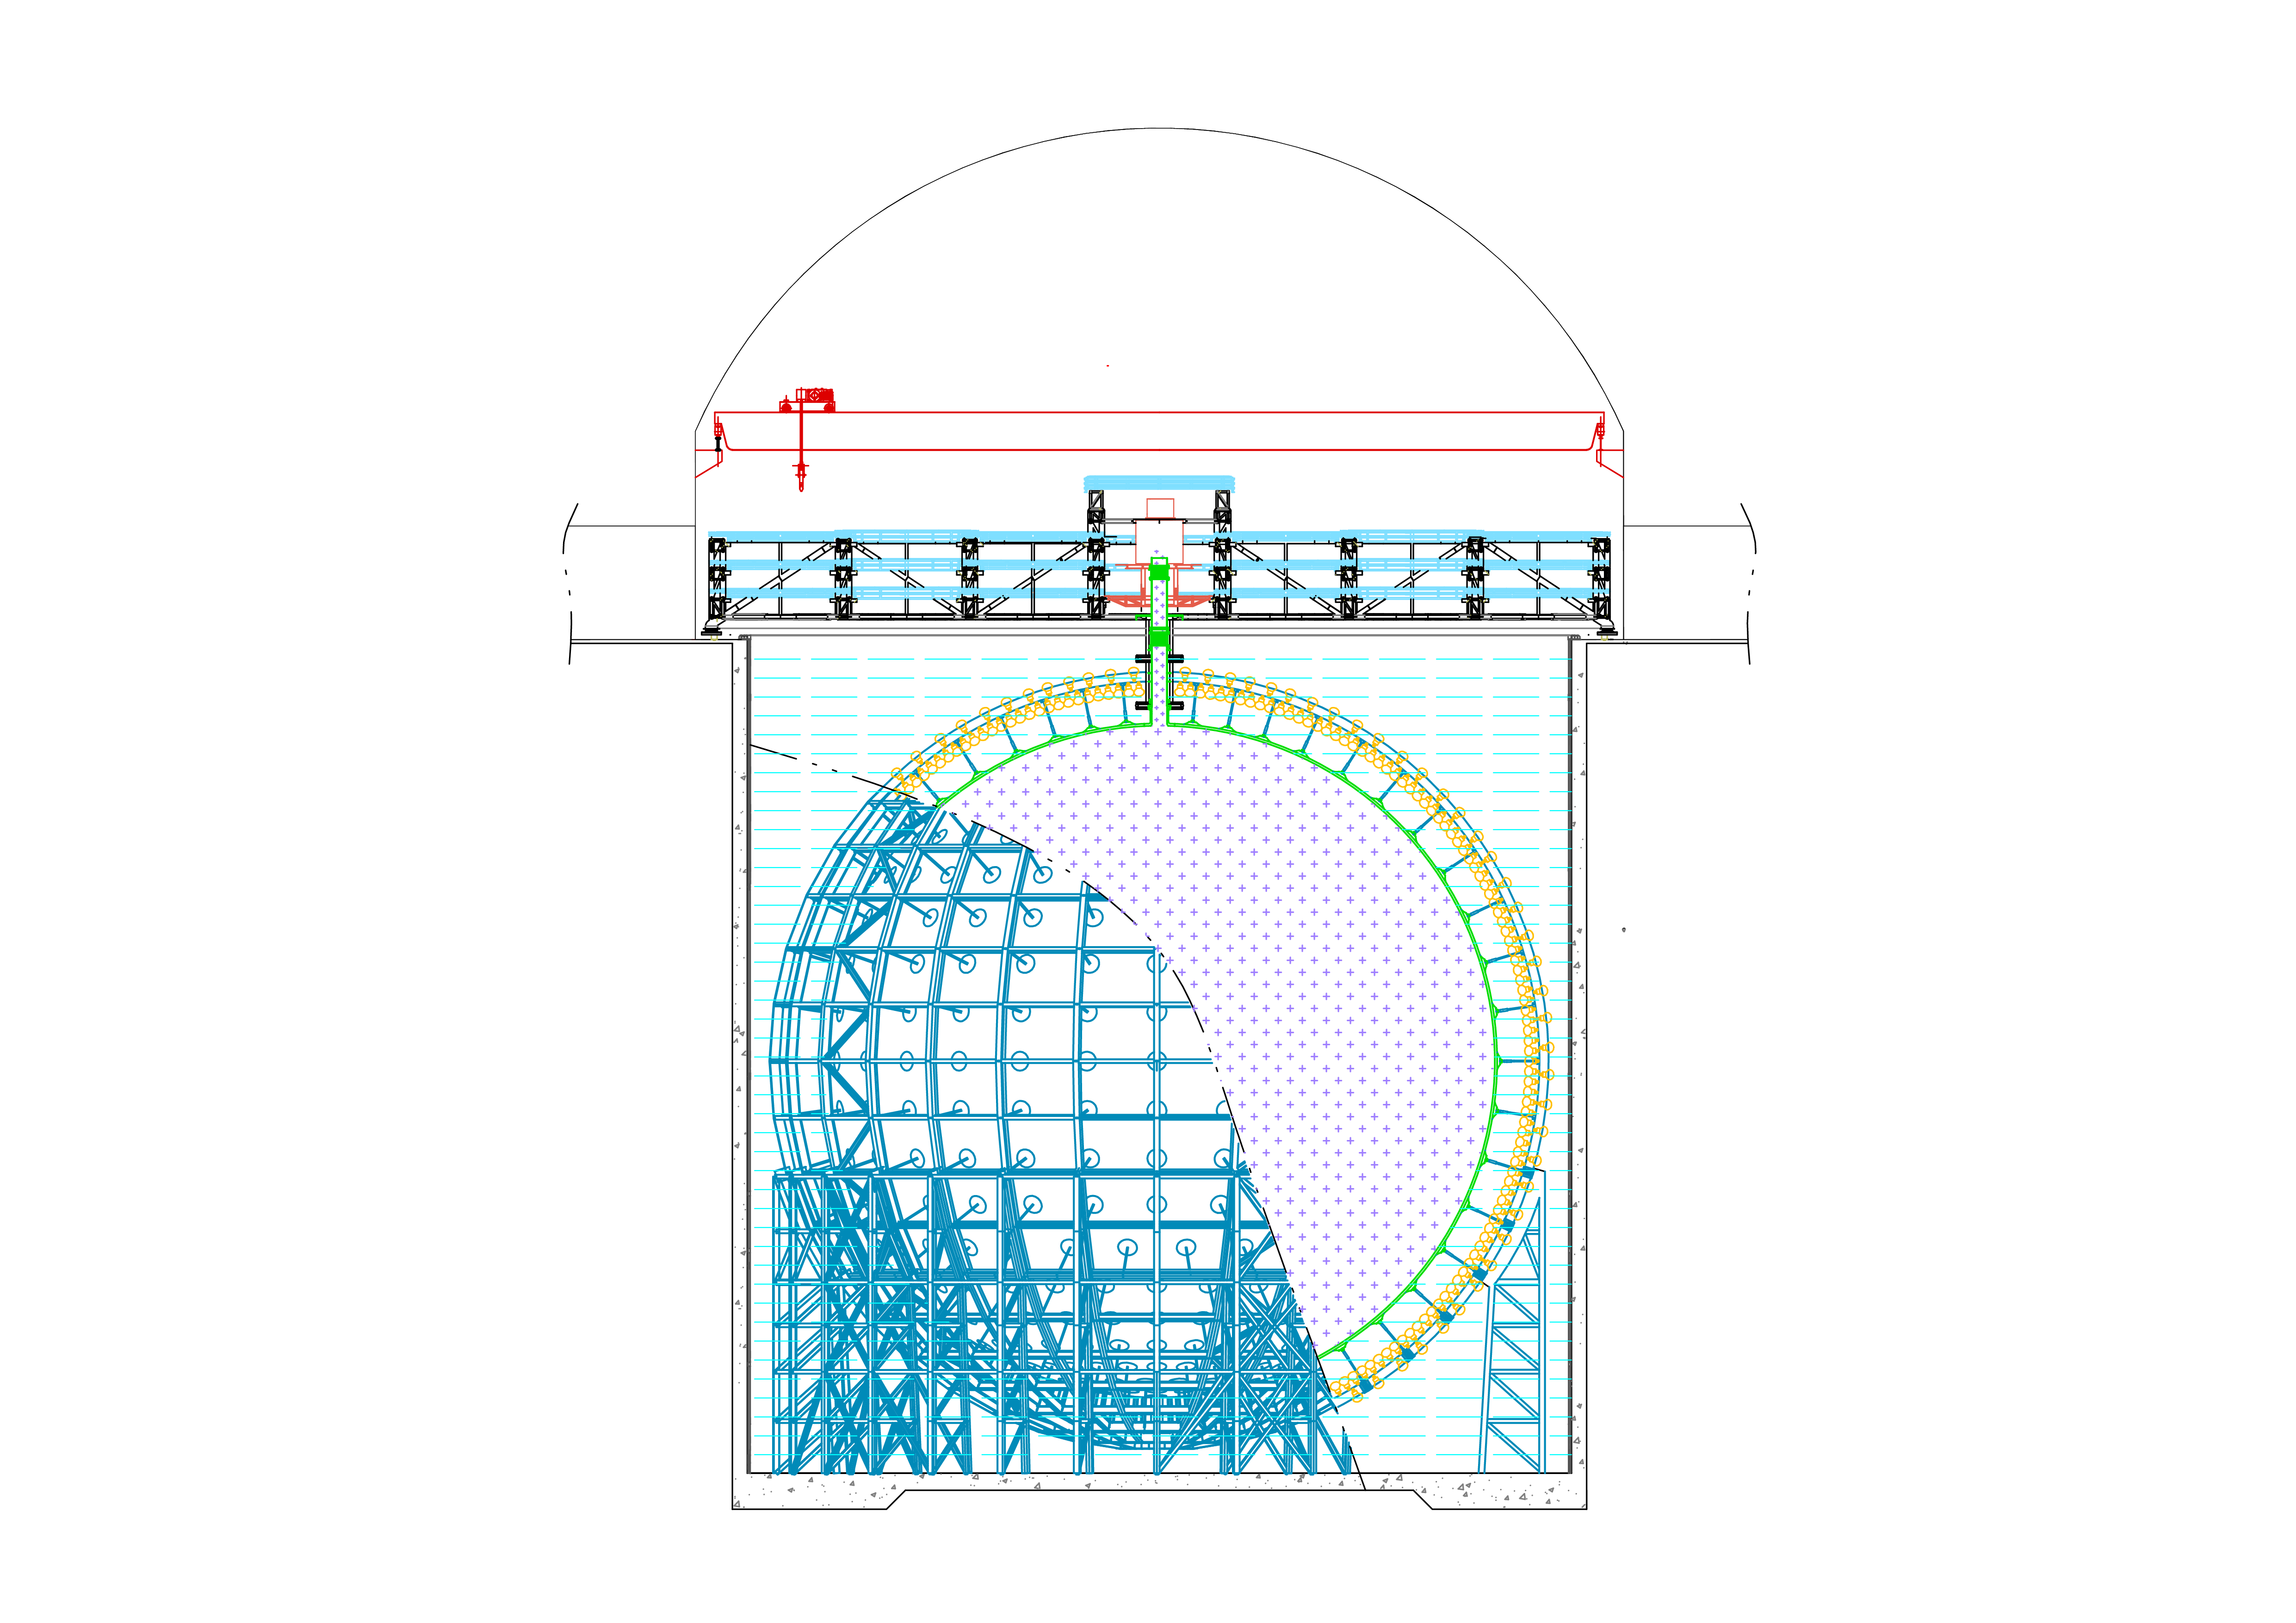
\includegraphics[height=6cm]{images/juno/drawing_schema.png}
    \caption{Schematics view of the JUNO detector.}
    \label{fig:juno:juno-schema}
  \end{subfigure}
  \hfill
  \begin{subfigure}[b]{0.45\textwidth}
    \centering
    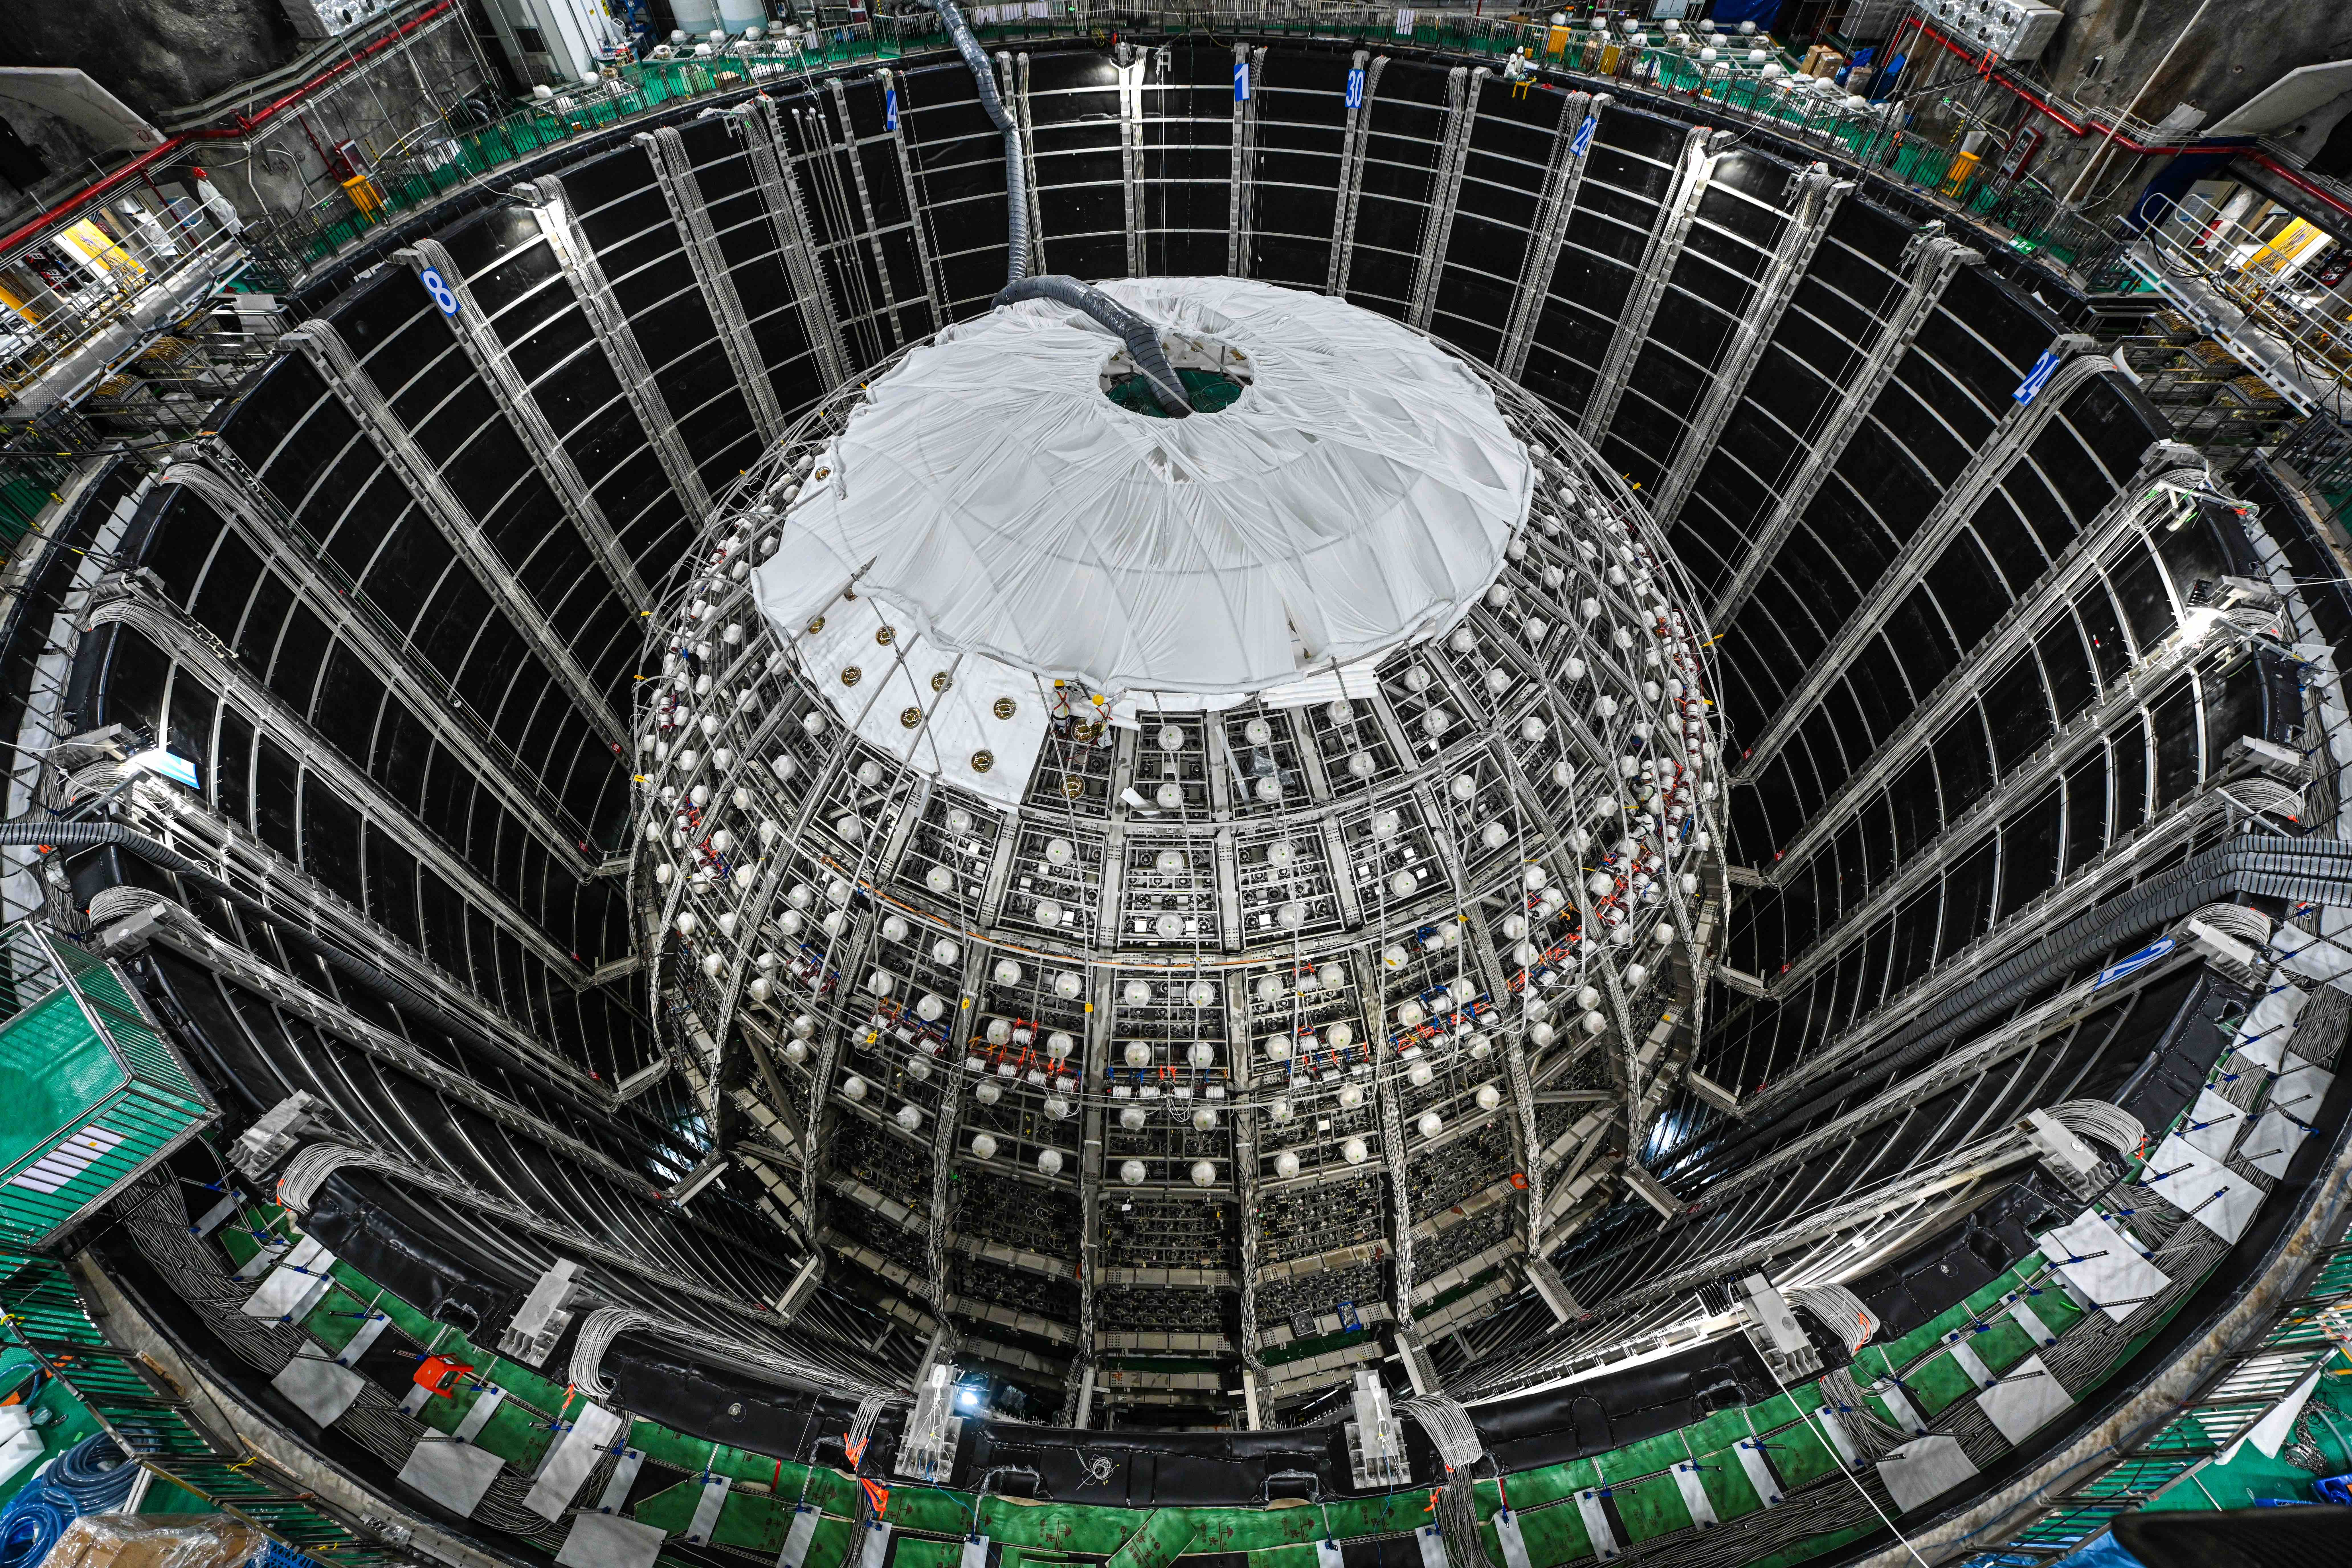
\includegraphics[height=4cm]{images/juno/top_down_view.jpg}
    \caption{Top down view of the JUNO detector under construction}
  \end{subfigure}
  \caption{}
\end{figure}

This section cover in details the different components of the detector and the detection systems.

\subsection{Detection principle}
\label{sec:juno:detct}

The CD will detect the neutrino and measure their energy mainly via an Inverse Beta Decay (IBD) interaction with proton mainly from the $^{12}$C and H nucleus in the LS:
\begin{equation*}
  \bar{\nu}_e + p \rightarrow n + e^+
\end{equation*}
Kinematics calculation shows that this interaction has an energy threshold for the $\bar{\nu}_e$ of $ (m_n + m_e - m_p ) \approx 1.806 ~ \mathrm{MeV}$ \cite{strumia_precise_2003}.
This threshold make the experiment blind to very low energy neutrinos. The residual energy $E_{\nu} - 1.806 ~ \mathrm{MeV}$ is be distributed as kinetic energy between the positron and the neutron.
The energy of the emitted positron $E_e$ is given by \cite{strumia_precise_2003}
\begin{equation}
  E_e = \frac{(E_\nu - \delta)(1+\epsilon_\nu) + \epsilon_\nu \cos \theta \sqrt{(E_\nu - \delta)^2 + \kappa m_e^2}}{\kappa}
\end{equation}
where $\kappa = (1 + \epsilon_\nu)^2 - \epsilon_\nu^2 \cos^2 \theta \approx 1$, $\epsilon_\nu = \frac{E_\nu}{m_p} \ll 1$ and $\delta = \frac{m_n^2 - m_p^2 - m_e^2}{2m_p} \ll 1$.
We can see from this equation that the positron energy is strongly correlated to the neutrino energy.


The positron and the neutron will then propagate in the detection medium, the Liquid Scintillator (LS), loosing their kinetic energy by exciting the molecule of the LS (more details in Section \ref{sec:juno:LS}). Once stopped, the positron will annihilate with an electron from the medium producing two 511 KeV gamma. Those gamma will themselves interact with the LS, exciting it before being absorbed by photoelectrical effect. The neutron will be captured by an hydrogen, emitting a 2.2 MeV gamma in the process. This gamma will also deposit its energy before being absorbed by the LS.

\begin{figure}[ht]
  \centering
  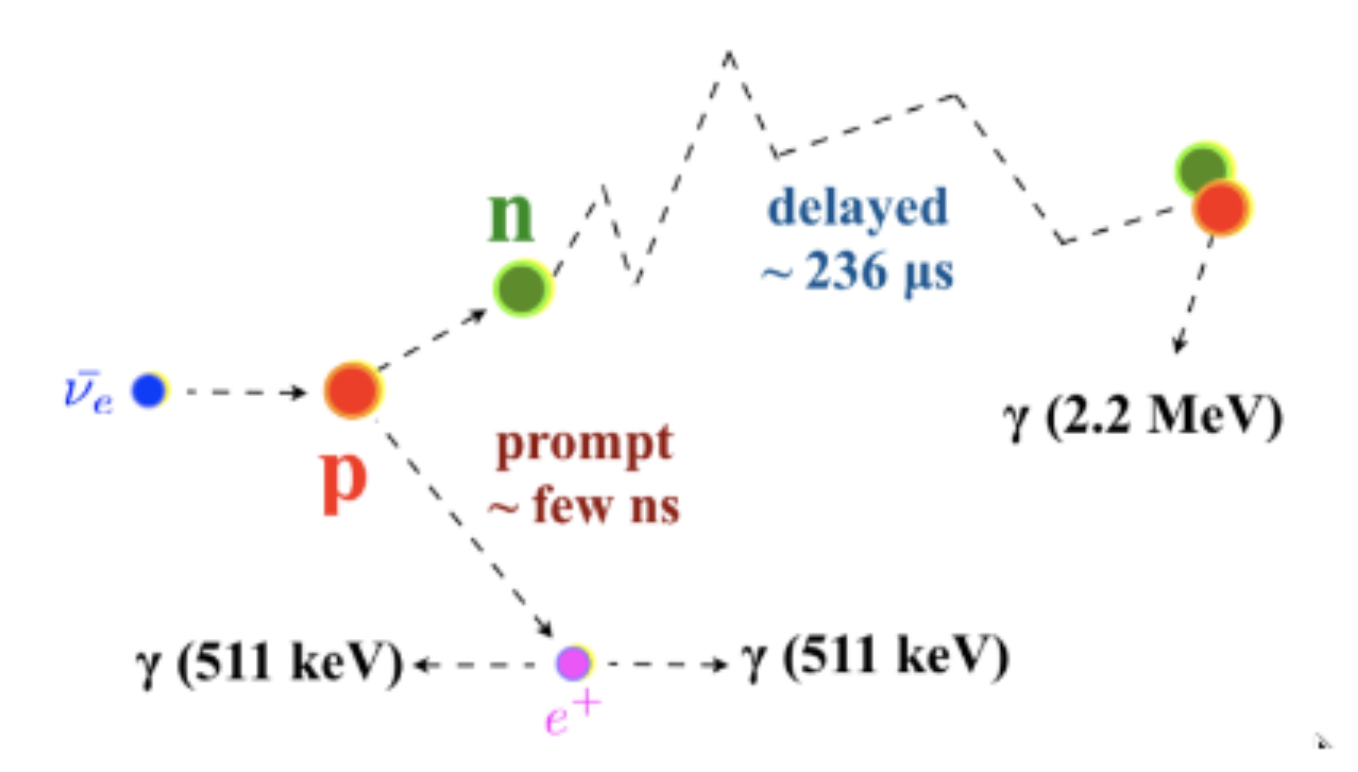
\includegraphics[width=8cm]{images/juno/IDB-JUNO.png}
  \caption{Schematics of an IBD interaction in the central detector of JUNO}
  \label{fig:juno:IBD}
\end{figure}

The scintillation photons have frequency in the UV and will propagate in the LS, being re-absorbed and re-emitted by compton effect before finally be captured by PMTs instrumenting the acrylic sphere. The analog signal of the PMTs digitized by the electronic is the signal of our experiment. The signal produced by the positron is subsequently called the prompt signal, and the signal coming from the neutron the delayed signal. This naming convention come from the fact that the positron will deposit its energy rather quickly (few ns) where the neutron will take a bit more time ($\sim$ 236 $\mu$s).

\subsection{Central Detector (CD)}
\label{sec:juno:CD}

The central detector, composed of 20 ktons of Liquid Scintillator (LS), is the main part of JUNO. The LS is contained in a spherical acrylic vessel supported by a stainless steel structure. The CD and its structural support are submerged in a cylindrical water pool of 43.5m diameter and 44m height. We're confident that the water pool provide sufficient buffer protection in every direction against the rock radioactivity.
\subsubsection{Acrylic vessel}
The acrylic vessel is a spherical vessel of inner diameter of 35.4 m and a thickness of 120 mm. It is assembled from 265 acrylic panels, thermo bonded together. The acrylic recipes has been carefully tuned with extensive R\&D to ensure it does not include plasticizer and anti-UV material that would stop the scintillation photons.
Those panels requires to be pure of radioactive materials to not cause background. Current setup where the acrylic panels are molded in cleanrooms of class 10000, let us reach a uranium and thorium contamination of <0.5 ppt. The molding and thermoforming processes is optimized to increase the assemblage transparency in water to >96\%. The acrylic vessel is supported by a stainless steel structure via supporting node (fig \ref{fig:juno:sup_node}). The structure and the nodes are designed to be resilient to natural catastrophic events such as earthquake and can support many times the effective load of the acrylic vessel.

\begin{figure}[ht]
  \centering
  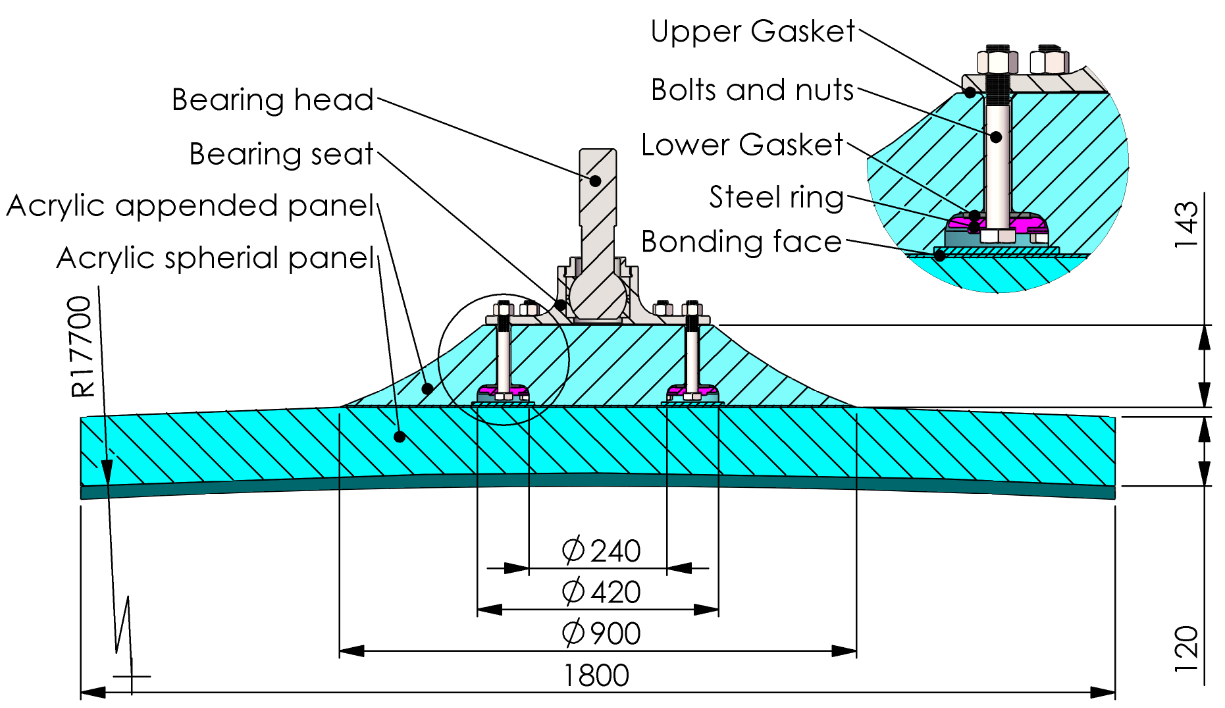
\includegraphics[height=4cm]{images/juno/node_b.png}
  \caption{Schematics of the supporting node for the acrylic vessel}
  \label{fig:juno:sup_node}
\end{figure}

\subsubsection{Liquid scintillator}
\label{sec:juno:LS}

The Liquid Scintillator (LS) has a similar recipe as the one used in Daya Bay \cite{bay_optimization_2020} but without gadolinium doping. It is made of three components, necessary to shift the wavelength of emitted photons to prevent their reabsorption and to shift their wavelength to the PMT sensitivity region as illustrated in Figure \ref{fig:juno:LS_spectrum_and_PMT_sensitivity}:
\begin{enumerate}
  \item The detection medium, the \textit{linear alkylbenzene} (LAB). Selected because of its excellent transparency, high flash point, low chemical reactivity and good light yield. Accounting for $\sim 98\%$ of the LS, it is the main component with which ionizing particles and gamma interact. Charged particles will collide with its electronic cloud transferring energy to the molecules, gamma will interact via compton effect with the electronic cloud before finally be absorbed via photoelectric effect.
  \item The second component of the LS is the \textit{2,5-diphenyloxazole} (PPO). A fraction of the excitation energy of the LAB is transferred to the PPO, mainly via non radiative process \cite{birks_chapter_1964}. The PPO molecules de-excites in the same way, transferring their energy to the bis-MSB. The PPO makes for $~1.5$ \% of the LS.
  \item The last component is the \textit{p-bis(o-methylstyryl)-benzene} (bis-MSB). Once excited by the PPO, it will emit photon with an average wavelength of $\sim430$ nm (full spectrum in Figure \ref{fig:juno:LS_spectrum_and_PMT_sensitivity}) that can thus be detected by our photo-multipliers systems. It amount for $\sim 0.5$\% of the LS.
\end{enumerate}

\begin{figure}[ht]
  \centering
  \begin{subfigure}[b]{0.48\textwidth}
    \centering
    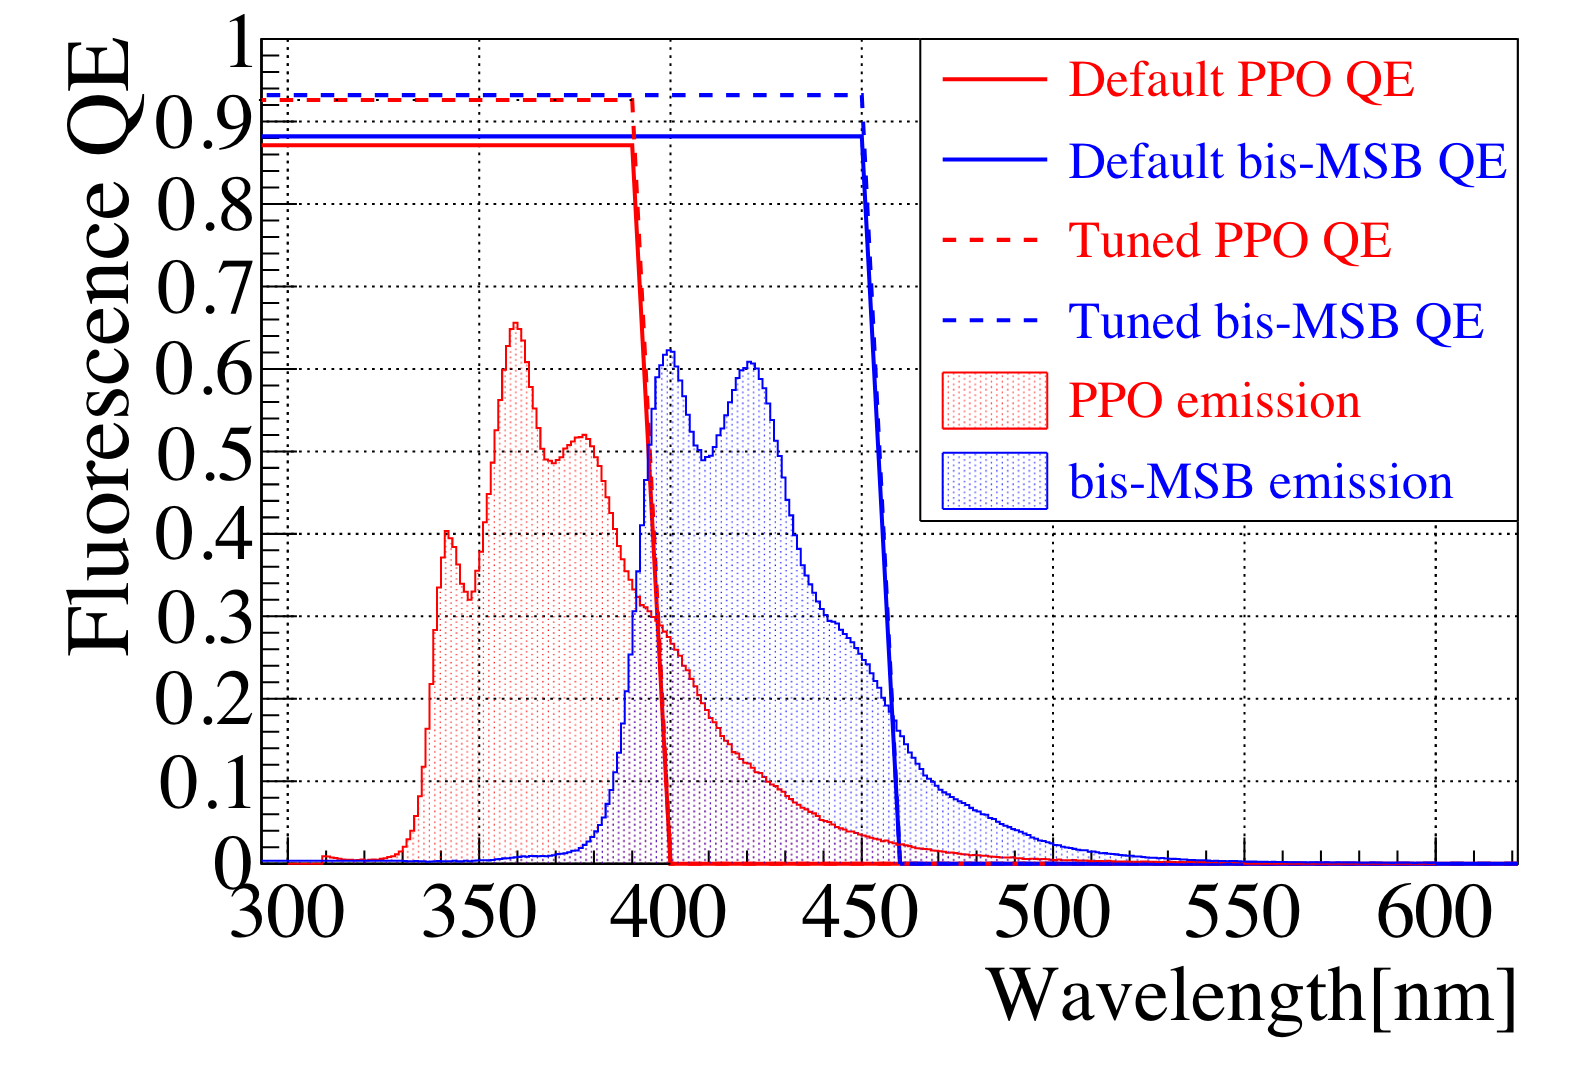
\includegraphics[height=5cm]{images/juno/LS_spectrum.png}
  \end{subfigure}
  \hfill
  \begin{subfigure}[b]{0.48\textwidth}
    \centering
    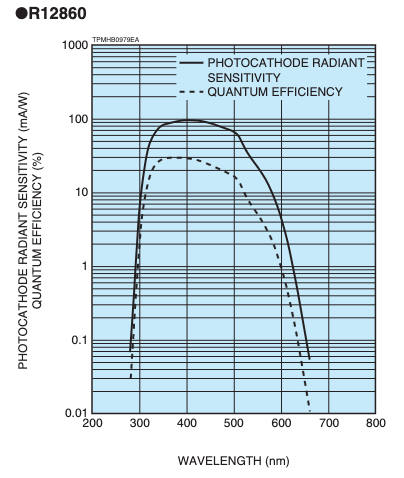
\includegraphics[height=5cm]{images/juno/LPMT_efficiency.png}
  \end{subfigure}
  \caption{\textbf{On the left:} Quantum efficiency (QE) and emission spectrum of the LAB and the bis-MSB \cite{bay_optimization_2020}. \textbf{On the right:} Sensitivity of the Hamamatsu LPMT depending on the wavelength of the incident photons \cite{noauthor_photomultiplier_nodate}.}
  \label{fig:juno:LS_spectrum_and_PMT_sensitivity}
\end{figure}

This formula has been optimized using dedicated studies with a Daya Bay detector \cite{bay_optimization_2020, zhang_complete_2020} to reach the requirements for the JUNO experiment:
\begin{itemize}
  \item A light yield / MeV of the amount of $10^4$ photons to maximize the statistic in the energy measurement.
  \item An attenuation length comparable to the size of the detector to prevent losing photons during their propagation in the LS. The final attenuation length is 25.8m \cite{yang_light_2017} to compare with the CD diameter of 35.4m.
  \item Uranium/Thorium radiopurity to prevent background signal. The reactor neutrino program require a contamination fraction $F<10^{-15}$ while the solar neutrino program require $F<10^{-17}$.
\end{itemize}

The LS will frequently be purified and tested in the Online Scintillator Internal Radioactivity Investigation System (OSIRIS) \cite{juno_collaboration_design_2021} to ensure that the requirements are kept during the lifetime of the experiment, more details to be found in Section \ref{sec:juno:OSIRIS}.

\subsubsection{Large Photo-Multipliers Tubes (LPMTs)}
\label{sec:juno:LPMT}

The scintillation light produced by the LS is then collected by Photo-Multipliers Tubes (PMT) that transform the incoming photon into an electric signal. As described in Figure \ref{fig:juno:pmt-schem}, the incident photons interact with the photocatode via photoelectric effect producing an electron called a Photo-Electron (PE). This PE is then focused on the dynodes where the high voltage will allow it to be multiplied. After multiple amplification the resulting charge - in coulomb [C] - is collected by the anode and the resulting electric signal can be digitalized by the readout electronics from which the charge and timing can be extracted.

\begin{figure}[ht]
  \centering
  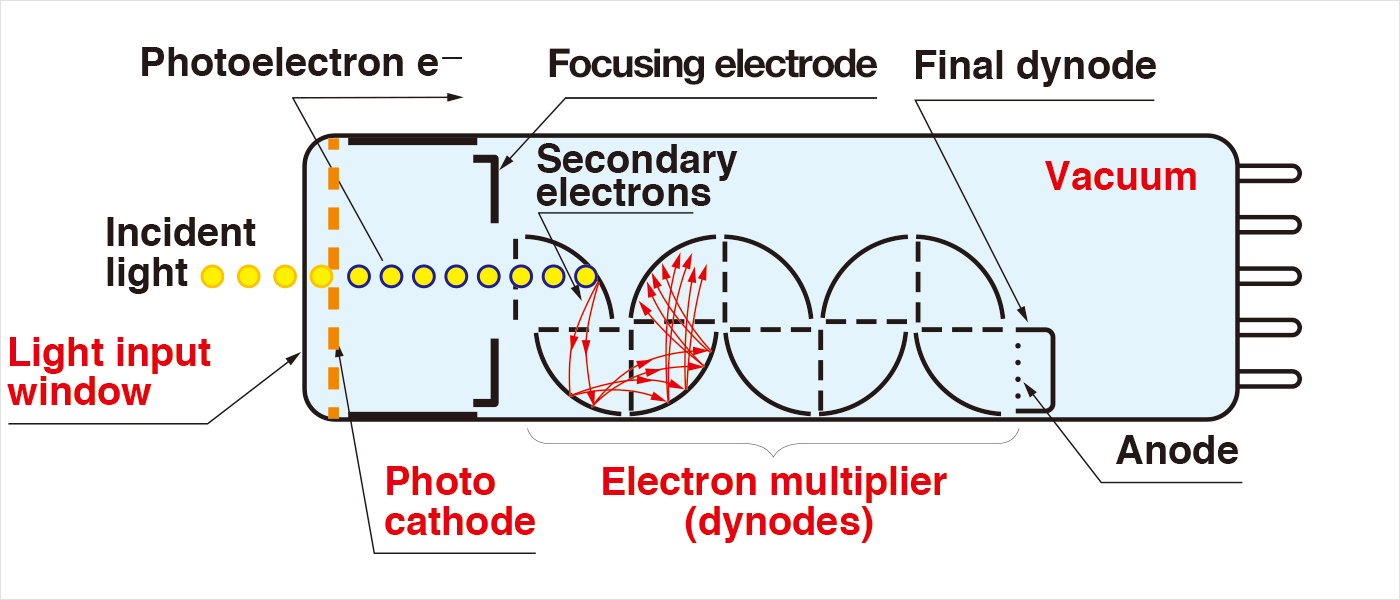
\includegraphics[height=4cm]{images/juno/pmt_schematic.png}
  \caption{Schematic of a PMT}
  \label{fig:juno:pmt-schem}
\end{figure}

The Large Photo-Multipliers Tubes (LPMT), used in the central detector and in the water pool, are 20-inch (50.8 cm) radius PMTs. $\sim 5000$ dynode-PMTs \cite{noauthor_photomultiplier_nodate} were produced by the Hamamatsu$^{\copyright}$ company and $\sim 15000$ Micro-Channel Plate (MCP) \cite{abusleme_mass_2022} by the NNVT$^{\copyright}$ company. This system is the one responsible for the energy measurement with a energy resolution of $3\%/\sqrt{E}$, resolution necessary for the mass ordering measurement. To reach this precision, the system is composed of 17612 PMTs quasi uniformly distributed over the detector for a coverage of 75.2\% reaching $\sim 1800$ PE/MeV or $\sim 2.3 \%$ resolution due to statistic, leaving $\sim 0.7\%$ for the systematic uncertainties. They are located outside the acrylic sphere in the water pool facing the center of the detector.
To maintain the resolution over the lifetime of the experiment, JUNO require a failure rate < 1\% over 6 years.

The LPMTs electronic are divided in two parts. One "near", located underwater, in proximity of the LPMT to reduce the cable length between the PMT and early electronic. A second one, outside of the detector that is responsible for higher level analysis before sending the data to the DAQ.

The light yield per MeV induce that a LPMT can collect between 1 and 1000 PE per event, a wide dynamic range,  causing non linearity in the PMT response that need to be understood and calibrated, see Section \ref{sec:juno:calib} for more details.

Before performng analysis, the analog readout of the LPMT need to be amplified, digitised and packaged by the readout electronics schematized in Figure \ref{fig:juno:lpmt_elec}. This electronic is splitted in two parts: \textit{wet} electronic that are located near the LPMTs, protected in an Underwater Box (UWB) and the \textit{dry} electronics located in deicated rooms outside of the water pool.

The LPMTs are connected to the UWB by groups of three. Each UWB contains:
\begin{itemize}
  \item Three high voltage units, each one powering a PMT.
  \item A global control unit, responsible for the digitization of the waveform, composed of six analog-digital units that produce digitized waveform and a Field Programmable Gate Array (FPGA) that complete the waveform with metadatas such as the local timestamp trigger, etc... Ths FPGA also act as a data buffer when needed by the DAQ and trigger system.
  \item Additional memory in order to temporally store the data in case of sudden burst of the input rate (such as in the case of nearby supernovae).
\end{itemize}

\begin{figure}[ht]
  \centering
  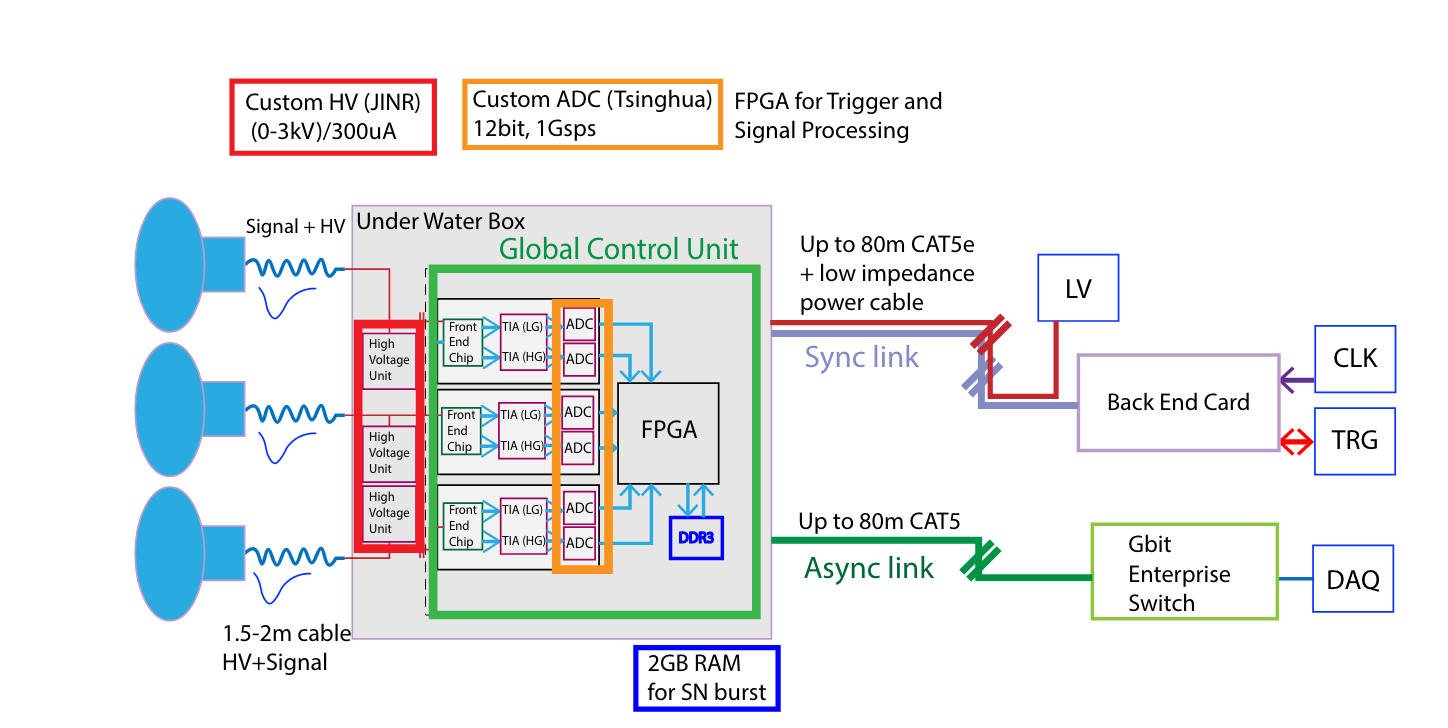
\includegraphics[height=6cm]{images/juno/LPMT_readout.png}
  \caption{The LPMT electronics scheme. It is composed of two part, the \textit{wet} electronics on the left, located underwater and the \textit{dry} electronics on the right. They are connected by Ethernet cable for data transmission and a dedicated low impedance cable for power distribution}
  \label{fig:juno:lpmt_elec}
\end{figure}

The \textit{dry} electronic synchronize the signals from the UWBs abd centralise the information of the CD LPMTs. It act as the Global Trigger by sending the UWB data to DAQ in the case if the LPMT multiplicity condition is fulfilled.


\subsubsection{Small Photo-Multipliers Tubes (SPMTs)}
\label{sec:juno:SPMT}

The Small PMT (SPMTs) system is made of 3-inch (7.62 cm) PMTs. They will be used in the CD as a secondary detection system. Those 25600 SPMTs will observe the same events as the LPMTs, thus sharing the physics and detector systematics up until the photon conversion. With a detector coverage of 2.7\%, this system will collect $\sim 43$ PE/MeV for a final energy resolution of $\sim 17\%$. This resolution is not enough to measure the NMO, $\theta_{13}$, $\Delta m^2_{31}$ but will be sufficient to independently measure $\theta_{12}$ and $\Delta m^2_{21}$.

The benefit of this second system is to be able to perform another, independent measure of the same events as the LPMTs, constituing the Dual Calorimetry useful for calibrationa and, as it we will explore in this thesis, for physics analysis.
Due to the low PE rate, SPMTs will be running in photo-counting mode in the reactor range and thus will be insensitive to LPMT intrisic effect (see Section \ref{sec:juno:calib}). Using this property, the intrinsic charge non linearity of the LPMTs can be measured by comparing the PE count in the SPMTs and LPMTs \cite{han_dual_2021}. Also, due to their smaller size and electronics, SPMTs have a better timing resolutions than the LPMTs.
At higher energy range, like supernovae events, LPMTs will saturate where SPMTs due to their lower PE collection will to produce a reliable measure of the energy spectrum.

The SPMTs will be grouped by pack of 128 to an UWB hosting their electronics as illustrated in Figure \ref{fig:juno:spmt_elec}. This underwater box host two high voltage splitter boards, each one supplying 64 SPMTs, an ASIC Battery Card (ABC) and a global control unit.

The ABC board will readout and digitize the charge and time of the 128 SPMTs signals and a FPGA will joint the different metadata. The global control unit will handle the powering and control of the board and will be in charge of the transmition of the data to the DAQ.

\begin{figure}[ht]
  \centering
  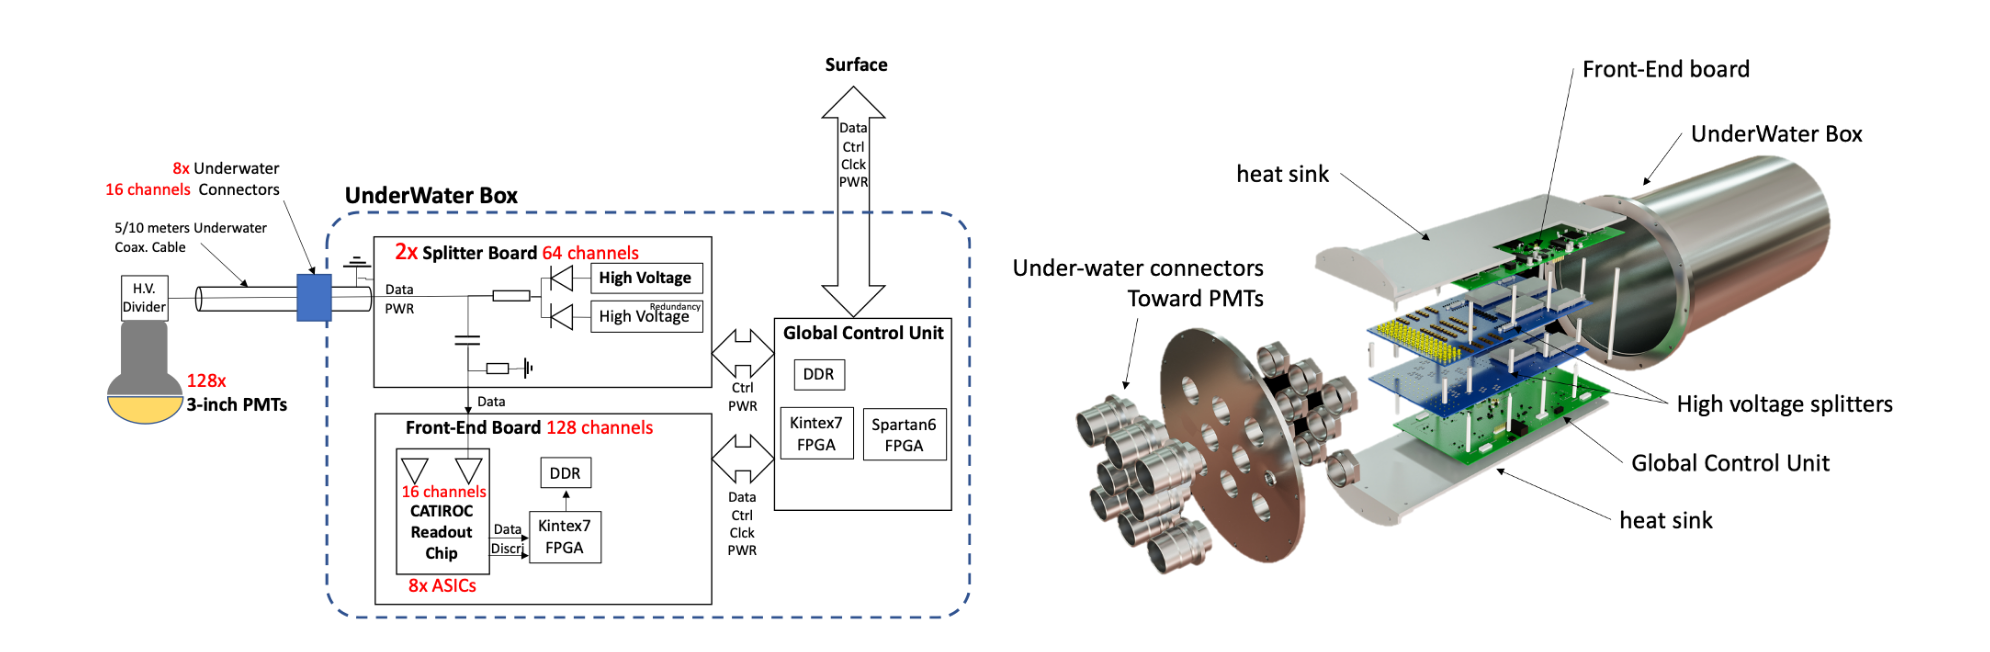
\includegraphics[height=6cm]{images/juno/SPMT_readout.png}
  \caption{Schematic of the JUNO SPMT electronic system (\textbf{left}), and exploded view of the main component of the UWB (\textbf{right})}
  \label{fig:juno:spmt_elec}
\end{figure}

\subsection{Veto detector}

The CD will be bathed in constant background noise coming from numerous sources : the radioactivity from surrounding rock and its own components or from the flux of cosmic muons. This background needs to be rejected to ensure the purity of the IBD spectrum. To prevent a big part of them, JUNO use two veto detector that will tag events as background before CD analysis.

\subsubsection{Cherenkov in water pool}

The Water Cherenkov Detector (WCD) is the instrumentation of the water buffer around the CD. When high speed charged particles will pass through the water, they will produced cherenkov photons. The light will be collected by 2400 MCP LPMTs installed on the outer surface of the CD structure. The  muons veto strategy is based on a PMT multiplicity condition. WCD PMTs are grouped in ten zones: 5 in the top, 5 in the bottom. A veto is raised either when more than 19 PMTs are triggered in one zone or when two adjacent zones simultaneously trigger more than 13 PMTs. Using this trigger, we expect to reach a muon detection efficiency of 99.5\% while keeping the noise at reasonable level.

\subsubsection{Top tracker}
The JUNO Top Tracker (TT) is a plastic scintillator detector located on the top of the experiment (see Figure \ref{fig:juno:tt}). Made from plastic scintillator from OPERA \cite{acquafredda_opera_2009} layered horizontally in 3 layers on the top of the detector, the TT will be able to detect incoming atmospheric muons.
With its coverage, about 1/3 of the of all atmospheric muons that passing through the CD will also pass through the 3 layer of the detector. While it does not cover the majority of the CD, the TT is particularly effective to detect muons coming through the filling chimney region which might present difficulties from the other subsystems in some classes of events.
\begin{figure}[ht]
  \centering
  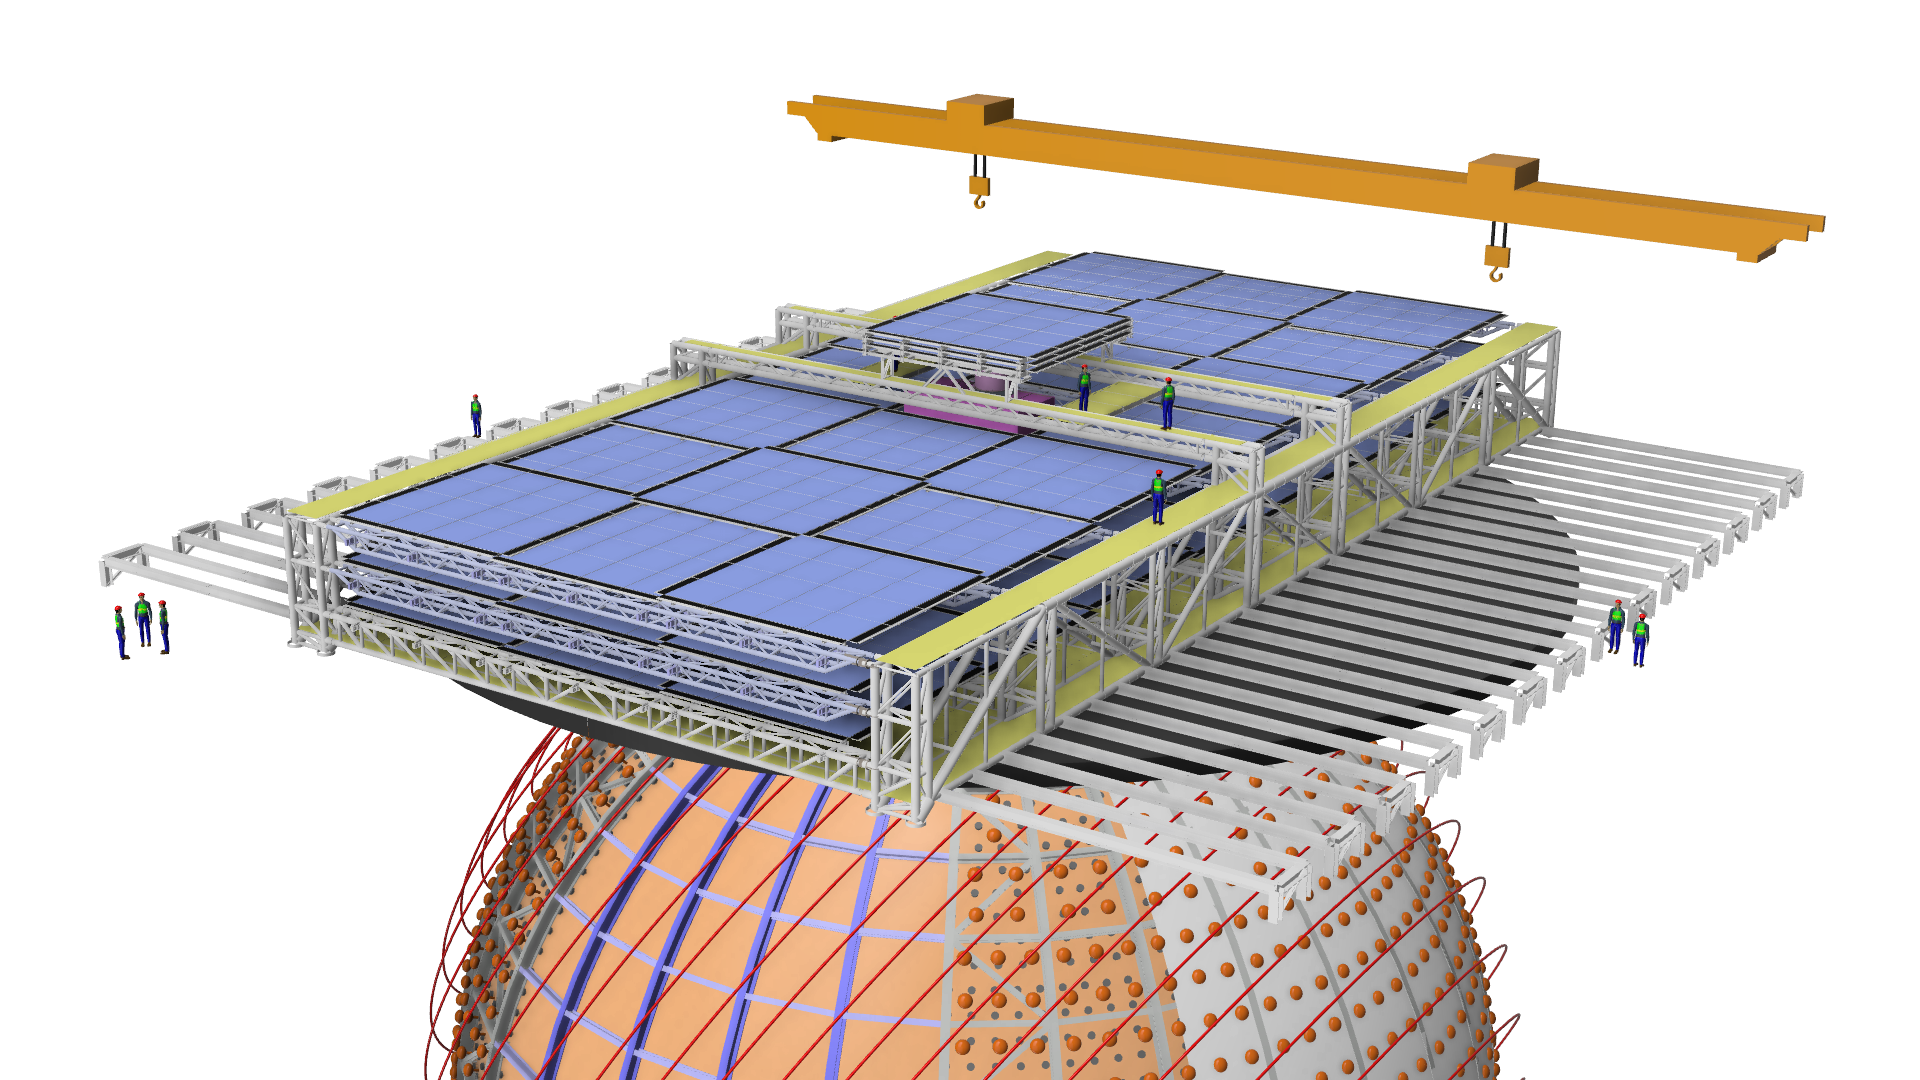
\includegraphics[height=5cm]{images/juno/Global_TT_01.png}
  \caption{The JUNO top tracker}
  \label{fig:juno:tt}
\end{figure}

\section{Calibration strategy}
\label{sec:juno:calib}

The calibration is a crucial part of the JUNO experiment. The detector will continuously bath in neutrinos coming from the close nuclear power plant, from other sources such as geo neutrinos, the sun and will be exposed to background noise coming from atmospheric muons and natural radioactivity.
Because of this continuous rate, low frequency signal event, we need high frequency, recognisable sources in the energy range of interest : [0-12] MeV for the positron signal and 2.2 MeV for the neutron capture.
It is expected that the CD response will be different depending on the type of particle, due to the interaction with LS, the position on the event and the optical response of the acrylic sphere (see Section \ref{sec:juno:reco}).
We also expect a non-linear energy response of the CD due to the LS properties \cite{bay_optimization_2020} but also due to the reponse of the LPMTs system when collecting a large amount of PE \cite{han_dual_2021}.

\subsection{Energy scale calibration}

While electrons and positrons sources would be ideal, for a large LS detector thin-walled electrons or positrons sources could lead to leakage of radionucleides causing radioactive contamination. Instead, we consider gamma sources in the range of the prompt energy of IBDs. The sources are reported in table \ref{tab:juno:calib_source}.

\begin{table}[ht]
  \centering
  \begin{tabular}{|c|c|c|}
    \hline
    Sources / Processes & Type & Radiation \\
    \hline
    $^{137}$Cs          & $\gamma$ & 0.0662 MeV \\
    $^{54}$Mn           & $\gamma$ & 0.835 MeV \\
    $^{60}$Co           & $\gamma$ & 1.173 + 1.333 MeV \\
    $^{40}$K            & $\gamma$ & 1.461 MeV \\
    $^{68}$Ge           & $e^{+}$  &  annihilation 0.511 + 0.511 MeV \\
    $^{241}$Am-Be       & $n,\gamma$ & neutron + 4.43 MeV (${12}$C*) \\
    $^{241}$Am-$^{13}$C & $n,\gamma$ & neutron + 6.13 MeV (${16}$O*) \\
    $(n, \gamma)p$      & $\gamma$ & 2.22 MeV \\
    $(n, \gamma)^{12}$C & $\gamma$ & 4.94 MeV or 3.68 + 1.26 MeV \\
    \hline
  \end{tabular}
  \caption{List of sources and their process considered for the energy scale calibration}
  \label{tab:juno:calib_source}
\end{table}

For the $^{68}$Ge source, it will decay in $^{68}$Ga via electron capture, which will itself $\beta^+$ decay into $^{68}$Zn. The positrons will be absorbed by the enclosure so only the annihilation gamma will be released. In addition, $(\alpha, n)$ sources like $^{241}$Am-Be and $^{241}$Am-$^{13}$C are used to provide both high energy gamma and neutrons, which will later be captured in the LS producing the 2.2 MeV gamma.

From this calibration we call $E_{vis}$ the "visible energy" that is reconstructed by our current algorithms and we compare it to the true energy deposited by the calibration source. The results shown in Figure \ref{fig:juno:nl} show the expected response of the detector from calibration sources. The non-linearity is clearly visible from the $E_{vis} / E_{true}$ shape. See \cite{juno_collaboration_calibration_2021} for more details.

\begin{figure}[ht]
  \centering
  \begin{subfigure}[b]{0.24\textwidth}
    \centering
    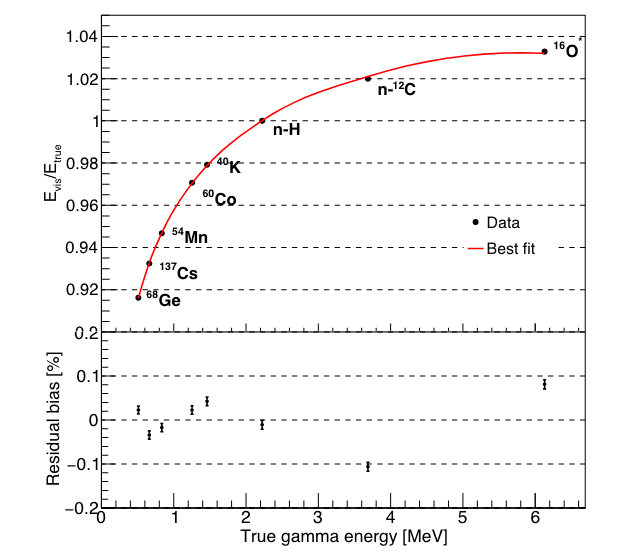
\includegraphics[width=\textwidth]{images/juno/gamma_nl.png}
    \caption{Gamma non-linearity}
    \label{fig:juno:nl:gamma}
  \end{subfigure}
  \begin{subfigure}[b]{0.37\textwidth}
    \centering
    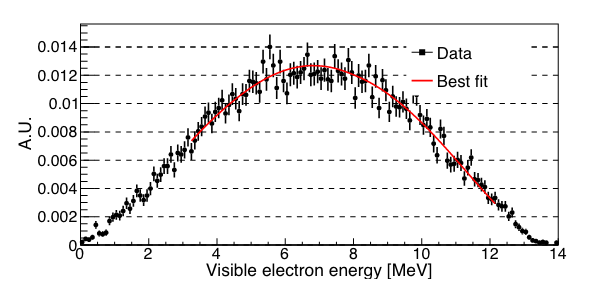
\includegraphics[width=\textwidth]{images/juno/boron_nl.png}
    \caption{Boron spectrum}
    \label{fig:juno:nl:boron}
  \end{subfigure}
  \begin{subfigure}[b]{0.37\textwidth}
    \centering
    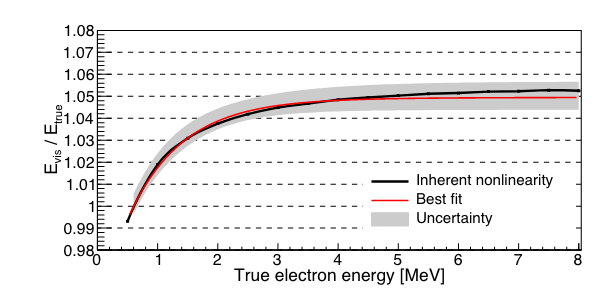
\includegraphics[width=\textwidth]{images/juno/e-_nl.png}
    \caption{Electron non-linearity}
    \label{fig:juno:nl:electron}
  \end{subfigure}
  \caption{Fitted and simulated non linearity of gamma, electron sources and from the $^{12}$B spectrum. Black points are simulated data. Red curves are the best fits. Figures taken from \cite{juno_collaboration_calibration_2021}.}
  \label{fig:juno:nl}
\end{figure}

\subsection{Calibration system}

The non-uniformity due to the event position in the detector (more details in Section \ref{sec:juno:reco}) will be studied using multiples systems that are schematized in Figure \ref{fig:juno:calib}. They allow to position sources at different location in the CD.

\begin{itemize}
  \item For a one-dimension vertical calibration, the Automatic Calibration Unit (ACU) will be able to deploy multiple radioactive sources or a pulse laser diffuser ball along the central axis of the CD through the top chimney. The source position precision is less than 1cm.
  \item For off-axis calibration, a calibration source attached to a Cable Loop System (CLS) can be moved on a vertical half-plane by adjusting the length of two connection cable. Two set of CSL will be deployed to provide a 79\% effective coverage of a vertical plane.
  \item A Guiding Tube (GT) will surround the CD to calibrate the non-uniformity of the response at the edge of the detector
  \item A Remotely Operated under-LS Vehicle (ROV) can be deployed to desired location inside LS for a more precise and comprehensive calibration. The ROV will also be equipped with a camera for inspection of the CD.
\end{itemize}

\begin{figure}[ht]
  \centering
  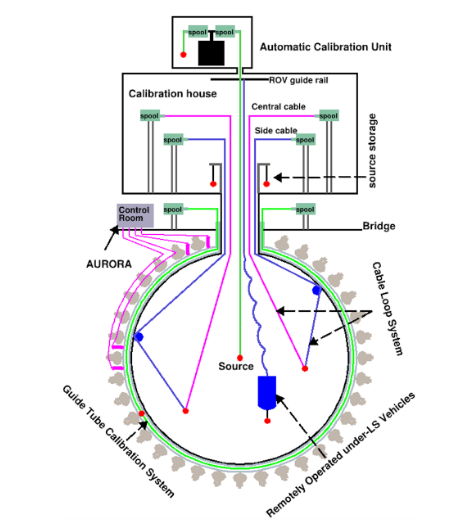
\includegraphics[height=6cm]{images/juno/calib.png}
  \caption{Overview of the calibration system}
  \label{fig:juno:calib}
\end{figure}

The preliminary calibration program is depicted in table \ref{tab:juno:calib_prog}.

\begin{table}[ht]
  \centering
  \begin{tabular}{c c c c}
    \hline
    Program & Purpose & System & Duration [min] \\
    \hline
    Weekly calibration & Neutron (Am-C) & ACU & 63 \\
                       & Laser & ACU & 78  \\
                       \hline
    Monthly calibration & Neutron (Am-C) & ACU & 120 \\
                        & Laser  & ACU  & 147 \\
                        & Neutron (Am-C) & CLS & 333 \\
                        & Neutron (Am-C) & GT  & 73  \\
                        \hline
    Comprehensive calibration & Neutron (Am-C) & ACU, CLS and GT & 1942 \\
                              & Neutron (Am-Be) & ACU & 75 \\
                              & Laser & ACU & 391 \\
                              & $^{68}$Ge & ACU & 75 \\
                              & $^{137}$Cs & ACU & 75 \\
                              & $^{54}$Mn & ACU & 75 \\
                              & $^{60}$Co & ACU & 75 \\
                              & $^{40}$K & ACU & 158 \\
    \hline
  \end{tabular}
  \caption{Calibration program of the JUNO experiment}
  \label{tab:juno:calib_prog}
\end{table}

\subsection{Instrumental non-linearity calibration}
\label{sec:juno:instr_nl}

One of the main interests of Dual Calorimetry is to calibrate away an instrumental effect called charge non linearity (QNL), which will be described in more detail in Chapter \ref{sec:joint_fit}.

In short, during a typical IBD event, between 0 and 100 PEs can be produced in a given LPMT (depending on the position of the interaction and the positron energy). This is a large dynamic range. When the number of PEs is high, the reconstruction of the LPMT charge can become inaccurate, underestimating the actual number of PEs as illustrated in Figure \ref{fig:juno:instr_nl}. This QNL is difficult to separate from other non linearities (like the non linearity in the LS photon yield as a function of the deposit energy). In chapter 5 and 6 of this thesis \cite{han_dual_2021}, a calibration method that constitutes the core of dual calorimetry are described.  They are based on the comparisons between signals seen in LPMTs and signals seen in SPMTs. In the latter system, due to its small angular  coverage, individual SPMT rarely see more than 1 PE per event, and therefore are essentially immune  against QNL. The method described in \cite{han_dual_2021} uses a tunable light source covering the range of 0 to 100 PE perLPMT channel

\begin{figure}[ht]
  \centering
  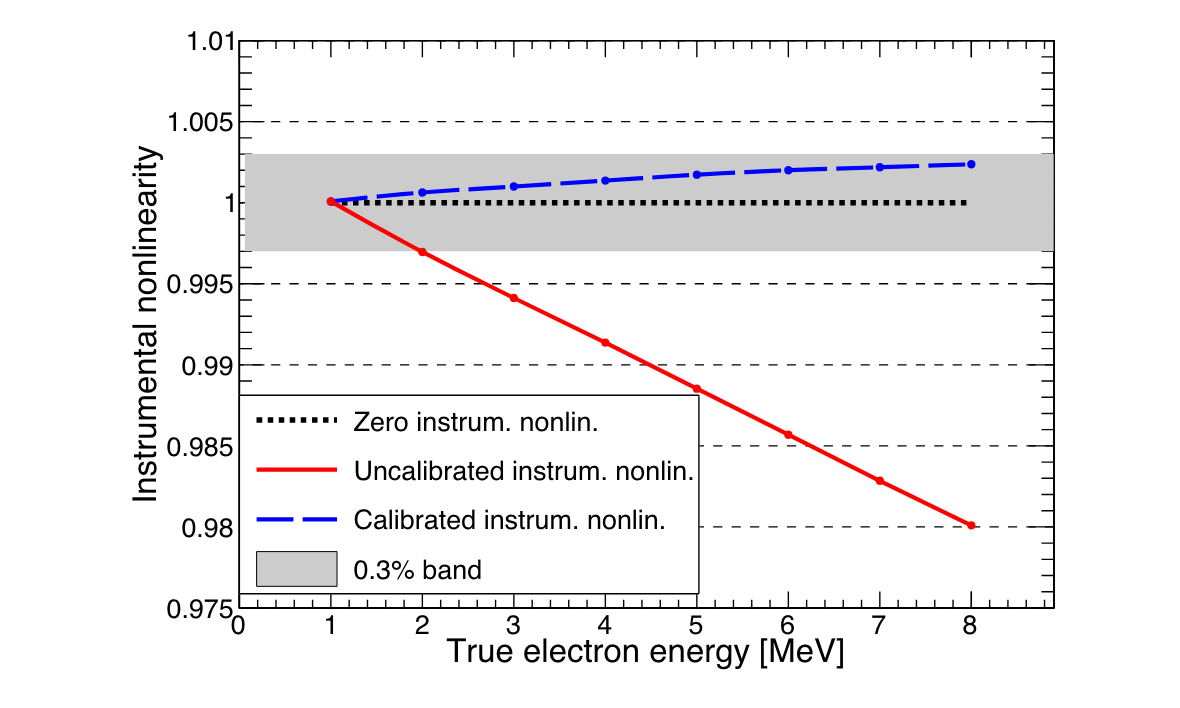
\includegraphics[height=6cm]{images/juno/instr_non_linearity.png}
  \caption{Event-level instrumental non-linearity, defined as the ratio of the total measured LPMT charge to the true charge for events at the center of the detector. The solid red line represents event-level non-linearity without the channel-level correction in an extreme hypothetical scenario of 50\% non-linearity over 100 PEs for the LPMTs. The dashed blue line represents that after the channel-level correction. The gray band shows the residual uncertainty of 0.3\%, after the channel-level correction. Figure taken from \cite{juno_collaboration_calibration_2021}.}
  \label{fig:juno:instr_nl}
\end{figure}


\section{Satellite detectors}
As introduced in Section \ref{sec:juno:nu_e_flux} and section \ref{sec:juno:LS}, the precise knowledge and understanding of the detector condition is crucial for the measurements of the NMO and oscillation parameters. Thus two satellite detectors will be setup to monitor the experiment condition. TAO to monitor and understand the $\bar{\nu}_e$ flux and spectrum coming from the nuclear reactor and OSIRIS to monitor the LS response.

\subsection{TAO}
\label{sec:juno:tao}
The Taishan Antineutrino Observatory (TAO) \cite{juno_collaboration_tao_2020, steiger_tao_2022} is a ton-level gadolinium doped liquid scintillator detector that will be located near the Taishan-1 reactor. It aim to measure the $\bar{\nu}_e$ spectrum at very low distance (44m) from the reactor to measure a quasi-unoscillated spectrum. TAO also aim to provide a major contribution to the so-called reactor anomaly \cite{mention_reactor_2011}. Its requirement are to the level of 2 \% energy resolution at 1 MeV.

\subsubsection{Detector}

The TAO detector is close, in concept, to the CD of JUNO. It is composed of an acrylic vessel containing 2.8 tons of gadolinium-loaded LS instrumented by an array of silicon photomultipliers (SiPM) reaching a 95\% coverage. To efficiently reduce the dark count of those sensors, the detector is cooled to -50 \textcelsius.
The $\bar{\nu}_e$ will interact with the LS via IBD, producing scintillation light, that will be detected by the SiPMs. From this signal the $\bar{\nu}_e$ energy and the full spectrum reconstructed.
This spectrum will then be used by JUNO to calibrate the unoscillated spectrum, most notably the fission product fraction that impact the rate and shape of the spectrum. A schema of the detector is presented in Figure \ref{fig:juno:tao}.

\subsection{OSIRIS}
\label{sec:juno:OSIRIS}
The Online Scintillator Internal Radioactivity Investigation System (OSIRIS) \cite{juno_collaboration_design_2021} is an ultralow background, 20 m$^3$ LS detector that will be located in JUNO cavern. It aim to monitor the radioactive contamination, purity and overall response of the LS before it is injected in JUNO.
OSIRIS will be located at the end of the purification chain of JUNO, monitoring that the purified LS meet the JUNO requirements. The setup is optimized to detect the fast coincidences decay of $^{214}\mathrm{Bi}-^{214}\mathrm{Po}$ and $^{212}\mathrm{Bi}-^{212}\mathrm{Po}$, indicators of the decay chains of U and Th respectively.
\subsubsection{Detector}
OSIRIS is composed of an acrylic vessel that will contains 17t of LS. The LS is instrumented by a PMT array of 64 20 inch PMTs on the top and the side of the vessel. To reach the necessary background level required by the LS purity measurements, in addition to being 700m underground in the experiment cavern, the acrylic vessel is immersed in a tank of ultra pure water. The water is itself instrumented by another array of 20 inch PMTs, acting as muon veto. A schema of the detector is presented in Figure \ref{fig:juno:osiris}.

\begin{figure}[ht]
  \centering
  \begin{subfigure}[t]{0.49\linewidth}
    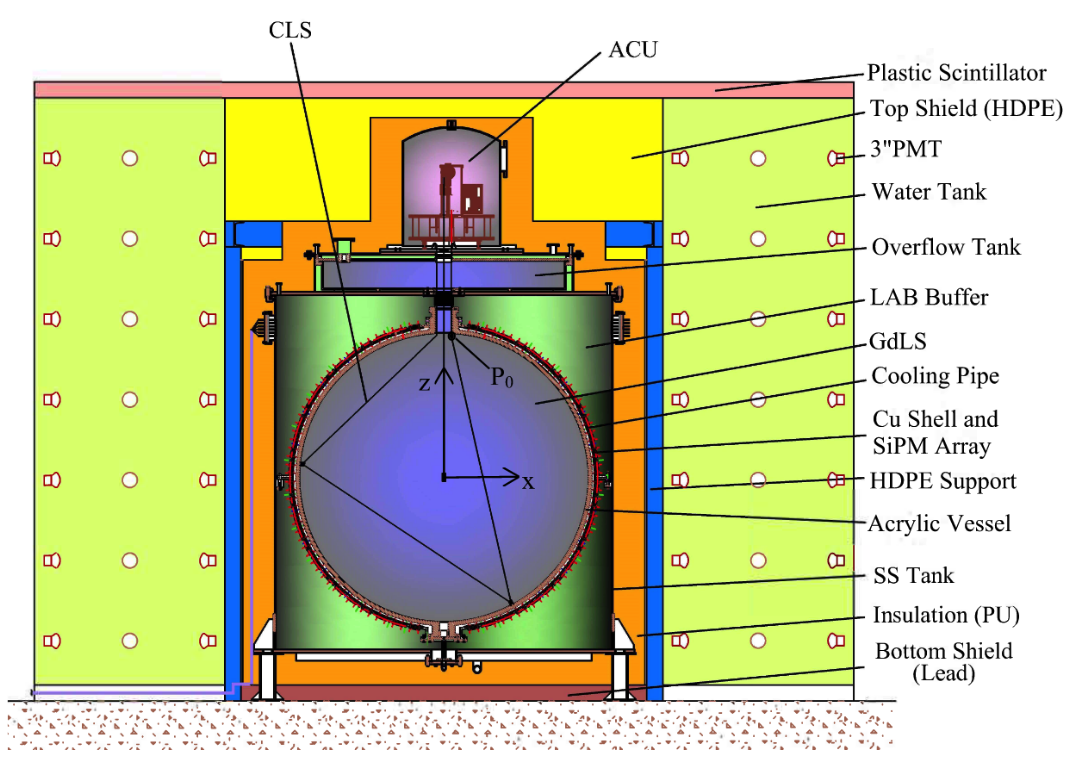
\includegraphics[width=\linewidth]{images/juno/tao_schematic.png}
    \caption{Schematic of the TAO satellite detector}
    \label{fig:juno:tao}
  \end{subfigure}
  \hfill
  \begin{subfigure}[t]{0.49\linewidth}
    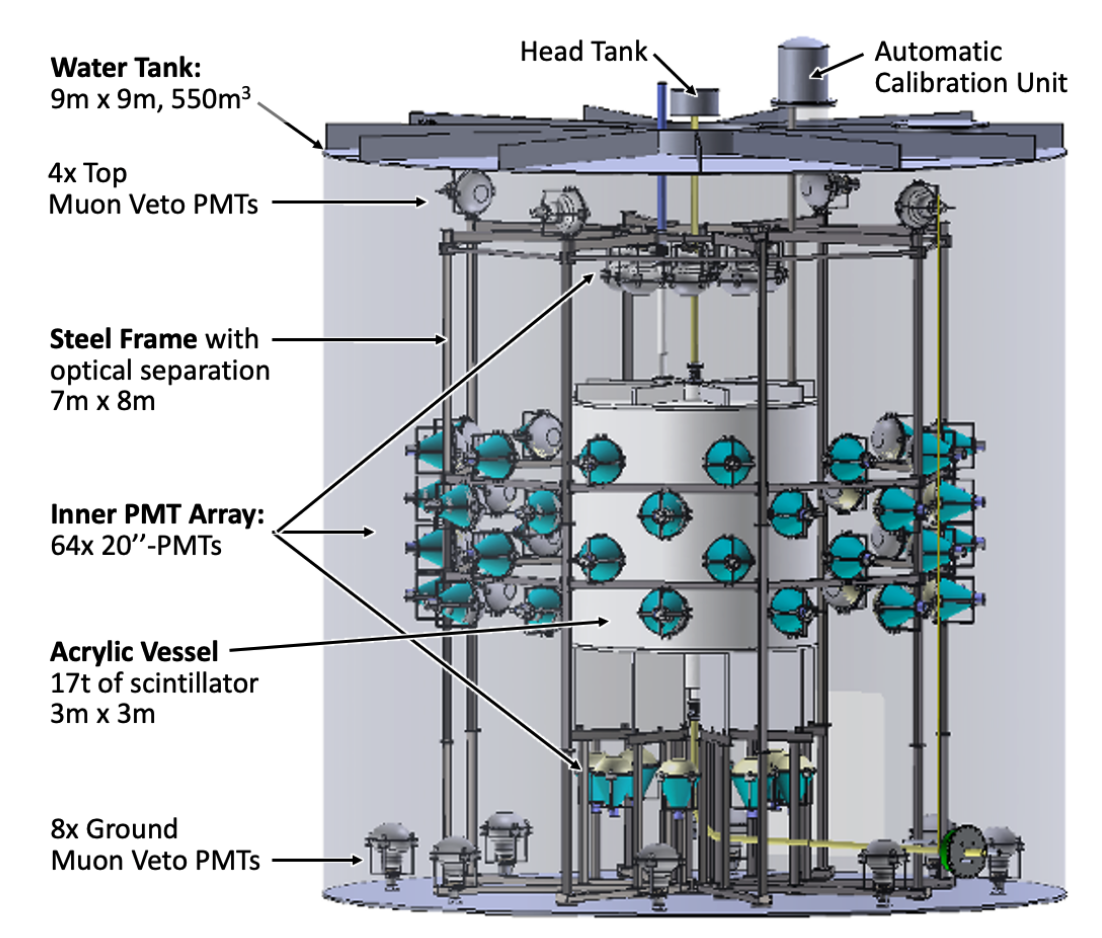
\includegraphics[width=\linewidth]{images/juno/osiris_schematic.png}
    \caption{Schematic of the OSIRIS satellite detector}
    \label{fig:juno:osiris}
  \end{subfigure}
  \caption{}
\end{figure}

\section{Software}
\label{sec:juno:software}

The simulation, reconstruction and analysis algorithms are all packaged in the JUNO software, subsequently called the software.
It is composed of multiple components integrated in the SNiPER \cite{lin_application_2017} framework:

\begin{itemize}
  \item Various primary particles simulators for the different kind of events, background and calibration sources.
  \item A Geant4 \cite{agostinelli_geant4simulation_2003, allison_geant4_2006, allison_recent_2016} Monte Carlo (MC) simulation containing the detectors geometries, a custom optical model for the LS and the supporting structures of the detectors. The Geant4 simulation integrate all relevant physics process for JUNO, validated by the collaboration. This step of the simulation is commonly called \textit{Detsim} and compute up to the production of photo-electrons in the PMTs. The optics properties of the different materials and detector components have been measured beforehand to be used to define the material and surfaces in the simulation.
  \item An electronic simulation, simulating the response waveform of the PMTs, tracking it through the digitization process, accounting for effects such as non-linearity, dark noise, Time Transit Spread (TTS), pre-pulsing, after-pulsing and ringing if the waveform. It's also the step handling the event triggers and mixing. This step is commonly referenced as \textit{Elecsim}.
  \item A waveform reconstruction where the digitized waveform are filtered to remove high-frequency white noise and then deconvoluted to yield time and charge informations of the photons hits on the PMTs. This step is commonly referenced as \textit{Calib}.
  \item The charge and time informations are used by reconstruction algorithms to reconstruct the interaction vertex and the deposited energy. This step is commonly reported as \textit{Reco}. See Section \ref{sec:juno:reco} for more details on the reconstruction.
  \item Once the singular events are reconstructed, they go through event pairing and classification to select IBD events. This step is named Event Classification.
  \item The purified signal is then analysed by the analysis framework which depend of the physics topic of interest. An introduction to the reactor $\bar{nu}_e$ is presented in Section \ref{sec:juno:Fit}.
\end{itemize}

The steps Reco and Event Classification are divided into two category of algorithm. Fast but less accurate algorithms that are running during the data taking designated as the \textit{Online} algorithms. Those algorithm are used to take the decision to save the event on tape or to throw it away. More accurate algorithms that run on batch of events designated \textit{Offline} algorithms. They are used for the physics analysis. The Offline Reco will be one of the main topic of interest for this thesis.


\section{Reactor anti-neutrino oscillation analysis}
\label{sec:juno:Fit}


\subsection{IBD samples selection}

The $\bar{\nu}_e$ coming from nuclear reactor will, for the most part, interact with proton, hydrogen nucleus, via Inverse Beta Decay (IBD).
The first step of the oscillation analysis is to constitute a sample of IBD candidates, dominated by actual IBDs. The IBD interaction, schematised in Figure \ref{fig:juno:IBD}, will produce two particle, with differentiable signals.

The first signal comes from the positron slowdown and its annihilation with an electron of the LS. This is the \textit{prompt} signal, happening a few ns after the IBD. The positron takes most of the $\bar{\nu}_e$ kinetic energy, as detailed in Section \ref{sec:juno:detct}.

The leftover kinetic energy is taken by the neutron that, after thermalisation in the LS, will be captured by an hydrogen and produce a 2.2 MeV gamma, or by a carbon emitting a 4.9 MeV gamma. This is the \textit{delayed} signal, happening $\sim$236 $\mu$s after the IBD. This second mono-energetic event serve as a marker for the IBD.

The IBD selection is thus based on the selection of a prompt event, with an energy between 0.8 and 12 MeV, and a delayed event with an energy in the ranges $[1.9, 2.5]$ MeV or $[4.4, 5.5]$ MeV. Those two signal needs to be in a 1 ms time window and within 1.5 m from each other. Additionally the two signal needs to be in a radius of 17.2m from the detector center (0.5 m from the edge) to protect from accidental background formed by two uncorrelated signals \cite{abusleme_potential_2024}. Those values will be further refined after once JUNO data-taking starts.

In addition, specials veto are setup to protect from cosmic muons and their aftermath. The details of those veto and selection can be found in \cite{abusleme_potential_2024}.

The expected rate and selection efficiency on IBD can be found in table \ref{tab:juno:ibd_selection}. After these selection, the residual background, including $\bar{\nu}_e$ coming from other sources than the reactor can be found in table \ref{tab:juno:res_bg}.

\begin{table}[ht]
  \centering
  \begin{tabular}{l|c|c}
    \hline
    Selection Criterion & Efficiency [\%] & IBD Rate [day$^{-1}$] \\
    \hline
    All IBDs            & 100.0           & 57.4 \\
    Fiducial Volume     & 91.5            & 52.5 \\
    IBD Selection       & 98.1            & 51.5 \\
    ~~Energy Range      & 99.8            & - \\
    ~~Time Correlation $(\Delta T_{p - d})$    & 99.0    & - \\
    ~~Spatial Correlation $(\Delta R_{p - d})$ & 99.2    & - \\
    Muon Veto (Temporal + Spatial)        & 91.6    & 47.1 \\
    \hline
    Combined Selection & 82.2             &47.1 \\
    \hline
  \end{tabular}
  \caption{Summary of cumulative reactor antineutrino selection efficiencies. The reported IBD rates (with baselines <300 km) refer to the expected events per day after the selection criteria are progressively applied. Table taken from \cite{abusleme_potential_2024}}
  \label{tab:juno:ibd_selection}
\end{table}

\begin{table}[ht]
  \centering
  \begin{tabular}{l|c|c}
    \hline
    Backgrounds           & Rate [day$^{-1}$] & B/S [\%] \\
    \hline
    Geoneutrinos          & 1.2               & 2.5 \\
    World reactors        & 1.0               & 2.1 \\
    Accidentals           & 0.8               & 1.7 \\
    $^9$Li/$^8$He         & 0.8               & 1.7 \\
    Atmospheric neutrinos & 0.16              & 0.34 \\
    Fast neutrons         & 0.1               & 0.21 \\
    $^{13}$C($\alpha$,n)$^{16}$O & 0.05       & 0.01 \\
    \hline
    Total backgrounds     & 4.11              & 8.7 \\
    \hline
  \end{tabular}
  \caption{Expected background rates, background to signal ratio (B/S), and rate and shape uncertainties. The B/S ratio is calculated by using the IBD signal rate of 47.1/day. Table taken from \cite{abusleme_potential_2024}}
  \label{tab:juno:res_bg}
\end{table}

Once a sample is obtained, the oscillation analysis will consist essentially on the fit of a spectrum model to the spectrum observed in the selected sample. More specifically, the spectrum under analysis is the spectrum of the reconstructed visible energy of the positron : $E^{vis}$.
The reconstruction is presented in detail in Section \ref{sec:juno:reco}. For 6 years of data taking, it will resemble that on Figure \ref{fig:juno:spectrum_with_background}. In the next sections, I describe the fit procedures developed in JUNO. This will be the occasion to introduce notions useful for Chapter \ref{sec:joint_fit}. Besides, I'll also describe the versions of the fit used in this Chapter \ref{sec:joint_fit}.

%- Ce qu'est le signal (une IBD)
%
%- Les grandes lignes de la selection (peut-être simplement dire que
%l'on s'appuie sur la coincidence en e+ et neutron)
%
%- Ce que sont les bruits de fond. J'imagine que tu n'as plus le temps
%de les décrire réellement. À inclure dans la "liste retard".
%
%- Une table donnant les yields de chacun pour une période donnée,
%à inclure en faisant écho à la figure 2.3

\subsection{Synthetic overview of fit procedures developed at JUNO}
\label{sec:juno:fit:subatech}

Several fit procedures are being developed by JUNO collaborators (half a dozen of groups work in parallel within the collaboration). We do not have the ambition of a thorough description here. Instead, we try to introduce the main elements useful to the reader to understand JUNO's future results, and the fit procedures used Chapter \ref{sec:joint_fit}.

In most cases, the fit is a binned fit to the histogrammed spectrum of $E_{vis}^{e^+}$, like the one in Figure \ref{fig:juno:spectrum_with_background}. It is is based on the minimization of a $\chi^2$ test statistics. Generically, it can be written this way :
\begin{equation}
  \label{eq:juno:chi2}
  \chi^2= \left(\bm{T}(\bm{\theta},\bm{\eta}) - \bm{D}  \right)^T V^{-1} \left(\bm{T}(\bm{\theta},\bm{\eta}) - \bm{D} \right) + \chi^2_{nuis}(\bm{\eta})
\end{equation}
where the components of data vector $\bm{D}$ are the number of events found in individual bins of the fitted histogram, $\bm{T}(\bm{\theta},\bm{\eta})$ is the vector of the predicted number of entries in each bins. This prediction is the integration over the width of the bins of the spectrum model for a given NMO (described latter in this section).

This model depends on the oscillation parameters $\bm{\theta} = \left(\Delta m^2_{21}, \sin^2(2\theta_{12}), \Delta m^2_{31}, \sin^2(2\theta_{13} )\right)$, and on nuisance parameters $\bm{\eta}$ involved in the fit model and associated with systematic uncertainties.
Uncertainties are treated in two ways : statistical and some of the systematic uncertainties are accounted for via the covariance matrix $V = V_{stat}+V_{syst}$; remaining systematic uncertainties are treated via the penalty term $\chi^2_{nuis}$, which is written this way :
\begin{equation}
  \label{eq:juno:nuis}
  \chi^2_{nuis}\left(\bm{\eta}\right)= \left(\bm{\eta}-\bm{\bar{\eta}}\right)^T \cdot V^{-1}_{\bm{\eta}}(\bm{\eta})  \cdot \left(\bm{\eta}-\bm{\bar{\eta}}\right)
\end{equation}
where $\bm{\bar{\eta}}$ is the vector containing the most probable values of the nuisance parameters according to our knowledge prior to the fit, and where $V_{\bm{\eta}}$ is the covariance matrix accounting of the uncertainty on these values, and the potential correlations between them.
In principles, a likelihood could be used instead of a $\chi^2$. However, some of the systematic uncertainties are not trivial to parameterize, therefore treating them as nuisance parameters in not trivial.

An example of nuisance parameters are the $A$, $B$ and $C$ parameters of equation \ref{eq:joint_fit:abc}, which can be used to describe the resolution on the reconstructed energy. The fit model leading to $\bm{T}\left(\bm{\theta},\bm{\eta}\right)$ indeed incorporates this resolution.

\subsubsection{Treatment of uncertainties}

Differences between various fit procedures developed within JUNO often lies in the choice of the systematic uncertainties that are treated via $V$ or $\chi^2_{nuis}(\bm{\eta})$. Among the reasons behind these differences is the necessity to compare several approaches to ensure the robustness JUNO's oscillation analysis results. This approach was already adopted in the recent evaluations of JUNO's potential \cite{abusleme_potential_2024, juno_collaboration_sub-percent_2022}. Studies carried out so far at Subatech assumes a treatment entirely via $V$.

Other differences lies in the choice of the way to evaluate $V_{stat}$. Two common approaches used in $\chi^2$ fit are the Neyman and the Pearson approaches. If the size of the fitted sample is high enough, the variation of $D_i$, the number of entries in bin $i$, around its true expectation value $\bar{D}_i$ is $\sqrt{\bar{D_i}}$. To evaluate this number, the Neyman approach uses simply the number of entries observed in the sample under analysis : $\sqrt{D_i}$. The Pearson approach uses the prediction by the fit model : $\sqrt{T(\bm{\theta},\bm{\eta})_i}$.

Both cases are approximations which lead to biases that are not tolerable given the precision JUNO must aim at for a successful oscillation analysis. To reduce this bias, most of JUNO groups employ the "Combined Neyman Pearson" approach introduced in \cite{ji_combined_2019}. Schematically, it consists on combining both approaches :
$\left(V_{stat}\right)_{ii} = 3/\left(\frac{1}{T(\bm{\theta},\bm{\eta})_i}+\frac{2}{D_i}\right)$.
Weights in this relation are chosen in order to cancel typical biases. The validity of this method is not guaranteed universally. In particular, limitations appear when a complex systematic matrix $V_{syst}$ is added to $V_{stat}$.

This is the case in the approach followed at Subatech, were all sources of systematic uncertainties are treated via this matrix. Dedicated studies run at Subatech observed biases in the fitted oscillation parameters using CNP in this case. Subatech's group therefore adopted another approach (verified to be unbiased).

Originally, fitting the $E^{e^+}_{vis}$ spectrum should mean maximising a likelihood, equal to the product over all bins of the probabilities to find $D_i$ in bin $i$. With a large enough samples, this product tends to a multidimensional gaussian (one dimension per bin) :
\begin{equation}
  \mathcal{L} = 2\pi^{-\frac{N}{2}} |V|^{-\frac{1}{2}}  e^{-\frac{1}{2}\left(\bm{D}-\bm{T}(\bm{\theta},\bm{\eta})\right)^T V^{-1} \left( \bm{D}-\bm{T}(\bm{\theta},\vec{\eta}) \right)}
\end{equation}
Replacing $\mathcal{L}$ by $-2 \ln \mathcal{L}$ one obtains :
\begin{equation}
\chi^2_{PV} = \left(\bm{T}(\bm{\theta},\bm{\eta}) - \bm{D} \right)^T V^{-1} \left(\bm{T}(\bm{\theta},\bm{\eta}) - \bm{D}  \right) + \ln(|V|)
\end{equation}
where $V$ is the total covariance matrix with its statistical component evaluated according to the Pearson approach. The $\ln|V|$ term, often neglected in $\chi^2$ fits, ensures that biases, essentially related to the normalisation of the fitted distribution, are avoided. This "PearsonV" $\chi^2$ is the one that we minimize in the fits used in Chapter \ref{sec:joint_fit}.

Another difference between the various procedures developed at JUNO is the choice of the spectrum range and binning. So far, at Subatech, we use an histogram defined between 0.8 and 9 MeV, and a regular binning involving 20 keV wide bins.

\subsubsection{Joint fit of JUNO and TAO spectra}

Another difference between the various fit procedures developed in the collaboration is the inclusion of the data collected by TAO (see Section \ref{sec:juno:tao}). The spectrum prediction $\bm{T}(\bm{\theta},\bm{\eta})$ involves predictions on the differential flux of $\bar{\nu}_e$ as a function of $E_{\bar{\nu}_e}$ produced in reactors. This is one of the main systematic uncertainties affecting the oscillation analysis. This can be constrained using the data of TAO. An efficient way to use them is via a simultaneous fit, which will constrain the part of the $\bm{\eta}$ parameters related to the reactor predictions. In this case, equation \ref{eq:juno:chi2} becomes :
\begin{equation}
  \chi^2 = \sum_{d}\left(\bm{T}^d(\bm{\theta}^d,\bm{\eta}) - \bm{D}^d  \right)^T V^{-1} \left(\bm{T}^d(\bm{\theta}^d,\bm{\eta}) - \bm{D}^d  \right) +  \chi^2_{nuis}(\bm{\eta})
\end{equation}
where the $d$ superscript stands for the spectrum measured in JUNO or TAO.

Finally, it must be noted that JUNO's sensitivity to $\sin^2(2\theta_{13})$ is too weak for a competitive measurement. In most versions of the oscillation analyses carried out within JUNO, it will be considered as a nuisance parameter. In practice, the various $\chi^2$'s presented earlier will receive an additional term :
\begin{equation}
  \chi^2_{\sin^2(2\theta_{13})} = \frac{(\sin^2(2\theta_{13})-\overline{\sin^2(2\theta_{13})})^2}{\sigma^2_{\overline{\sin^2(2\theta_{13})}}}
\end{equation}
where $\overline{\sin^2(2\theta_{13})}$ and the denominators can be provided, for instance, by the world average on this parameter.

\subsection{The spectrum model and sources of systematic uncertainties}

The $E^{e^+}_{vis}$ spectrum observed in data (Fig \ref{fig:juno:spectrum_with_background}) is the sum of the IBD spectrum and of the various backgrounds spectra (see table \ref{tab:juno:res_bg}).
The spectrum prediction $\bm{T}\left(\bm{\theta},\bm{\eta}\right)$ is therefore the sum of IBD and backgrounds predictions. The latter are provided by MC simulations. The former results from the theoretical description of the series of phenomena that lead to the observed IBD spectrum. In a given bin $i$, it can be expressed this way :
\begin{equation}
  \label{eq:juno:bin_content}
  T^i(\bm{\theta},\bm{\eta}) =\sum_{j} C_{ij}^{E_{rec}} \int_{E^{vis}_{j}}^{E^{vis}_{j+1}} \dd E^{vis} \int_{-1}^{1} \mathrm{dcos}\theta ~ \Phi(E^{\nu}) \frac{\dd\sigma}{\mathrm{dcos}\theta}(E^{\nu}, \cos\theta) \frac{\dd E^{\nu}}{\dd E^{dep}} \frac{\dd E^{dep}}{\dd E^{vis}}
\end{equation}
In the above equation, 4 kinds of energies appears: following the IBD, the antineutrino energy $E^{\nu}$ is quasi entirely transferred to the positron, of energy $E_{e}$. It eventually annihilates, so the actual energy released in the LS is $E_{dep}$, which includes the mass of the annihilated electron. The production optical photons is not linear in $E_{dep}$ (see Section \ref{sec:juno:calib}), so that the visible energy (that will be reconstructed) is $E_{vis}$. This reconstruction comes with resolution effects, leading to $E_{rec}$.

Equation \ref{eq:juno:bin_content} describe the passage from the original differential flux (as a function of $E^{\nu}$ ) of antineutrinos reaching the detector to the reconstructed spectrum:
\begin{itemize}
  \item $\Phi(E^{\nu})$ is the differential antineutrino flux reaching JUNO.
  \item $\frac{\dd\sigma}{\mathrm{dcos}\theta}(E^{\nu}, \cos\theta)$ account for the IBD cross section, which depends on the antineutrino energy and on the incidence angle.
  \item The last two terms of the integrand are the differential relations linking $E^{\nu}$, $E^{dep}$ and $E^{vis}$.
  \item Reconstruction effects are described via $C^{rec}_{ij}$'s, that make the link between the true and reconstructed visible energy. It a simple case, it is equivalent to a convolution product. The matrix formalism here prepares the fact that a realistic analysis might employ a more empirical way, based on MC.
\end{itemize}
\hfill

The differential flux is expressed this way:
\begin{equation}
\Phi(E^{\nu}) = \sum_{r} \left( \frac{{\cal P}_{\bar{\nu}_e\rightarrow \bar{\nu}_e}(E^{\nu},L_r)}{4\pi L^2_r} \frac{W_r}{\sum_{i} f_{i,r} e_i} \sum_{i} f_{i,r} s_i(E^{\nu}) \right)
\end{equation}
where:
\begin{itemize}
  \item ${\cal P}_{\bar{\nu}_e\rightarrow \bar{\nu}_e}(E^{\nu},L_r)$ is the antineutrino survival probability at distance $L_r$ from the production point in reactor $r$, dictated by the oscillation probability.
  \item $e_i$ stands for the mean energy released per fission for isotope $i$.
  \item $W_r$ is the thermal power of reactor $r$.
  \item $f_{i,r}$ is the fission fraction in reactor $r$ of isotope $i$ among the four.
  \item $s_i(E^{\nu})$ is the $\bar{\nu}_e$ energy spectrum - at emission point -  per fission for each isotope, as emitted by the reactor.
\end{itemize}
\hfill

\subsubsection{Sources of systematic uncertainties}

The numerous quantities appearing in the spectrum model embody a good part of the systematic uncertainties. Among the leading contributions are those related to the knowledge of the reactor related quantities. Of importance are also the uncertainties related to the modelling of the non linearity of the photon emission (passage from $E^{dep}$ to $E^{vis}$) and of the reconstruction resolution. The shape and rate of the backgrounds are also a leading source of systematic uncertainties. The uncertainty on IBD selection efficiency also has a notable role.

\subsubsection{Sensitivities to NMO and oscillation parameters}

JUNO will start taking data in 2025. During the months and years to come, oscillation analyses will naturally be optimized regularly. What we described here represent the state of the art mid 2024, and was used for the sensitivity studies published in \cite{abusleme_potential_2024, juno_collaboration_sub-percent_2022} and are presented in table \ref{tab:juno:juno-param-precision}

\begin{table}[ht]
  \centering
  \begin{small}
  \begin{tabular}{l | c c c c c}
    \hline
    & Central Value & PDG 2020 & 100 days & 6 years & 20 years \\
    \hline
    $\Delta m^2_{31} (\times 10^{-3} \mathrm{eV}^2)$ & 2.5283  & $\pm 0.034 ~ (1.3\%)$  & $\pm 0.021 ~ (0.8\%)$  & $\pm 0.0047 (0.2\%)$  & $\pm 0.0029 (0.1\%)$ \\
    $\Delta m^2_{21} (\times 10^{-3} \mathrm{eV}^2)$ & 7.53    & $\pm 0.18 ~ (2.4\%)$   & $\pm 0.074 ~ (1.0\%)$  & $\pm 0.024 (0.3\%)$   & $\pm 0.017  (0.2\%)$ \\
    $\sin ^2 \theta_{12}$                            & 0.307   & $\pm 0.013 ~ (4.2\%)$  & $\pm 0.0058 ~ (1.9\%)$ & $\pm 0.0016 (0.5\%)$  & $\pm 0.0010 (0.3\%)$ \\
    $\sin ^2 \theta_{13}$                            & 0.0218  & $\pm 0.0007 ~ (3.2\%)$ & $\pm 0.010 ~ (47.9\%)$ & $\pm 0.0026 (12.1\%)$ & $\pm 0.0016 (7.3\%)$ \\
    \hline
  \end{tabular}
\end{small}
  \caption{A summary of precision levels for the oscillation parameters. The reference value (PDG 2020 \cite{particle_data_group_review_2020}) is compared with 100 days, 6 years and 20 years of JUNO data taking.}
  \label{tab:juno:juno-param-precision}
\end{table}

\subsubsection{Asimov studies}
\label{sec:juno:Fit:asimov}

To study the behavior and performance of fit procedures with enough realism, one should perform fits to a large number of toy spectra, generated with a number events equal to what one expects in real data, for the given exposure under consideration. This allows to study the impact of realistic statistical fluctuations. This is, however, time consuming, since thousands of spectra have to be generated and fitted.

When subtle details are not crucial, another approach is possible to estimate sensitivities to the NMO and oscillation parameters, as well as (for instance) to verify the technical implementation of fitter (as we will do in Chapter \ref{sec:joint_fit} for the implementation of the joint fit). It consists on generating only 1 pseudo-data sample, where the content of each bin $D^i$ is set to the predicted value $T^i$, computed with a reasonable choice for the values of the model parameters (for instance, with the recent PDG values for the oscillation parameters). This is equivalent to a spectrum with fluctuations. It provides valid sensitivities if the expected statistics in the real data sample is high enough in each bin to assume a gaussian behavior.

\subsection{Versions of the fit used in this thesis}

In Chapter \ref{sec:joint_fit}, we'll study the potential of a particular application of Dual Calorimetry, call "Dual Calorimetry with neutrino oscillation." This approach require to perform fits to the $E^{vis}$ spectrum reconstructed with the LPMT system, with the SPMT system, and a joint fit to both spectra.

In the two former cases, the PearsonV $\chi^2$ introduced above will be used. In the latter case, it will be extended in the following way : The $\bm{D}$ data vector now possess 820 elements. Indeed, the fit is performed to a joint spectrum, where the LPMT spectrum is juxtaposed with the SPMT spectrum (see Figure \ref{fig:juno:joint_fit_spec}).

\begin{figure}[ht]
  \centering
  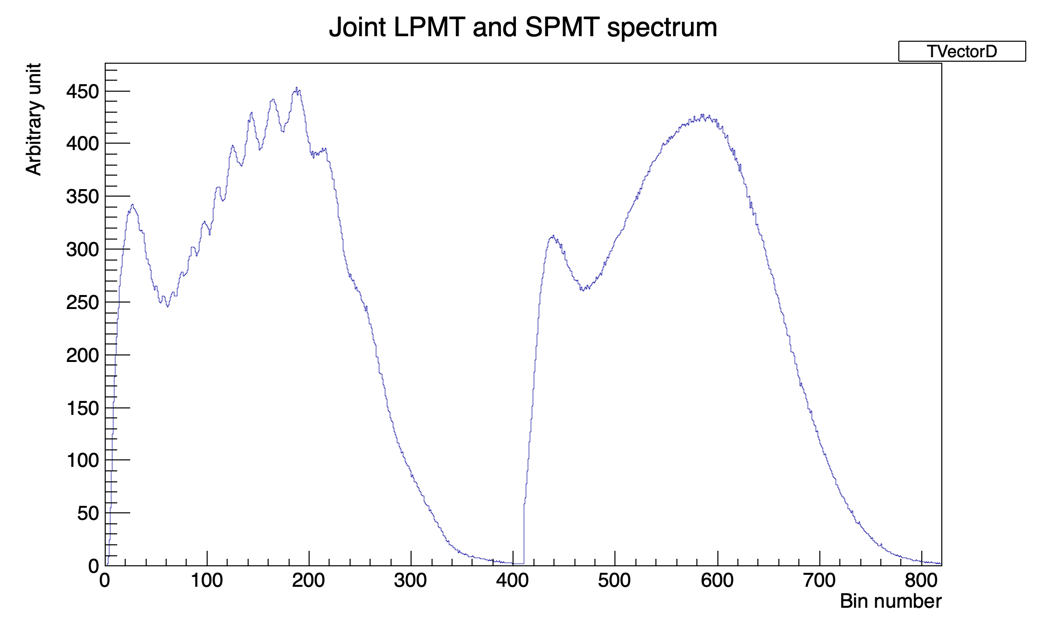
\includegraphics[height=5cm]{images/juno/joint_fit.png}
  \caption{Illustration of the spectrum considered when joint fitting}
  \label{fig:juno:joint_fit_spec}
\end{figure}

The prediction vector $\bm{T}\left(\bm{\theta}^d,\bm{\eta}\right)$ is naturally extended in the same way. Its components 1 to 410 predict the number of entries in the LPMT part of the LPMT+SPMT joint spectrum, while its components from 411 to 820 predict the contents of the SPMT part. Note that the list of oscillation parameters in $T_{411}(\bm{\theta}^d,\bm{\eta})$ to $T_{820}(\bm{\theta}^d,\bm{\eta})$ is the same as usual. However, $T_1(\bm{\theta}^d,\bm{\eta})$ to $T_{410}(\bm{\theta}^d,\bm{\eta})$ 2 additional parameters, $\delta \sin^2(2\theta_{12})$ and $\delta \Delta m^2_{21}$, are added to the corresponding oscillation parameters to account for a potential unexpected problem in the LPMT reconstruction or calibration.

In the case of this joint fit, the covariance matrix $V$ is extended to a $(820 \times 820)$ matrix. It is a central element of this study, as will be explained in Chapter \ref{sec:joint_fit}, since the LPMT and SPMT data spectrum are correlated, even at the statistical level. The determination of this matrix will be an important and original point.

Fits will be performed to an histogram spectrum defined over the 0.8-9 MeV range, with a flat binning (20 keV wide bins), often restricted to the 335 lowest $E^{vis}$ bins.

In this Section \ref{sec:juno:Fit}, we have provided a theoretical description of the fit procedures developed at JUNO. Software frameworks are necessary to use them in practice. The framework developed at Subatech will be described in Chapter \ref{sec:joint_fit}.


\section{State of the art of the Offline IBD reconstruction in JUNO}
\label{sec:juno:reco}

The main reconstruction method currently run in JUNO is a data-driven method based on a likelihood maximization \cite{wu_new_2019, huang_improving_2021} using only the LPMTs. The first step is to reconstruct the interaction vertex from which the energy reconstruction is dependent. It is also necessary for event pairing and classification.

\subsection{Interaction vertex reconstruction}

To start the likelihood maximization, a rough estimation of the vertex and of the event timing is needed. We start by estimating the vertex position using a charge based algorithm.

\subsubsection{Charge based algorithm}

The charge-based algorithm is basically base on the charge-weighted average of the PMT position.

\begin{align}
  \vec{r}_{cb} = a\cdot\frac{\sum_i q_i \cdot \vec{r}_i}{\sum_i q_i}
\end{align}

Where $q_i$ is the reconstructed charge of the pulse of the $i$th PMT and $\vec{r}_i$ is its position. $\vec{r}_0$ is the reconstructed interaction position. $a$ is a scale factor introduced because a weighted average over a 3D sphere is inherently biased. Using calibration we can estimate $a \approx 1.3$ \cite{li_event_2021}. The results in Figure \ref{fig:juno:rec:cbary} shows that the reconstruction is biased from around 15m and further. This is due to the phenomena called ``total reflection area'' or TR Area.

As depicted in the Figure \ref{fig:juno:rec:refl} the optical photons, given that they have a sufficiently large incidence angle, can be deviated of their trajectories when passing through the interfaces LS-acrylic and water-acrylic due to the optical index difference. This cause photons to be lost or to be detected by PMT further than anticipated if we consider their rectilinear trajectories. This cause the charge barycenter the be located closer to the center than the event really is.

\begin{figure}[ht]
  \begin{subfigure}[t]{0.48\textwidth}
    \centering
    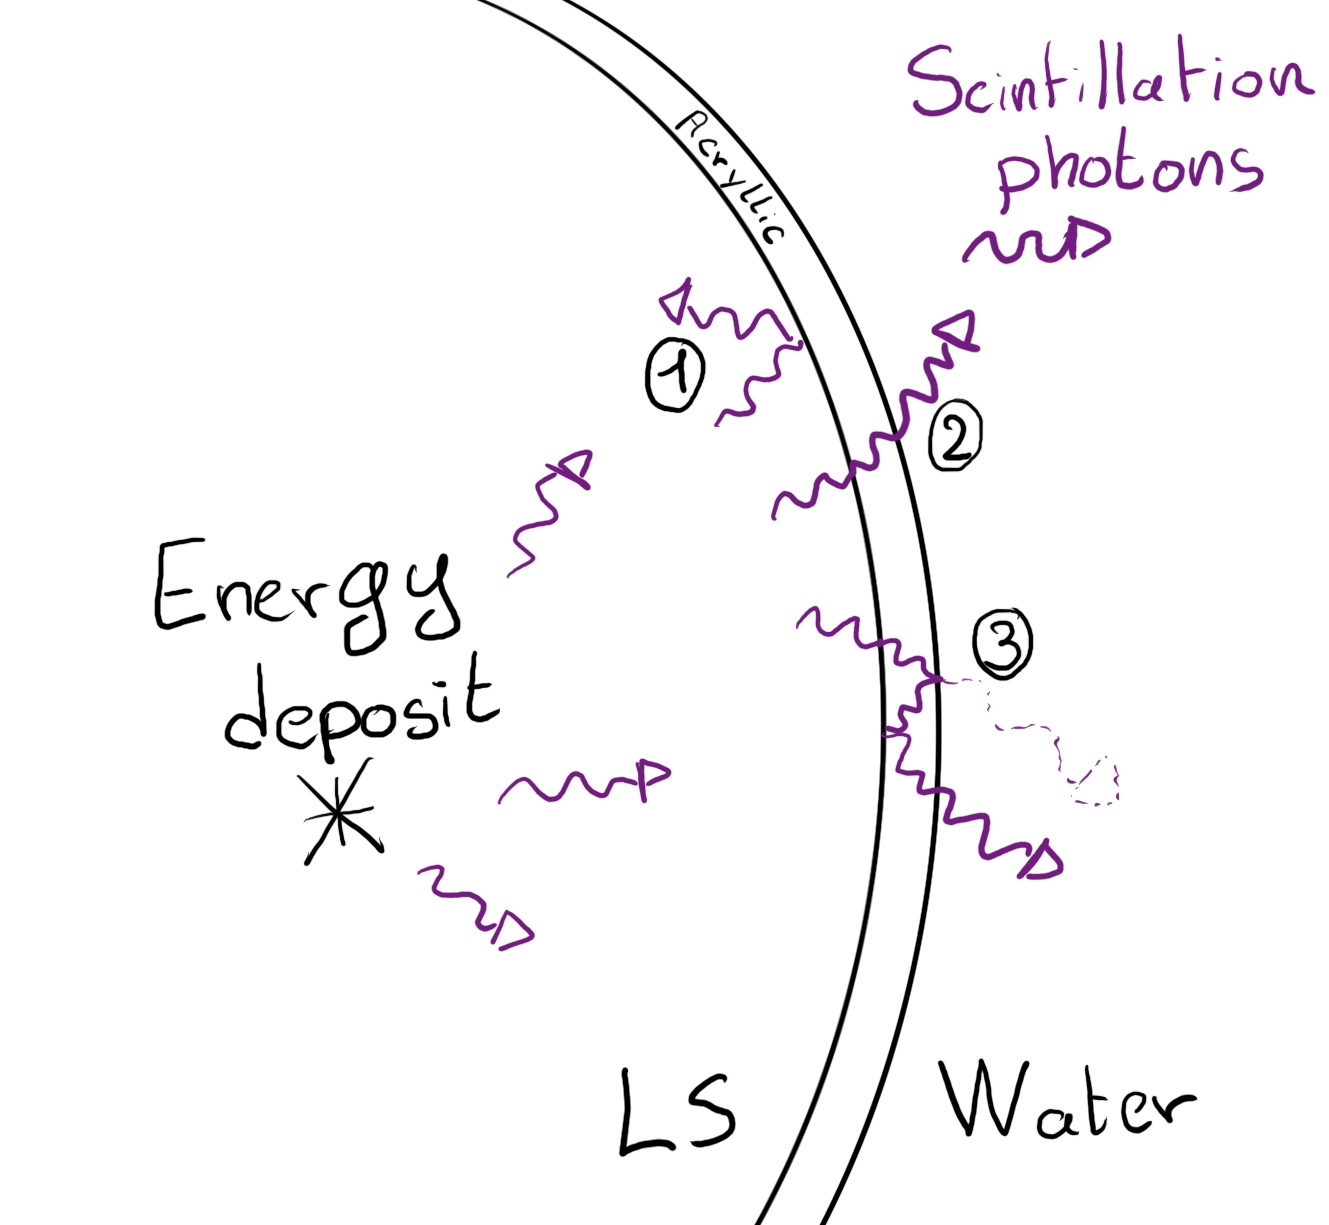
\includegraphics[height=6cm]{images/juno/reco/Reflexion_scenarii.jpg}
    \caption{Illustration of the different optical photons reflection scenarios. \textbf{1} is the reflection of the photon at the interface LS-acrylic or acrylic-water. \textbf{2} is the transmission of the photons through the interfaces. \textbf{3} is the conduction of the photon in the acrylic.}
    \label{fig:juno:rec:refl}
  \end{subfigure}
  \hfill
  \begin{subfigure}[t]{0.48\textwidth}
    \centering
    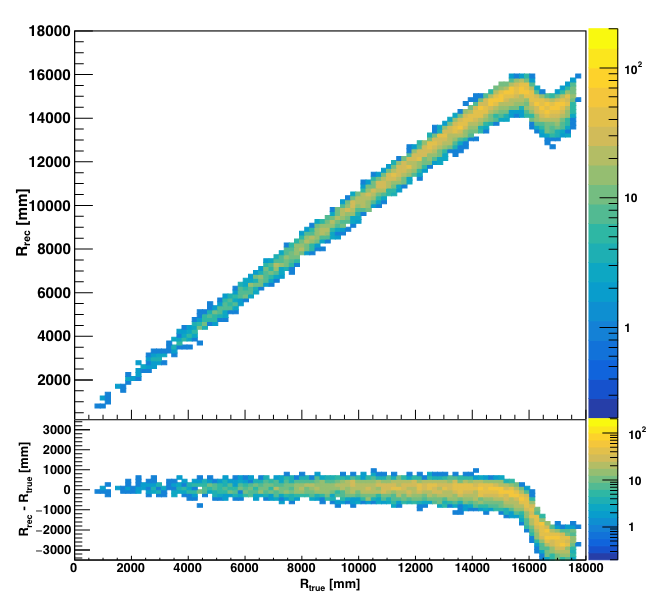
\includegraphics[height=6cm]{images/juno/reco/charge_barycenter.png}
    \caption{Heatmap of $R_{rec}$ and $R_{rec} - R_{true}$ as a function of $R_{true}$ for 4MeV prompt signals uniformly distributed in the detector calculated by the charge based algorithm}
    \label{fig:juno:rec:cbary}
  \end{subfigure}
  \caption{}
\end{figure}

It is to be noted that charge based algorithm, in addition to be biased near the edge of the detector, does not provide any information about the timing of the event. Therefore, a time based algorithm needs to be introduced to provide initial values.

\subsubsection{Time based algorithm}

The time based algorithm use the distribution of the time of flight corrections $\Delta t$ (Eq \ref{eq:juno:rec:tof_corr}) of an event to reconstruct its vertex and $t_0$. It follow the following iterations:

\begin{enumerate}
  \item Use the charge based algorithm to get an initial vertex to start the iteration.

  \item \label{alg:rec:tba} Calculate the time of flight correction for the $i$th PMT using \begin{equation}
      \label{eq:juno:rec:tof_corr}
      \Delta t_i (j) = t_i - \mathrm{tof}_i (j)
    \end{equation}
    where $j$ is the iteration step, $t_i$ is the timing of the $i$th PMT, and $\mathrm{tof}_i$ is the time-of-flight of the photon considering an rectilinear trajectory and an effective velocity in the LS and water (see \cite{li_event_2021} for detailed description of this effective velocity). Plot the $\Delta t$ distribution and label the peak position as $\Delta t^{\mathrm{peak}}$ (see fig \ref{fig:juno:rec:delta_t_distrib}).

  \item Calculate a correction vector $\vec{\delta} [\vec{r}(j)]$ as \begin{equation}
      \vec{\delta} [\vec{r}(j)] = \frac{\sum_i \bigg(\frac{\Delta t(j) - \Delta t^{\mathrm{peak}}(j)}{\mathrm{tof}_i(j)} \bigg) \cdot (\vec{r}_0(j) - \vec{r}_i)}{N^{\mathrm{peak}}(j)}
    \end{equation}
    where $\vec{r}_0$ is the vertex position at the beginning of this iteration, $\vec{r}_i$ is the position of the $i$th PMT. To minimize the effect of scattering, dark noise and reflection, only the pulse happening in a time window (-10 ns, +5 ns) around $\Delta t^{\mathrm{peak}}$ are considered. $N^{\mathrm{peak}}$ is the number of PE collected in this time-window.

  \item if $\vec{\delta} [\vec{r}(j)] < 1 \mathrm{mm}$ or $j \geq 100$, stop the iteration. Otherwise $\vec{r}_0 (j + 1) = \vec{r}_0 (j) + \vec{\delta} [\vec{r}(j)]$ and go to step \ref{alg:rec:tba}.
\end{enumerate}

\begin{figure}
  \begin{subfigure}[t]{0.48\textwidth}
    \centering
    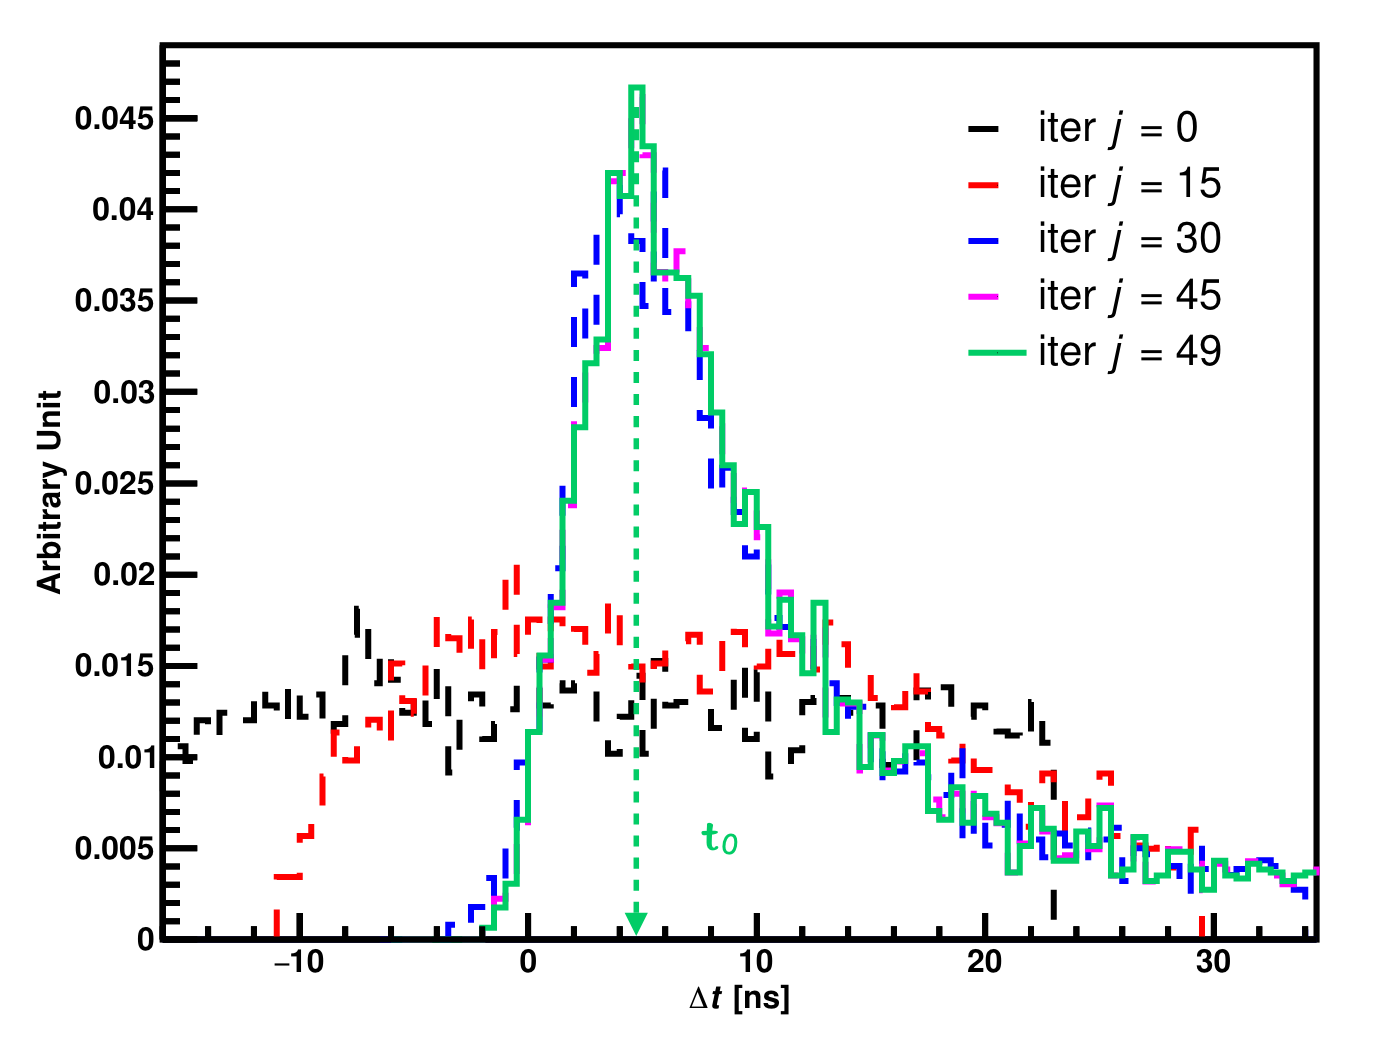
\includegraphics[width=\textwidth]{images/juno/reco/delta_t_peak_distrib.png}
    \caption{$\Delta t$ distribution at different iterations step $j$}
    \label{fig:juno:rec:delta_t_distrib}
  \end{subfigure}
  \hfill
  \begin{subfigure}[t]{0.48\textwidth}
    \centering
    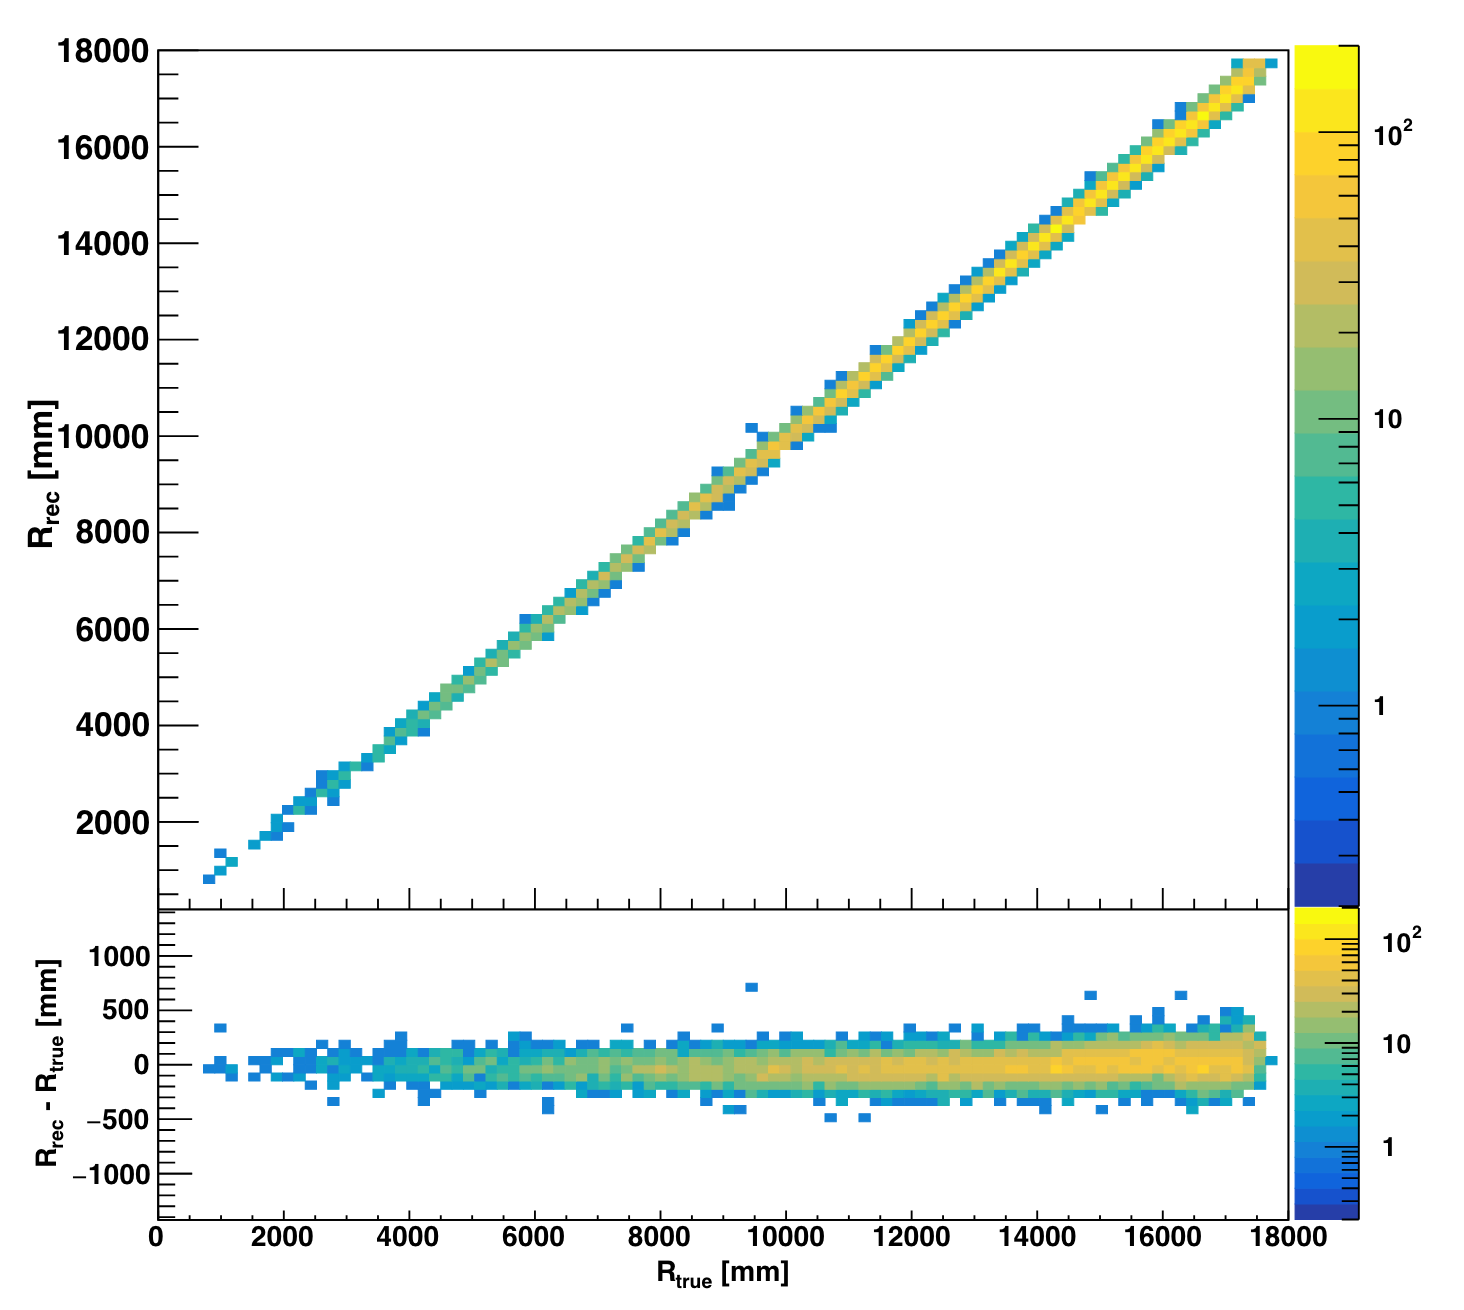
\includegraphics[width=\textwidth]{images/juno/reco/time_based_algorithm.png}
    \caption{Heatmap of $R_{rec}$ and $R_{rec} - R_{true}$ as a function of $R_{true}$ for 4MeV prompt signals uniformly distributed in the detector calculated by the time based algorithm}
    \label{fig:juno:rec:time_based_results}
  \end{subfigure}
  \caption{}
\end{figure}

However because the earliest arrival time is used, $t_i$ is related to the number photoelectrons $N_i^{\mathrm{pe}}$ detected by the PMT \cite{ranucci_analytical_1995, galbiati_time_2006, moszynski_status_1979}. To reduce bias in the vertex reconstruction, the following equation is used to correct $t_i$ into $t'_i$:
\begin{equation}
  t'_{i} = t_i - p_0 / \sqrt{N_i^{\mathrm{pe}}} - p_1 - p_2 / N_i^{\mathrm{pe}}
\end{equation}

The parameters $(p_0, p_1, p_2)$ were optimized to (9.42, 0.74, -4.60) for Hamamatsu PMTs and (41.31, -12.04, -20.02) for NNVT PMTs \cite{li_event_2021}. The results presented in Figure \ref{fig:juno:rec:time_based_results} shows that the time based algorithm provide a more accurate vertex and is unbiased even in the TR area. This results $(\vec{r}_0, t_0)$ is used as initial value for the likelihood algorithm.

\subsubsection{Time likelihood algorithm}

The time likelihood algorithm use the residual time expressed as follow
\begin{equation}
  \label{eq:juno:rec:t_res}
  t_{\mathrm{res}}^i(\vec{r}_0, t_0) = t_i - \mathrm{tof}_i - t_0
\end{equation}

In a first order approximation, the scintillator time response Probability Density Function (PDF) can be described as the emission time profile of the scintillation photons, the Time Transit Spread (TTS) and the dark noise of the PMTs. The emission time profile $f(t_{\mathrm{res}})$ is described like
\begin{equation}
  f(t_{\mathrm{res}}) = \sum_k \frac{\rho_k}{\tau_k} e^{\frac{-t_{\mathrm{res}}}{\tau_k}}, ~ \sum_k \rho_k = 1
\end{equation}
as the sum of the $k$ component that emit light in the LS each one characterised by it's decay time $\tau_k$ and intensity fraction $\rho_k$. The TTS component is expressed as a gaussian convolution
\begin{equation}
  g(t_{\mathrm{res}}) = \frac{1}{\sqrt{2\pi}\sigma}e^{\frac{-(t_{\mathrm{res}} - \nu)^2}{2\sigma^2}} \cdot f(t_{\mathrm{res}})
\end{equation}
where $\sigma$ is the TTS of PMTs and $\nu$ is the average transit time. The dark noise is not correlated with any physical events and considered as constant rate over the time window considered $T$. By normalizing the dark noise probability $\epsilon(t_{\mathrm{res}})$ as $\int_T \epsilon(t_{\mathrm{res}}) dt_{\mathrm{res}} = \epsilon_{\mathrm{dn}}$ , it can be integrated in the PDF as
\begin{equation}
  \label{eq:juno:juno:tim_like:dn}
  p(t_{\mathrm{res}}) = (1-\epsilon_{\mathrm{dn}}) \cdot g(t_{\mathrm{res}}) + \epsilon(t_{\mathrm{res}})
\end{equation}

The distribution of the residual time $t_{\mathrm{res}}$ of an event can then be compared to $p(t_{\mathrm{res}})$ and the best fitting vertex $\vec{r}_0$ and $t_0$ can be chosen by minimizing
\begin{equation}
  \mathcal{L}(\vec{r}_0, t_0) = - \mathrm{ln} \bigg(\prod_i p(t^i_{\mathrm{res}}) \bigg)
\end{equation}

The parameter of Eq. \ref{eq:juno:juno:tim_like:dn} can be measured experimentally. The results shown in Figure \ref{fig:juno:rec:time_likelihood} used PDF from monte carlo simulation. The results shows that $R_{rec} - R_{true}$ is biased depending on the energy. While this could be corrected using calibration, another algorithm based on charge likelihood was developed to correct this problem.

\begin{figure}[ht]
  \centering
  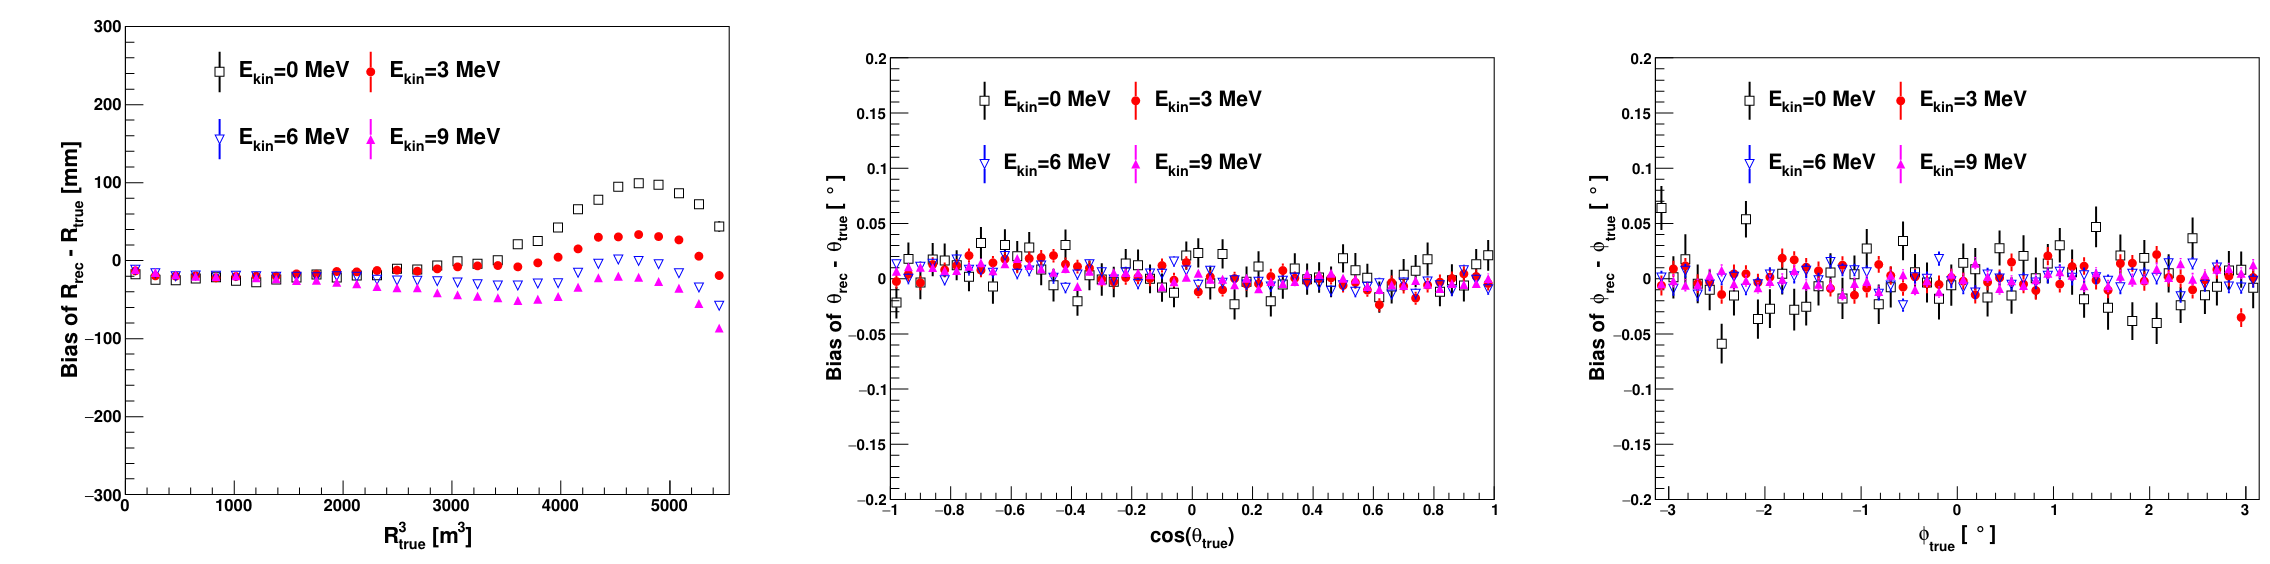
\includegraphics[width=\linewidth]{images/juno/reco/time_likelihood_results.png}
  \caption{Bias of the reconstructed radius R (left), $\theta$ (middle) and $\phi$ (right) for multiple energies by the time likelihood algorithm}
  \label{fig:juno:rec:time_likelihood}
\end{figure}


\subsubsection{Charge likelihood algorithm}

Similarly to the time likelihood algorithms that use a timing PDF, the charge likelihood algorithm use a PE PDF for each PMT depending on the energy and position of the event. With $\mu(\vec{r}_0, E)$ the mean expected number of PE detected by each PMT, the probability to observe $N_{pe}$ in a PMT follow a Poisson distribution. Thus
\begin{itemize}
  \item The probability to observe no hit ($N_{pe} = 0$) in the $j$th PMT is $P^{j}_{nohit} (\vec{r}_0, E) = e^{-\mu_j}$
  \item The probability to observe $N_{pe} \neq 0$ in the $i$th PMT is $P^{i}_{hit} (\vec{r}_0, E) = \frac{\mu^{N^i_{pe}} e^{-\mu_i}}{N^i_{pe}!}$
\end{itemize}

Therefore, the probability to observe a specific hit pattern can be expressed as
\begin{equation}
  P(\vec{r}_0, E) = \prod_j P^j_{nohit}(\vec{r}_0, E) \cdot \prod_i P^i_{hit}(\vec{r}_0, E)
\end{equation}

The best fit values of $\vec{R}_0$ and $E$ can then be calculated by minimizing the negative log-likelihood
\begin{equation}
  \label{eq:juno:rec:charge_likelihood}
  \mathcal{L}(\vec{r}_0, E) = - \mathrm{ln}(P(\vec{r}_0,E))
\end{equation}

In principle, $\mu_i(\vec{r}_0, E)$ could be expressed
\begin{equation}
  \label{eq:juno:rec:mu_i}
  \mu_i(\vec{r}_0, E) = Y \cdot \frac{\Omega(\vec{r}_0, r_i)}{4 \pi} \cdot \epsilon_i \cdot f(\theta_i) \cdot e^{-\sum_m \frac{d_m}{\zeta_m}}\cdot E + \delta_i
\end{equation}
where $Y$ is the energy scale factor, $\Omega(\vec{r}_0, r_i)$ is the solid angle of the $i$th PMT, $\epsilon_i$ is its detection efficiency, $f(\theta_i)$ its angular response, $\zeta_m$ is the attenuation length in the materials and $\delta_i$ the expected number of dark noise.

However Eq. \ref{eq:juno:rec:mu_i} assume that the scintillation light yield is linear with energy and describe poorly the contribution of indirect light, shadow effect due to the supporting structure and the total reflection effects. The solution is to use data driven methods to produce the pdf by using the calibrations sources and position described in Section \ref{sec:juno:calib}. In the results presented in Figures \ref{fig:juno:rec:time_charge_results}, the PDF was produced using MC simulation and 29 specific calibrations position \cite{li_event_2021} along the Z-axis of the detector.
\begin{figure}[ht]
  \centering
  \begin{subfigure}[b]{0.48\linewidth}
    \centering
    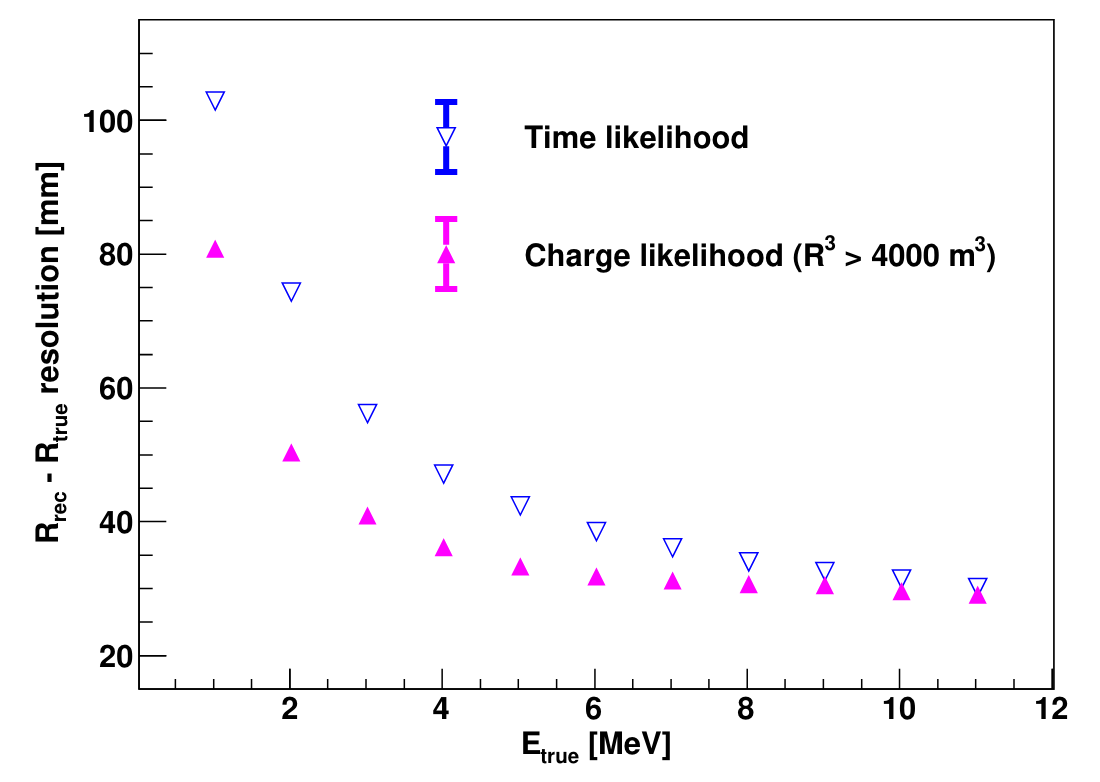
\includegraphics[width=\textwidth]{images/juno/reco/charge_likelihood_res.png}
  \end{subfigure}
  \hfill
  \begin{subfigure}[b]{0.48\linewidth}
    \centering
    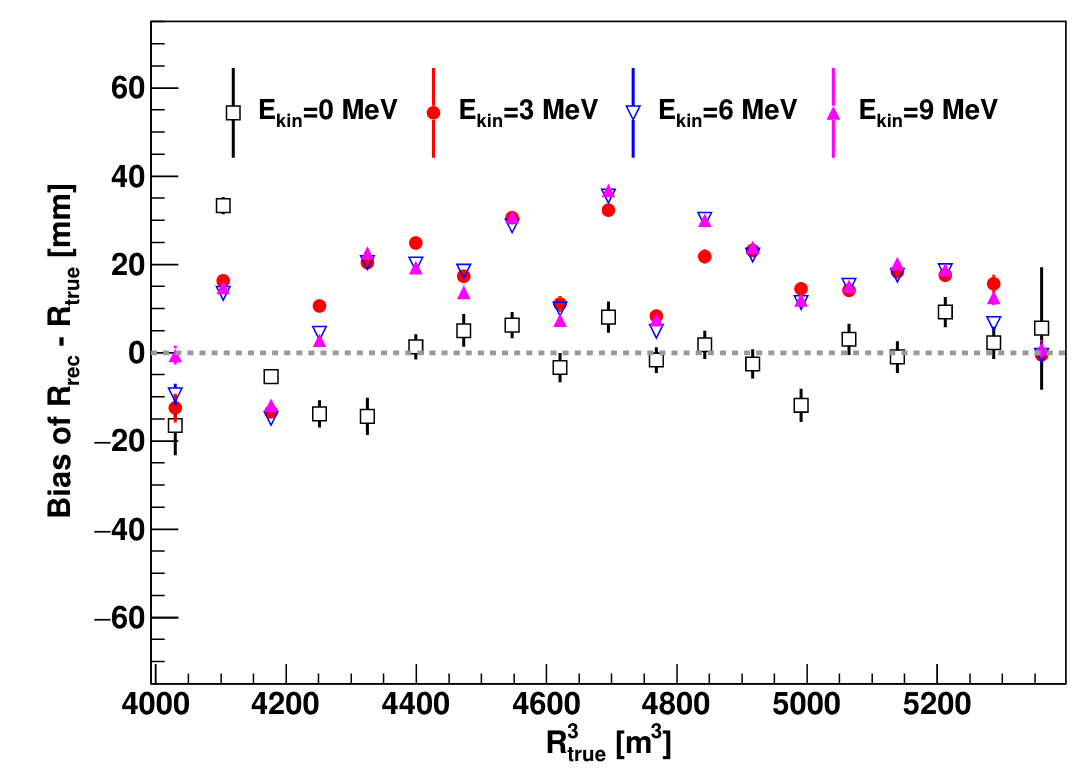
\includegraphics[width=\textwidth]{images/juno/reco/charge_likelihood_bias.png}
  \end{subfigure}
  \caption{\textbf{On the left:} Resolution of the reconstructed R as a function of the energy in the TR area ($R^3 > 4000 \mathrm{m}^3 \equiv R > 16 m$) by the charge and time likelihood algorithms. \textbf{On the right:} Bias of the reconstructed R in the TR area for different energies by the charge likelihood algorithm}
  \label{fig:juno:rec:time_charge_results}
\end{figure}
We see that the charge likelihood algorithm show little bias in the TR area and a better resolution than the time likelihood. The Figure \ref{fig:juno:rec:all_class} shows the radial resolution of the different algorithm presented for this section, we can see the refinement at each step and that the charge likelihood yield the best results.

\begin{figure}[ht]
  \centering
  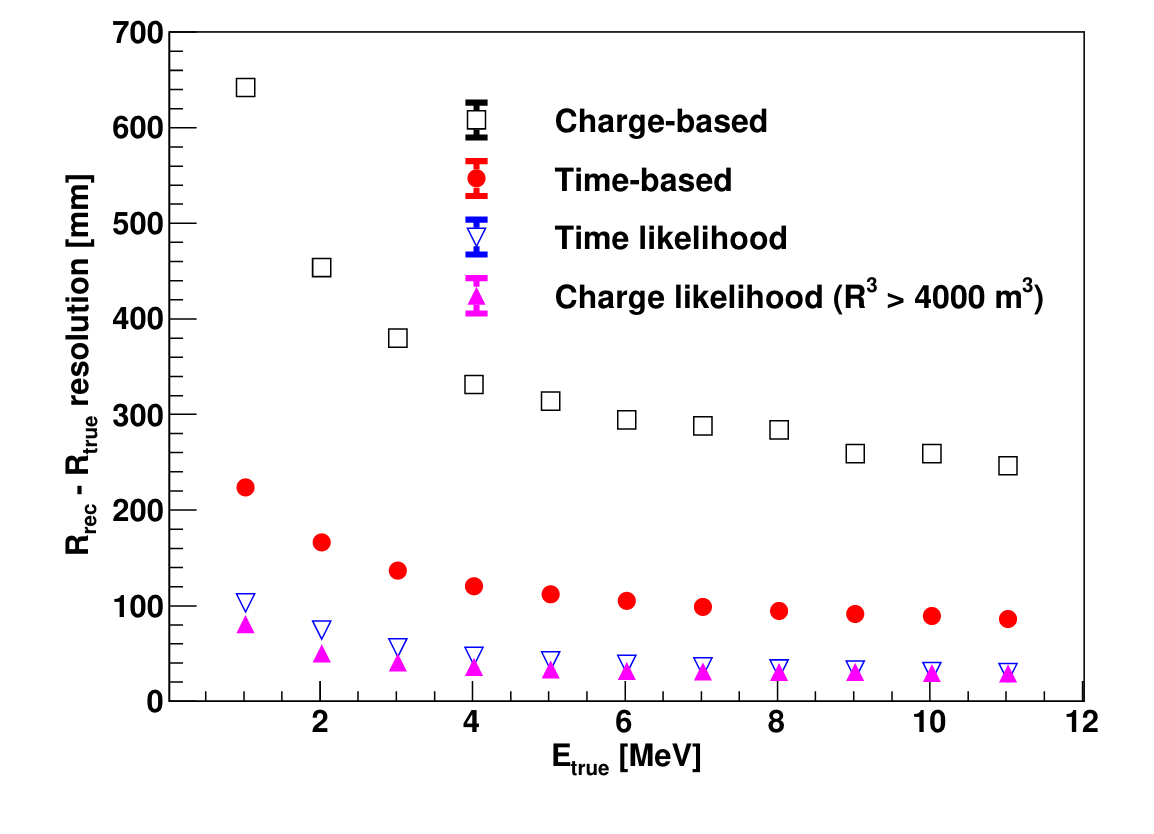
\includegraphics[height=6cm]{images/juno/reco/vertex_reco_classique.png}
  \caption{Radial resolution of the different vertex reconstruction algorithms as a function of the energy}
  \label{fig:juno:rec:all_class}
\end{figure}

The charge based likelihood algorithms already give use some information on the energy as Eq. \ref{eq:juno:rec:charge_likelihood} is minimized but the energy can be further refined as shown in the next section.


\subsection{Energy reconstruction}

As explained in Section \ref{sec:juno:nom_precise_measurement}, energy resolution is crucial for the NMO and oscillation parameters measurements. Thus the energy reconstruction algorithm should take into consideration as much detector effect as possible. The following method is a data driven method based on calibration samples inspired by the charge likelihood algorithm described above \cite{huang_data-driven_2023}.


\begin{figure}[ht]
  \begin{subfigure}[b]{0.48\linewidth}
    \centering
    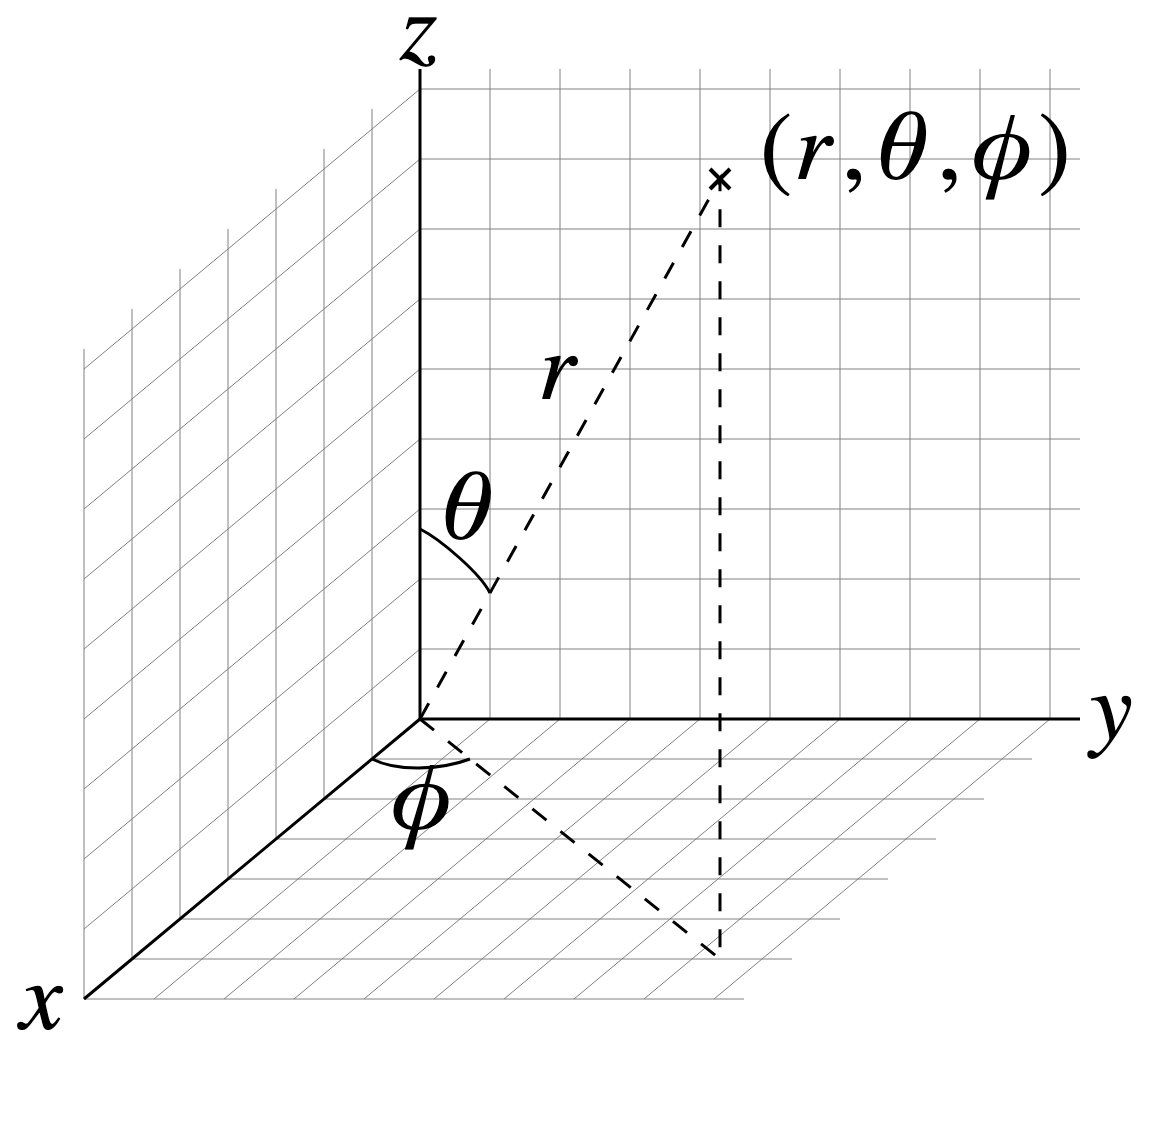
\includegraphics[height=6cm]{images/juno/spherical_coordinate_system.png}
    \caption{Spherical coordinate system used in JUNO for reconstruction}
    \label{fig:juno:rec:corrdinate_system}
  \end{subfigure}
  \hfill
  \begin{subfigure}[b]{0.48\linewidth}
    \centering
    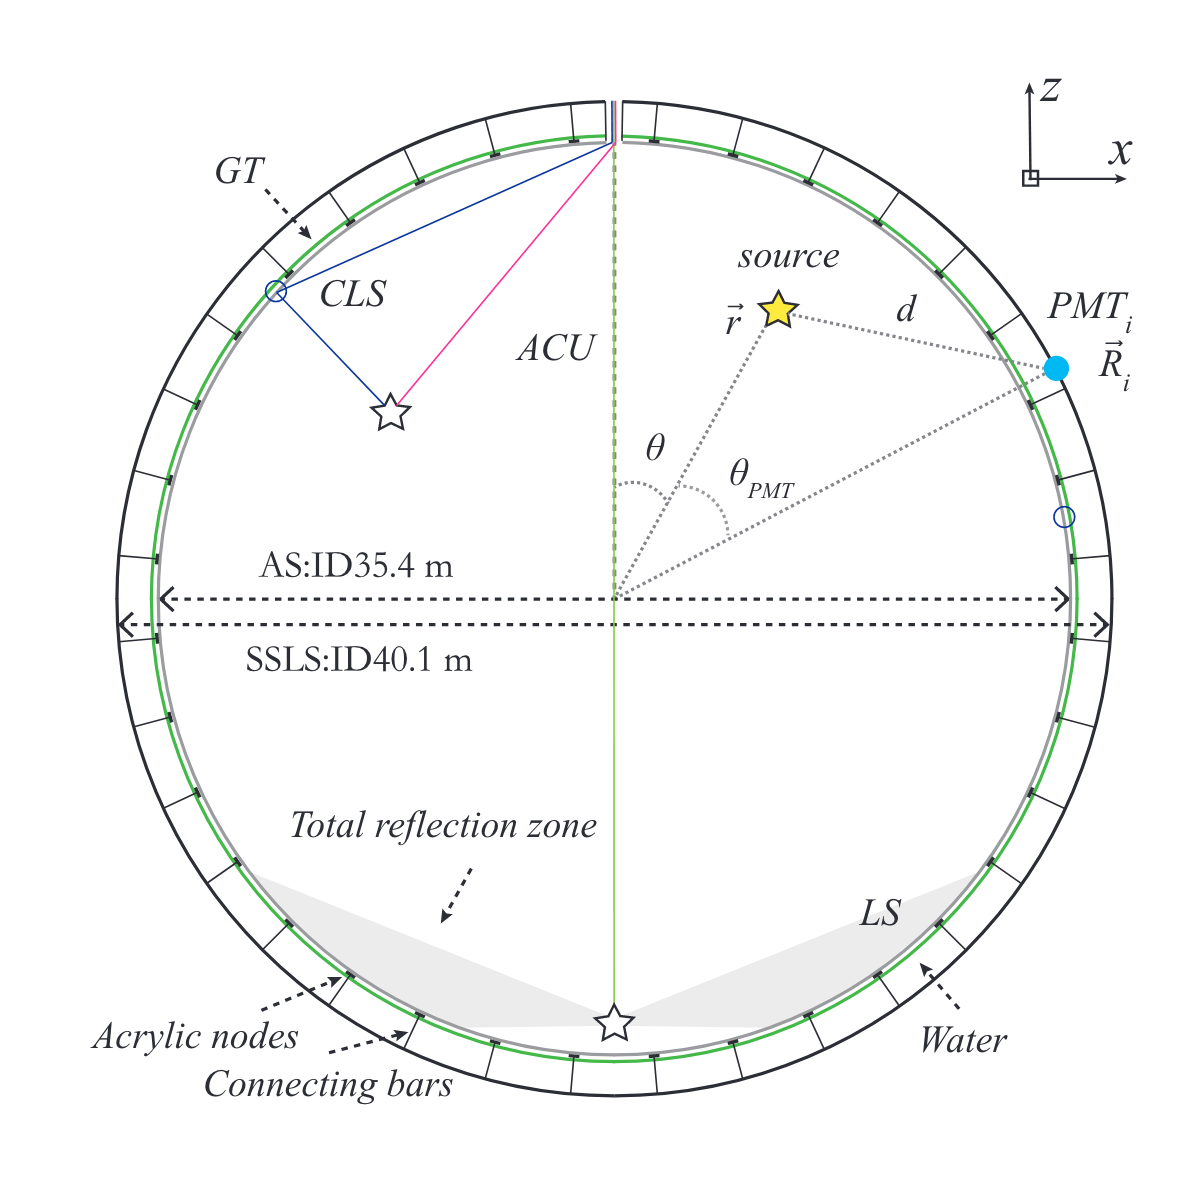
\includegraphics[height=6cm]{images/juno/reco/energy_reco_vars.png}
    \caption{Definition of the variables used in the energy reconstruction}
    \label{fig:juno:rec:energy_vars}
  \end{subfigure}
  \caption{}
\end{figure}

\subsubsection{Charge estimation}

The most important element in the energy reconstruction is $\mu_i(\vec{r}_0, E)$ described in Eq. \ref{eq:juno:rec:mu_i}. For realistic cases, we also need to take into account the electronics effect that were omitted in the previous section. Those effect will cause a charge smearing due to the uncertainties in the $N_{pe}$ reconstruction. Thus we define $\hat{\mu}^L(\vec{r}_0, E)$ which is the expected $N_{pe}/E$ in the whole detector for an event with visible energy $E_{vis}$ and position $\vec{r}_0$. The position of the event and PMTs are now defined using $(r, \theta, \theta_{pmt})$ as defined in Figure \ref{fig:juno:rec:energy_vars}.
\begin{equation}
  \label{eq:juno:reco:charge_est}
  \hat{\mu}(r, \theta, \theta_{pmt}, E_{vis}) = \frac{1}{E_{vis}} \frac{1}{M} \sum_i^M\frac{\frac{\bar{q}_i}{\hat{Q}_i} - \mu_i^D}{\mathrm{DE}_i}, ~ \mu_i^D = \mathrm{DNR}_i \cdot L
\end{equation}
where $i$ runs over the PMTs with the same $\theta_{pmt}$, $\mathrm{DE}_i$ is the detection efficiency of the $i$th PMT. $\mu_i^D$ is the expected number of dark noise photoelectrons in the time window $L$. The time window have been optimized to $L = 280 ~ \mathrm{ns}$ \cite{huang_data-driven_2023}. $\bar{q}_i$ is the average recorded photoelectrons in the time window and $\hat{Q}_i$ is the expected average charge for 1 photoelectron. The $N_{pe}$ map is constructed following the procedure described in \cite{huang_improving_2021}.

\subsubsection{Time estimation}

The second important observable is the hit time of photons that was previously defined in Eq. \ref{eq:juno:rec:t_res}. It is here refined as
\begin{equation}
  t_r = t_h - \mathrm{tof} - t_0 = t_{LS} + t_{TT}
\end{equation}
where $t_h$ is the time of hit, $t_{LS}$ is the scintillation time and $t_{TT}$ the transit time of PMTs that is described by a gaussian
\begin{equation}
  t_{TT} = \mathcal{N}(\overline{\mu_{TT} + t_{d}}, \sigma_{TT})
\end{equation}
where $\mu_{TT}$ is the mean transit time in PMTs, $\sigma_{TT}$ is the Transit Time Spread (TTS) of the PMTs and $t_{d}$ is the delay time in the electronics. The effective refraction index of the LS is also corrected to take into account the propagation distance in the detector.

The timing PDF $P_T(t_r | r,d,\mu_l,\mu_d,k)$ can now be generated using calibration sources \cite{huang_data-driven_2023}. This PDF describe the probability that the residual time of the first photon hit is in $[t_r, t_r + \delta]$ with $r$ the radius of the event vertex, $d = |\vec{r} - \vec{r}_{PMT}|$ the propagation distance, $\mu_l$ and $\mu_d$ the expected number of PE and dark noise in the electronic reading window and $k$ is the detected number of PE.

Now let denote $f(t, r, d)$ the probability density function of "photoelectron hit a time t" for an event happening at $r$ where the photons traveled the distance $d$ in the LS
\begin{equation}
  F(t, r, d) = \int_t^L f(t', r, d)dt'
\end{equation}
Based on the PDF for one photon $k=1$, one can define
\begin{equation}
  P^l_T(t|k=n) = I^l_n [f_l(t)F^{n-1}_l(t)]
\end{equation}
where the indicator $l$ means that the photons comes from the LS and $I^l_n$ a normalisation factor. To this pdf we add the probability to have photons coming from the dark noise indicated by the indicator $d$ using
\begin{equation}
  f_d(t) = 1 / L, ~ F_d(t) = 1 - \frac{t}{L}
\end{equation}
and so for the case where only one photon is detected by the PMT ($k=1$)
\begin{equation}
  P_T(t|\mu_l, \mu_d, k = 1) = I_1 [ P(1, \mu_l) P(0, \mu_d) f_l(t) + P(0, \mu_l) P(1, \mu_d) f_d(t) ]
\end{equation}
where $P(k_\alpha, \mu_\alpha)$ is the Poisson probability to detect $k_\alpha$ PE from $\alpha \in \{l, d\}$ with the condition $k_l + k_d = k$.

Now that we have the individual timing and charge probability we can construct the charge likelihood referred as QMLE:
\begin{equation}
  \mathcal{L}(q_1, q_2, ..., q_N | \vec{r}, E_{vis}) = \prod_{j \in \mathrm{unfired}} e^{-\mu_j} \prod_{i \in \mathrm{fired}} \bigg(\sum_{k=1} P_Q(q_i|k) \cdot P(k, \mu_i) \bigg)
\end{equation}
where $\mu_i = E_{vis} \hat{\mu_i^L} + \mu_i^D$ and $P(k, \mu_i)$ is the Poisson probability of observing k PE. $P_Q(q_i|k)$ is the charge pdf for $k$ PE. And we can also construct the time likelihood referred as TMLE:
\begin{equation}
  \mathcal{L}(t_{1,r}, t_{2,r}, ..., t_{N,r} | \vec{r}, t_0) = \prod_{i \in \mathrm{hit}} \frac{\sum_{k=1}^K P_T(t_{i,r} | r, d, \mu_i^l, \mu_i^d, k) \cdot P(k, \mu^l_i + \mu^d_i)}{\sum_{k=1}^K P(k, \mu^l_i + \mu^d_i)}
\end{equation}
where $K$ is cut to 20 PE and hit is the set of hits satisfying $-100 < t_{i,r} < 500$ ns.

Merging those two likelihood give the charge-time likelihood QTMLE
\begin{equation}
  \mathcal{L}(q_1, q_2, ..., q_N; t_{1,r}, t_{2,r}, ..., t_{N,r} | \vec{r}, t_0 , E_{vis}) = \mathcal{L}(q_1, q_2, ..., q_N | \vec{r}, E_{vis}) \cdot \mathcal{L}(t_{1,r}, t_{2,r}, ..., t_{N,r} | \vec{r}, t_0)
\end{equation}

The radial and energy resolutions of the different likelihood are presented in Figure \ref{fig:juno:rec:qtmle} (from \cite{huang_data-driven_2023}). We can see the improvement of adding the time information to the vertex reconstruction and that an increase in vertex precision can bring improvement in the energy resolution, especially at low energies.

\begin{figure}[ht]
  \begin{subfigure}{0.48\linewidth}
    \centering
    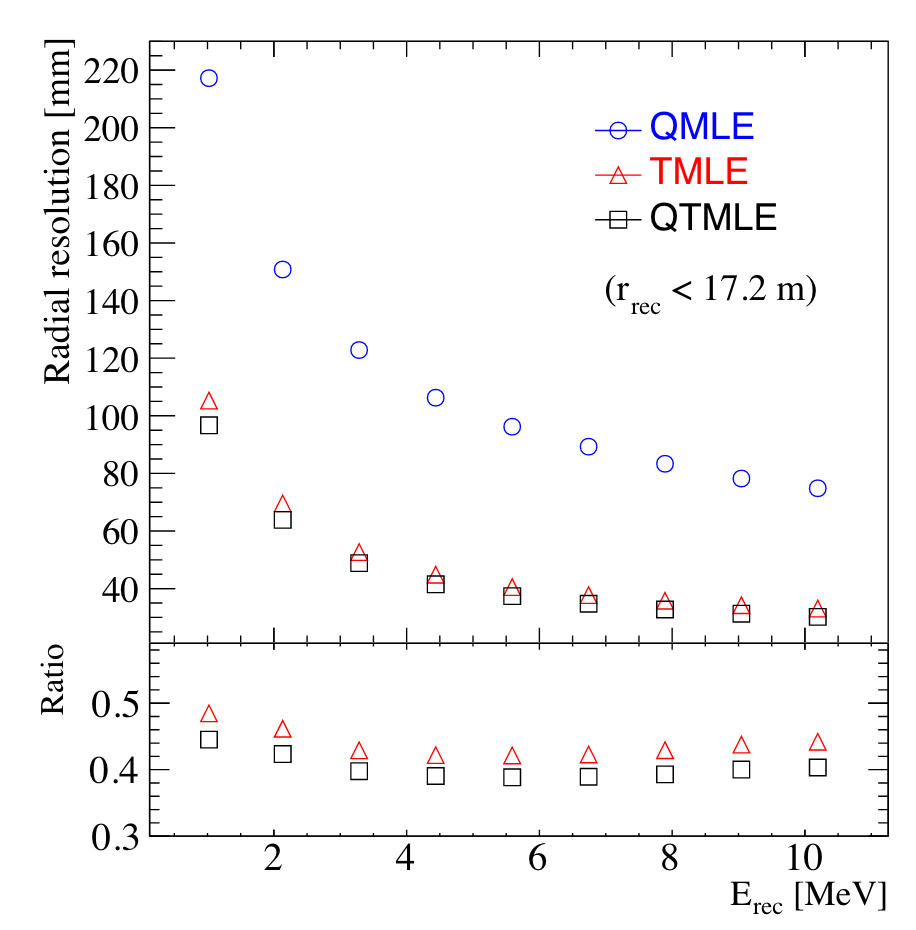
\includegraphics[width=\textwidth]{images/juno/reco/radial_qtmle.png}
    \caption{Radial resolutions of the likelihood-based algorithm TMLE, QMLE and QTMLE}
  \end{subfigure}
  \hfill
  \begin{subfigure}{0.48\linewidth}
    \centering
    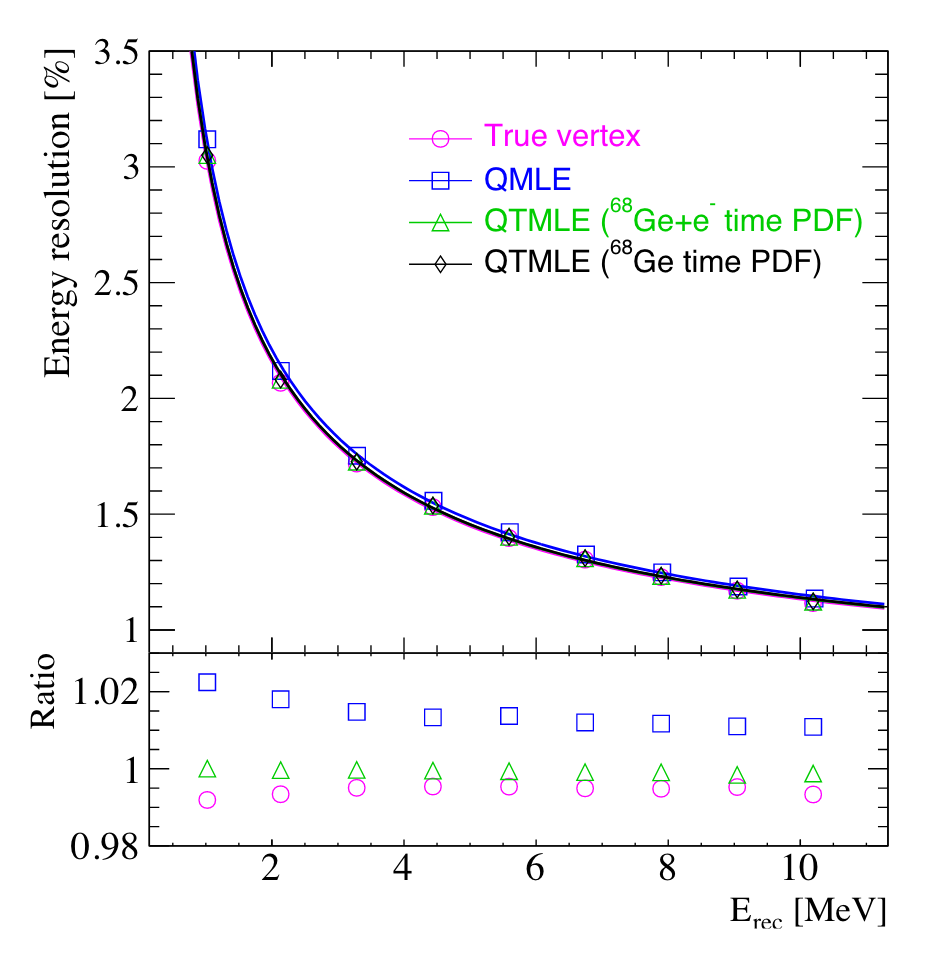
\includegraphics[width=\textwidth]{images/juno/reco/energy_qtmle.png}
    \caption{Energy resolution of QMLE and QTMLE using different vertex resolutions}
  \end{subfigure}
  \caption{}
  \label{fig:juno:rec:qtmle}
\end{figure}

Data driven methods prove to be performant in the energy and vertex reconstruction given that we have enough calibrations sources to produce the PDF. In the next section, we'll see another type of data-driven method based on machine learning.

\subsection{Machine learning for reconstruction}
\label{sec:juno:ml}

Machine learning (ML) is family of data-driven algorithms that are inferring behavior and results from a training dataset. A overview of methods and detailed explanation of the Neural Network (NN) subfamily can be found in Chapter \ref{sec:ml}.

The power of ML is the ability to model complex response to a specific problem. In JUNO the reconstruction problematic can be expressed as follow: knowing that each PMT, large or small, detected a given number of PE $Q$ at a given time $t$ and their position is $x,y,z$ where did the energy was deposited and how much energy was it, modeling a function that naively goes:
\begin{equation}
    \mathbb{R}^{5 \times N_{pmt}} \longmapsto \mathbb{R}^4
\end{equation}
It is worth pointing that while this is already a lot in informations, this is not the rawest representation of the experiment. We could indeed replace the charge and time by the waveform in the time window of the event but that would lead to an input representation size that would exceed our computational limits. Also, due to those computational limits, most of the ML algorithm reduce this input phase space either by structurally encoding the information (pictures, graph), by aggregating it (mean, variance, ...) or by exploiting invariance and equivariance of the experiment (rotational invariance due to the sphericity, ...).

For machine learning to converge to performant algorithm, a large dataset exploring all the phase space of interest is needed. For the following studies, data from the monte carlo simulation presented in Section \ref{sec:juno:software} are used for training. When the detector will be finished calibrations sources will be complementarily be used.

\subsubsection{Boosted Decision Tree (BDT)}

On of the most classic ML method used in physics in last years is the Boosted Decision Tree (see Chapter \ref{sec:ml:bdt}). They have been explored for vertex reconstruction \cite{qian_vertex_2021} et for energy reconstruction \cite{qian_vertex_2021, gavrikov_energy_2022}.

For vertex and energy reconstruction a BDT was developed using the aggregated informations presented in \ref{tab:juno:rec:bdt_vertex}.

\begin{table}[ht]
  \centering
  \begin{tabular}{l|r}
    Parameter & description \\
    \hline
    $nHits$ & Total number of hits \\
    $x_{cc}, y_{cc}, z_{cc}, R_{cc}$ & Coordinates of the center of charge \\
    $ht_{mean}, ht_{std}$ & Hit time mean and standard deviation
  \end{tabular}
  \caption{Features used by the BDT for vertex reconstruction}
  \label{tab:juno:rec:bdt_vertex}
\end{table}
Its reconstruction performances are presented in Figure \ref{fig:juno:rec:ml_res}.

A second and more advanced BDT, subsequently named BDTE, that only reconstruct energy use a different set of features \cite{gavrikov_energy_2022}. They are presented in the table \ref{tab:juno:rec:bdte}

\begin{table}
  \centering
  \begin{tabular}{|c|c|}
    \hline
    AccumCharge &  $ht_{5\%-2\%}$ \\
    $R_{cht}$ & $pe_{mean}$ \\
    $z_{cc}$ & $J_{cht}$ \\
    $pe_{std}$ & $\phi_{cc}$ \\
    nPMTs &  $ht_{35\%-30\%}$\\
    $ht_{kurtosis}$ & $ht_{20\%-15\%}$ \\
    $ht_{25\%-20\%}$ & $pe_{35\%}$ \\
    $R_{cc}$ & $ht_{30\%-25\%}$ \\
    \hline

  \end{tabular}
  \caption{Features used by the BDTE algorithm. $pe$ and $ht$ reference the charge and hit-time distribution respectively and the percentages are the quantiles of those distributions. $cht$ and $cc$ reference the barycenters of hit time and charge respectively}
  \label{tab:juno:rec:bdte}
\end{table}

\subsubsection{Neural Network (NN)}
The physics have shown a rising for Neural Network (NN) in the past years for event reconstruction, notably in the neutrino community \cite{abbasi_graph_2022, reck_graph_2021, collaboration_convolutional_2021, dune_collaboration_neutrino_2020}. Three type of neural networks have explored for event reconstruction in JUNO Deep Neural Network (DNN), Convolutional Neural Network (CNN) and Graph Network (GNN). More explanation about those neural network can be found in Chapter \ref{sec:ml}.

The CNN are using 2D projection of the detector representing it as an image with two channel, one for the charge $Q$ and one for the time $t$. The position of the PMTs is structurally encoded in the pixel containing the information of this PMT. In \cite{qian_vertex_2021}, the pixel is chosen based on a transformation of $\theta$ and $\phi$ coordinates to the 2D plane and rounded to the nearest pixel. A sufficiently large image has been chosen to prevent two PMT to be located in the same pixel. An example of this projection can be found in Figure \ref{fig:juno:rec:cnn_proj}. The performances of the CNN can be found in Figure \ref{fig:juno:rec:ml_res}.

\begin{figure}[ht]
  \centering
  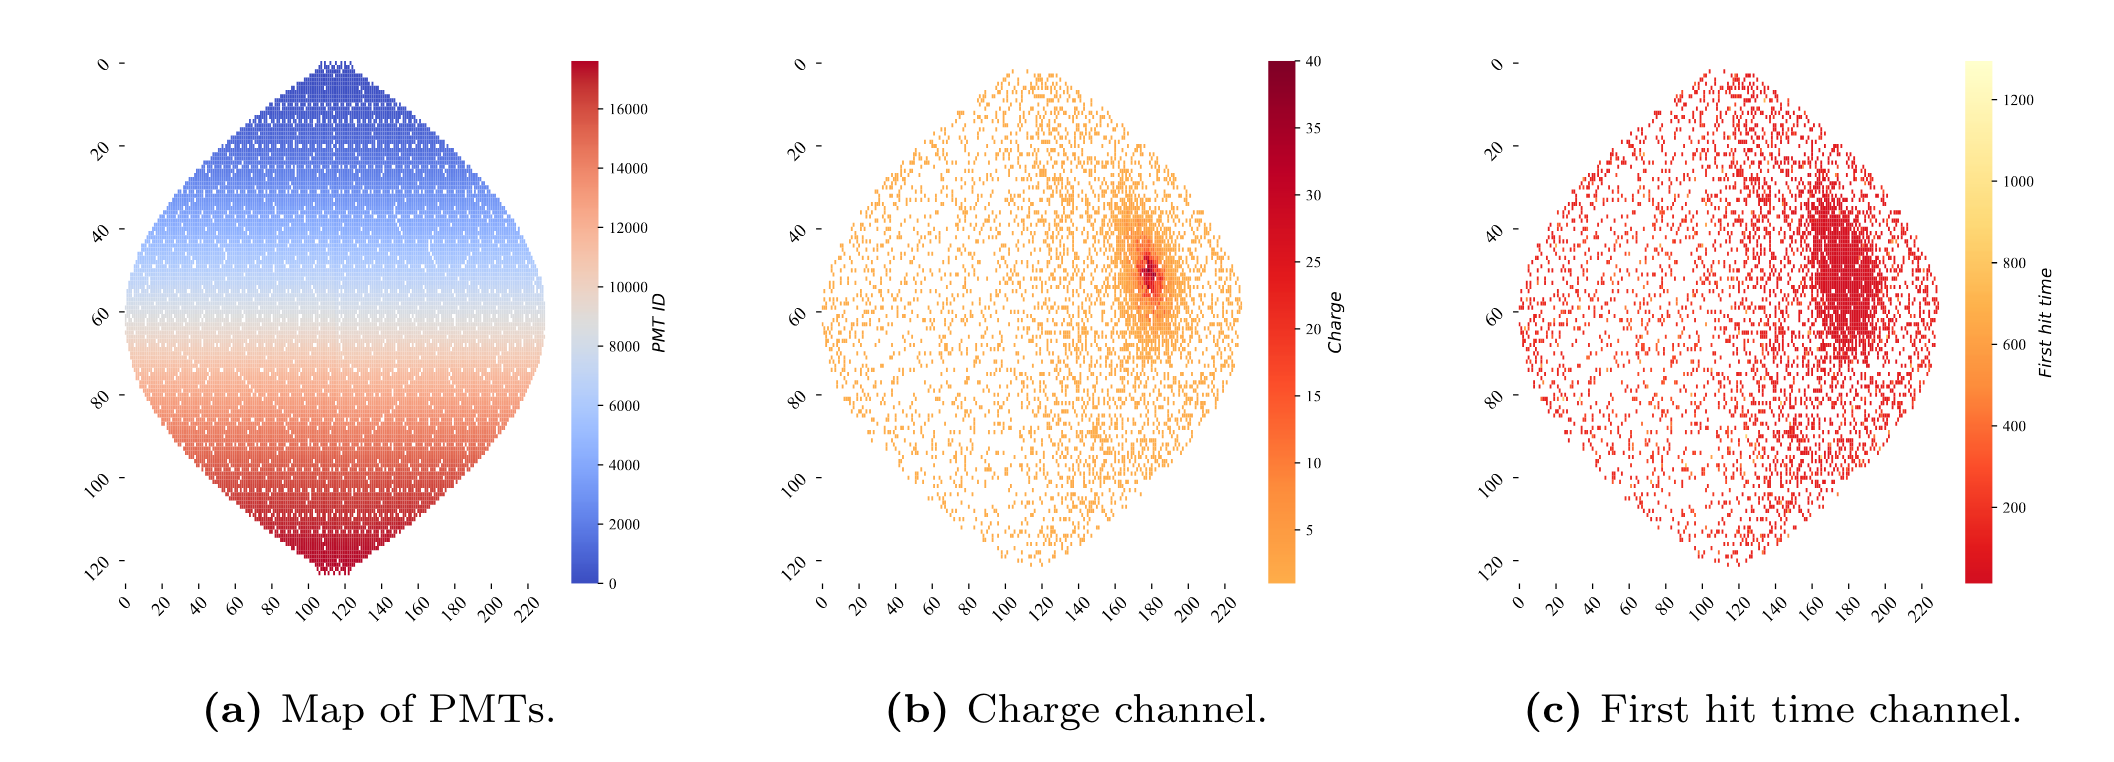
\includegraphics[width=\linewidth]{images/juno/reco/cnn_proj.png}
  \caption{Projection of the LPMTs in JUNO on a 2D plane. (a) Show the distribution of all PMTs and (b) and (c) are example of what the charge and time channel looks like respectively}
  \label{fig:juno:rec:cnn_proj}
\end{figure}

Using 2D have the upside of encoding a large part of the informations structurally but loose the rotational invariance of the detector. It also give undefined information to the neural network (what is a pixel without PMT ? What should be its charge and time ?), cause deformation in the representation of the detector (sides of projection) and loose topological informations.

One of the way to present structurally the sphericity of JUNO to a NN is to use a graph: A collection of objects $V$ called nodes and relations $E$ called edges, each relation associated to a couple ${v_1, v_2}$ forming the graph $G(E, V)$. Nodes and edges can hold informations or features. In \cite{qian_vertex_2021} the nodes, are geometrical region of the detector as defined by the HealPix \cite{gorski_healpix_2005-1}. The features of the nodes are aggregated informations from the PMTs it contains. The edges contains geographic informations of the nodes relative positions.

This data representation has the advantages to keep the topology of the detector intact. It also permit the use of rotational invariant algorithms for the NN, thus taking advantage of the symmetries of the detector.

The neural network then process the graph using Chebyshev Convolutions \cite{defferrard_convolutional_2017}. The performances of the GNN are presented in Figure \ref{fig:juno:rec:ml_res}.


\begin{figure}[ht]
  \centering
  \begin{subfigure}{0.48\linewidth}
    \centering
    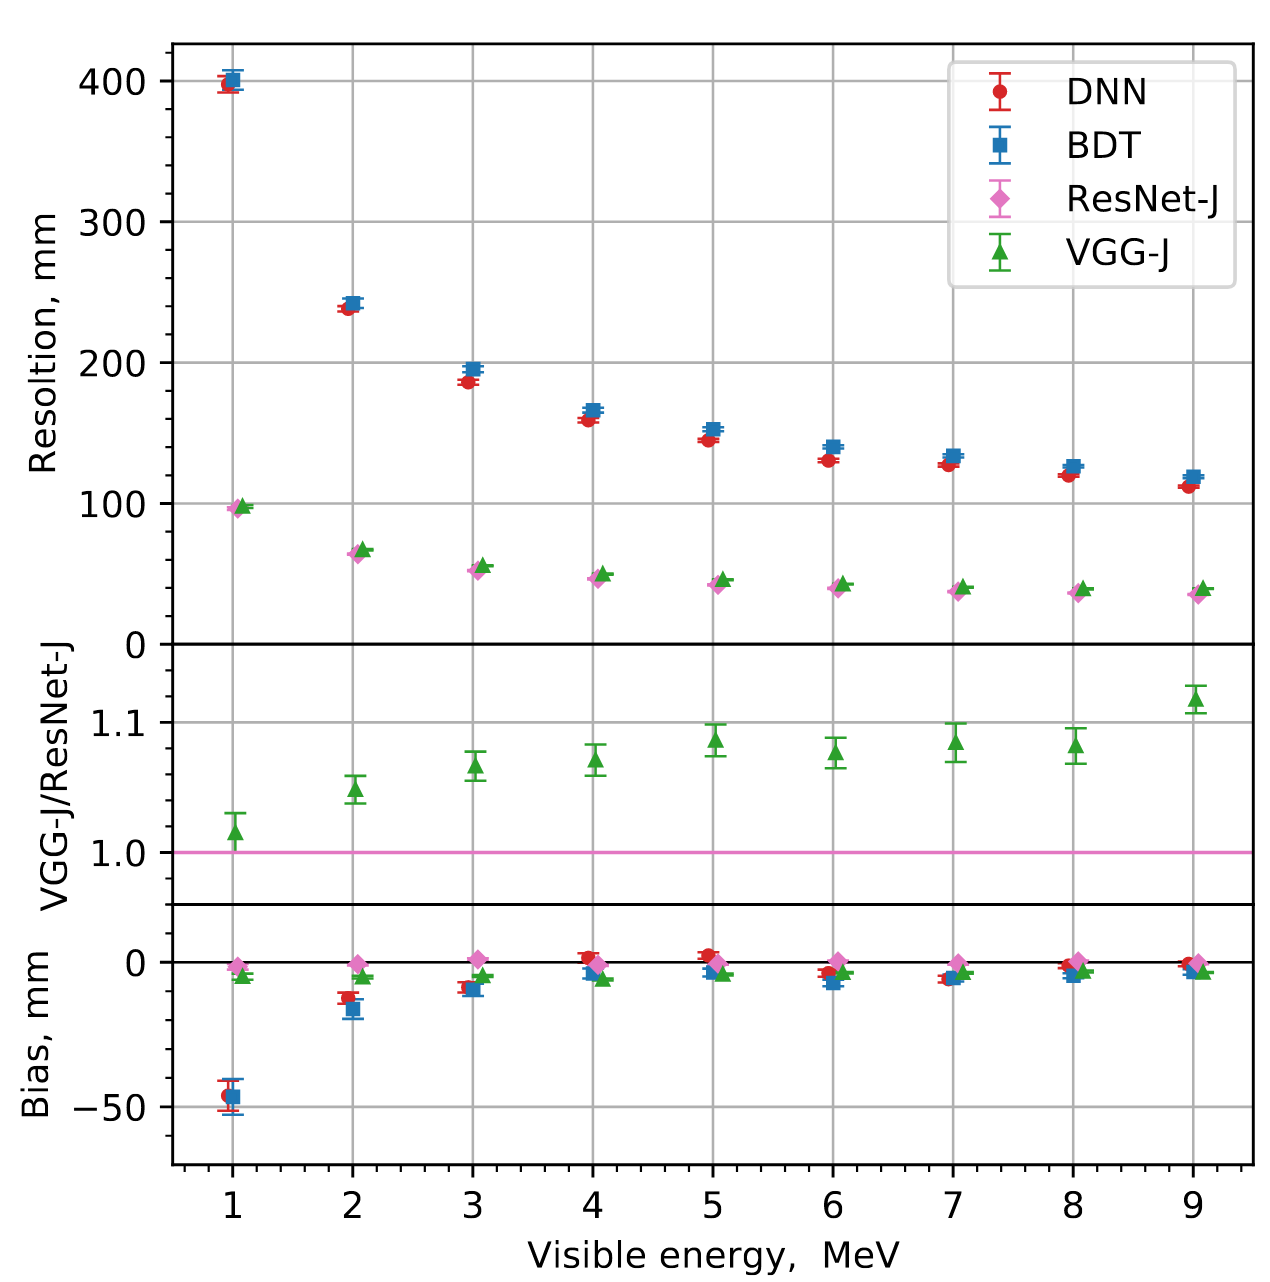
\includegraphics[width=\linewidth]{images/juno/reco/ml_vertex.png}
  \end{subfigure}
  \hfill
  \begin{subfigure}{0.48\linewidth}
    \centering
    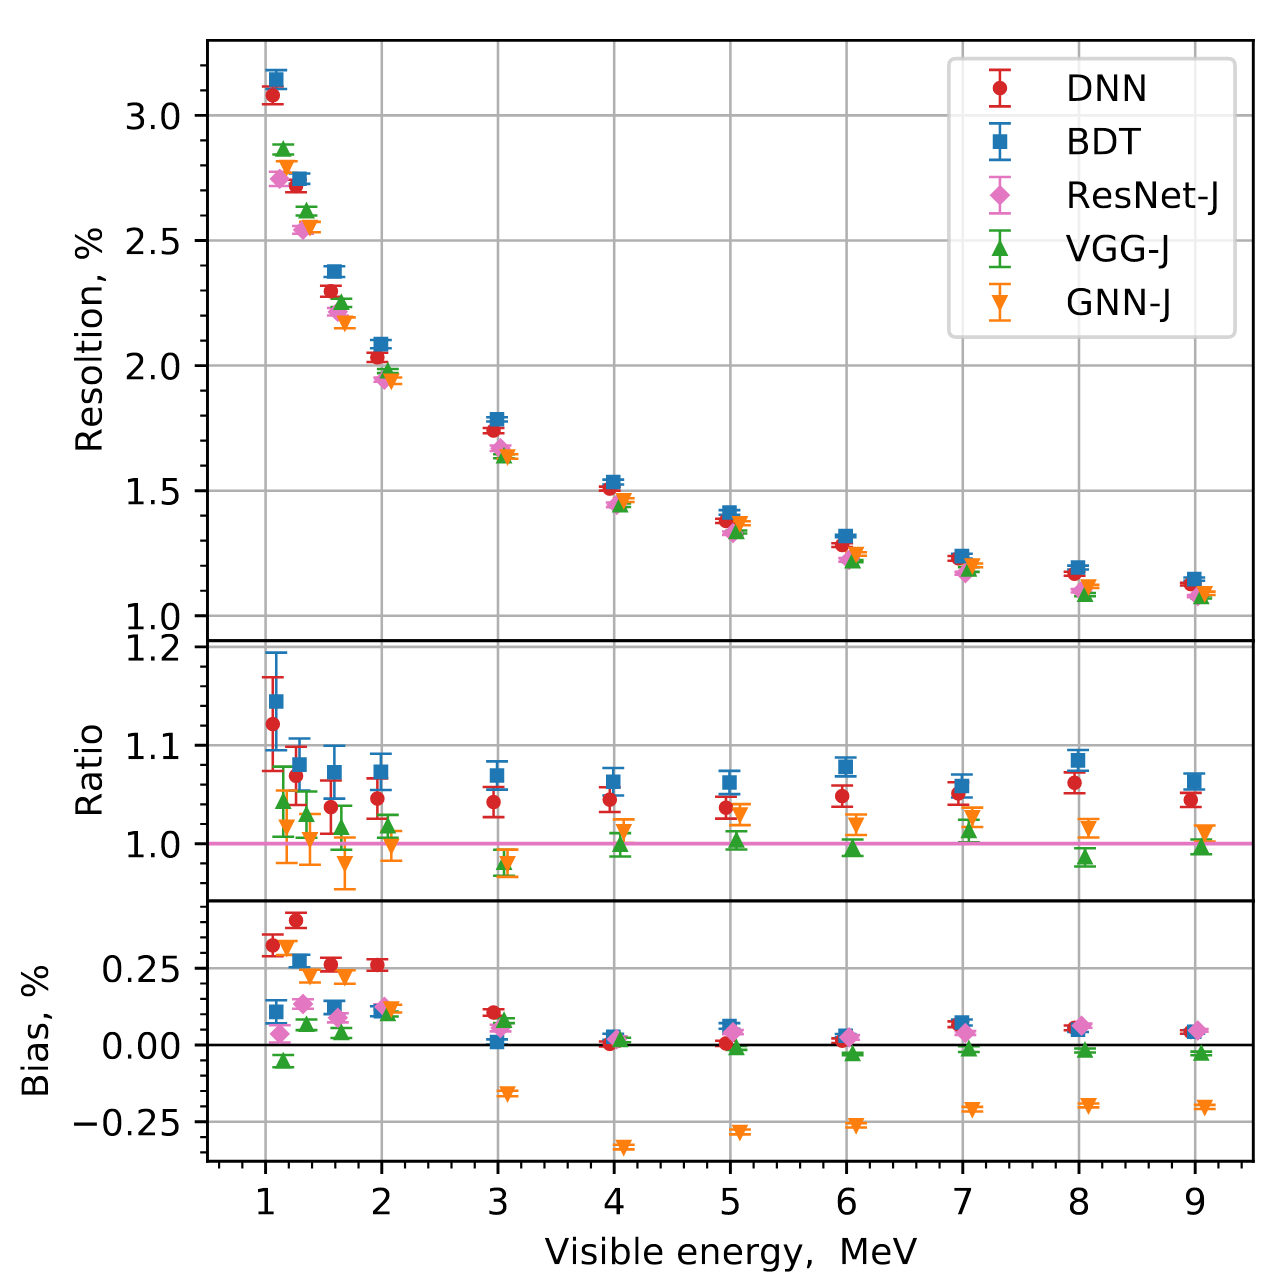
\includegraphics[width=\linewidth]{images/juno/reco/ml_energy.png}
  \end{subfigure}
  \caption{Radial (left) and energy (right) resolutions of different ML algorithms. The results presented here are from \cite{qian_vertex_2021}. DNN is a deep neural network, BDT is a BDT, ResNet-J and VGG-J are CNN and GNN-J is a GNN.}
  \label{fig:juno:rec:ml_res}
\end{figure}

Overall ML algorithms show similar performances as classical algorithms in term of energy reconstructions with the more complex structure CNN and GNN showing better performances than BDT and DNN. For vertex reconstruction, the BDT and DNN show poor performance while CNN are on the level of the classical algorithms.

\subsection{Physics results}

The oscillation parameters are directly extracted from the minimization procedure and the error can be estimated directly from the procedure. For the NMO, the data are fitted under the two assumption of NO and IO. The difference in $\chi^2$ give us the preferred ordering and the significance of our test. Latest studies show that the precision on oscillation parameters after six year of data taking will be of 0.2\%, 0.3\%, 0.5\% and 12.1\% for $\Delta m^2_{31}$, $\Delta m^2_{21}$, $\sin^2\theta_{12}$ and $\sin^2\theta_{13}$ respectively \cite{juno_collaboration_sub-percent_2022}. The expected sensitivity to mass ordering is $3\sigma$ after 6.5 years \cite{juno_collaboration_juno_2022}.

\section{Summary}

JUNO is one the biggest new generation neutrino experiment. Its goal, the measurements of oscillation parameters with unprecedented precision and an NMO preference at the 3 sigma confidence level, needs an in depth knowledge and understanding of the detector and the physics at hand. The characterisation and calibration of the detector are of the utmost importance and the understanding of the detector response in its resolution and bias is capital to be able to correctly carry the high precision physics analysis of the neutrino oscillation.

In this thesis, I explore the usage of data-driven reconstruction methods to validate and optimize the reconstruction of IBD events in JUNO in the chapters \ref{sec:jcnn}, \ref{sec:jgnn} and \ref{sec:janne} and the usage of the dual calorimetry in the detection of possible mis-modelisation in the theoretical spectrum \ref{sec:joint_fit}.
\end{document}
